\documentclass[11pt,a4paper,openright,oneside,oldfontcommands,UKenglish]{memoir}
%%% preamble %%%
%\usepackage[natbibapa]{apacite} % for citations
%\usepackage{cite}
%\usepackage{biblatex}
%\usepackage[dvips]{graphicx}  % this does not work with PDF images
%\usepackage{times}   % this changes the font
%\usepackage[dvips]{color} % original
\setsecnumdepth{subsection} % this numbers also the subsections 
\usepackage[square]{natbib} %[comma,sort&compress]
\usepackage{graphicx}
\usepackage{rotating}
\usepackage{amsmath}
\usepackage{amsfonts}
\usepackage{type1cm}
\usepackage{lettrine}
\usepackage{mathrsfs}
\usepackage{color,soul}
\usepackage{multirow}
\usepackage{pdflscape}
\usepackage{upgreek}
\usepackage{longtable}
%\usepackage{subcaption}
\newsubfloat{figure}
\usepackage{amssymb}
%\usepackage{bbm}
\usepackage{csquotes}
\usepackage{etoolbox}
\usepackage{nomencl}
\usepackage{makecell}
\usepackage{graphbox}
\usepackage[final]{pdfpages}
\usepackage{apalike}

%%% set margins %%%
%\setlrmarginsandblock{40mm}{20mm}{*}  % left right margins
%\setulmarginsandblock{35mm}{40mm}{*}  % upper lower margins

\setlrmarginsandblock{35mm}{30mm}{*}  % left right margins
\setulmarginsandblock{30mm}{30mm}{*}  % upper lower margins
\setheadfoot{\headheight}{15mm}
\checkandfixthelayout  % this puts the layout into effect

%----
\usepackage{todonotes}
%\reversemarginpar
%----

%%% customise chapter style %%%
\makeatletter 
\makechapterstyle{thesis}{%
	\renewcommand{\chapnamefont}{\normalfont\LARGE\sffamily}
	\renewcommand{\printchaptername}{\raggedleft\chapnamefont \@chapapp}
	\renewcommand{\chapnumfont}{\normalfont\LARGE\sffamily}
	\renewcommand{\chaptitlefont}{\normalfont\HUGE\sffamily}
	\renewcommand{\printchaptertitle}[1]{%
		\hrule \vskip\onelineskip \raggedleft \chaptitlefont ##1}
	\renewcommand{\afterchaptertitle}{\vskip\onelineskip \hrule\vskip \afterchapskip}}
\makeatother

%%% set line spacing %%%
\DisemulatePackage{setspace}
\usepackage{setspace}
%\onehalfspacing
\doublespacing

%%% define custom commands %%%
\newcommand{\specialcell}[2][c]{%
  \begin{tabular}[#1]{@{}l@{}}#2\end{tabular}}

\newcommand{\boldalpha}{\mbox{\boldmath$\alpha$}}
\newcommand{\boldsigma}{\mbox{\boldmath$\sigma$}}
\newcommand{\boldxi}{\mbox{\boldmath$\xi$}}

\newcommand{\q}[1]{``#1''}
\newcommand{\red}[1]{\textcolor{red}{#1}}
\newcommand{\blue}[1]{\textcolor{blue}{#1}}
\DeclareMathOperator*{\argmin}{argmin}
\DeclareMathOperator*{\argmax}{argmax}

\chapterstyle{thesis}

\setsecheadstyle{\Large\sffamily\raggedright} 
\setsubsecheadstyle{\large\sffamily\raggedright} 
\setsubsubsecheadstyle{\normalsize\sffamily\raggedright}

\raggedbottomsectiontrue

\usepackage[rm,small]{caption}
\setlength {\captionmargin}{20 pt}

%%% define graphics paths %%%
\graphicspath{{./2gp/}{./3nkernels/}{./4covariant_kernels/}{./5model_selection/}{./6m_ffs/}{./7gp_wf/}}


% La commande qui tue (mais qu'on peut probablement perfectionner):
% 3 paramètres: - préfixe des images - suffixe (extension) des images - options d'affichage des images
\makeatletter
\newcommand\image[3]{
  \@tempcnta\number161
  \advance\@tempcnta-\value{page}
  \divide\@tempcnta2
  \IfFileExists{#1\number\@tempcnta .#2}
  {\includegraphics[#3]{#1\number\@tempcnta .#2}}{}}
\makeatother
% Pb: il faut lui dire combien de page le document a...
% (parce que je sais pas encore faire automatiquement)

% Où l'on place les animations dans les coins.

\setlength{\headwidth}{\textwidth} 
%\addtolength{\headwidth}{\marginparsep} 
\addtolength{\headwidth}{1cm}

\copypagestyle{thesis}{ruled}

\makerunningwidth{thesis}{\headwidth}

\makeheadrule{thesis}{\headwidth}{\normalrulethickness}
\makefootrule{thesis}{\headwidth}{\normalrulethickness}{\footruleskip}

\makeheadposition{thesis}{flushright}{flushleft}{flushright}{flushleft}

%\makeevenfoot{thesis}{}{\thepage}{}

\makeoddfoot{thesis}{}{}{
  \setlength\unitlength{1cm}
  \begin{picture}(0,0)
    \put(-3.5,-1.5){
      \image{./flip/gr}{eps}{scale=0.09}
    }
  \end{picture}
}

\makeatletter
\makepsmarks{thesis}{% 
\let\@mkboth\markboth 
\def\chaptermark##1{\markboth{##1}{##1}}% % left & right marks 
\def\sectionmark##1{\markright{% % right mark 
\ifnum \c@secnumdepth>\z@ 
\thesection. % section number 
\fi 
##1}} 
}
\makeatother

\makeevenhead{thesis}% 
{\normalfont\sffamily\thepage}{}{\normalfont\sffamily\leftmark} 
\makeoddhead{thesis}% 
{\normalfont\sffamily\rightmark}{}{\normalfont\sffamily\thepage} 

\makeevenfoot{thesis}{}{}{}


%%% define hyperreferences links %%%
\usepackage[hyphens]{url}
%\usepackage[naturalnames, breaklinks]{hyperref}
%\hypersetup{colorlinks=true,breaklinks=true}
%\hypersetup{		% customise hyperreff
%	colorlinks   = true, 
%	urlcolor     = blue, 
%	linkcolor    = blue, 
%	citecolor   = blue }

\soulregister\cite7
\soulregister\ref7

\hyphenation{se-que-ste-ring}
\hyphenation{mo-le-cules}
\hyphenation{haemo-lytic}
\hyphenation{back-map-ped}

\makenomenclature
%%% to only compile a specific chapter %%%
%\includeonly{1introduction/introduction} 
%\includeonly{2gp/gp} 
%\includeonly{3nkernels/nkernels}
%\includeonly{4covariant_kernels/covariant_kernels}
%\includeonly{5model_selection/model_selection} 
%\includeonly{6m_ffs/m_ffs}
%\includeonly{7gp_wf/gp_wf}
%\includeonly{8conclusions/conclusions}
% --------------------------------------%
\begin{document}

\pagestyle{plain}

%\frontmatter % roman numbers
\mainmatter  % arab numbers 

% Title Page 
%\thispagestyle{empty}

%\begin{center}
%\Large {\textsc{Multiscale Hybrid Simulation\\ of Brittle Fracture}}
%\end{center}

%\cleardoublepage

\thispagestyle{empty}

\begin{center}


{\textsc {\Huge Elucidating self-assembly}}\\
%
\vspace{.15in}
%
{\textsc {\Huge and antimicrobial strategies}}\\
%
\vspace{.15in}
%
{\textsc {\Huge of synthetic peptides:}}\\
%
\vspace{.15in}
%
{\textsc {\Huge an in silico investigation}}
%
\vspace{1.5in}

{\Large Irene Marzuoli}

\vspace{.4in}

{\textsc {\large Randall Centre of Cell and molecular Biophysics}}

\vspace{0.15in}

{\textsc {\large King's College London}}

%\vspace{1.7in} original
\vspace{1in}
%\includegraphics[height=3cm]{pem.eps}
%\hspace{1.5cm}

\includegraphics[height=3cm]{KCL_logo.pdf}

\vspace{1in}

{\textsc {\large This dissertation is submitted for \\ 
the degree of Doctor of Philosophy}}

\vspace{0.5in}

{\textsc {\large September 2019}}

\end{center}

\cleardoublepage

%\onehalfspacing

\makeatletter
\renewcommand{\@pnumwidth}{2em}
\renewcommand{\@tocrmarg}{3em}
\setlength{\cftbeforechapterskip}{.9em}
\makeatother

%%%%%%%%%%%%%%%%%%%%%%%%%%%%%%%%%%%%%%%%%%%%%%%%%%

\thispagestyle{empty}

\begin{vplace}[0.15]

\begin{center}
%\large
\it{To my parents, for letting me go}
\end{center} 

\end{vplace}


%%%%%%%%%%%%%%%%%%%%%%%%%%%%%%%%%%%%%%%%%%%%%%%%%%

\cleardoublepage
%%% empty page
\newpage
\thispagestyle{plain} % empty
\mbox{}
%%

%%%%%%%%%%%%%%%%%%%%%%%%%%%%%%%%%%%%%%%%%%%%%%%%%%

\thispagestyle{empty}
\chapter*{Declaration}

%\section*{Declaration of Originality} 

\noindent This dissertation describes work I have carried out between October 2016 and September 2019 at the Randall Centre of King's College London, under the supervision of Professor Franca Fraternali (first supervisor) and Dr. Chris D. Lorenz (second supervisor).

\vspace{.2cm}

\noindent This dissertation contains material appearing in the following articles:

\begin{itemize}
%\end{itemize}}[(i)]
\item ...
\end{itemize}

\noindent In addition to the above, I have contributed to the following publications during the course of my PhD:

\begin{itemize}
%
\item ...
%
\end{itemize}
%


%\section*{Statement of Length}

\vspace{.2cm}

\noindent This dissertation is my own work and contains nothing which is the outcome of work done in collaboration with others, except as specified in the text and acknowledgements.
%
It has not been submitted in whole or in part for any degree or diploma at this or any other university.

\vspace{1.5cm}

\begin{raggedleft}
Irene Marzuoli \\
September 2019

\end{raggedleft}


%%%%%%%%%%%%%%%%%%%%%%%%%%%%%%%%%%%%%%%%%%%%%%%%%%%
%
%\cleardoublepage
%%%% empty page
%\newpage
%\thispagestyle{plain} % empty
%\mbox{}
%%%
%
%%%%%%%%%%%%%%%%%%%%%%%%%%%%%%%%%%%%%%%%%%%%%%%%%%%

\thispagestyle{empty}
\chapter*{Acknowledgements}
%
...


%%%%%%%%%%%%%%%%%%%%%%%%%%%%%%%%%%%%%%%%%%%%%%%%%%%
%
%\cleardoublepage
%%%% empty page
%\newpage
%\thispagestyle{plain} % empty
%\mbox{}
%%%
%
%%%%%%%%%%%%%%%%%%%%%%%%%%%%%%%%%%%%%%%%%%%%%%%%%%%

\thispagestyle{empty}
\chapter*{Summary}

\begin{center}

{\Large\sffamily Elucidating self-assembly and antimicrobial strategies of synthetic peptides an in silico investigation}

\vspace{.2cm}

{\large\sffamily Irene Marzuoli}

\vspace{.03cm}

{\large\sffamily King's College London}
%
\vspace{.2cm}

\end{center}
%
\noindent
%
...
%
...
%%%%%%%%%%%%%%%%%%%%%%%%%%%%%%%%%%%%%%%%%%%%%%%%%%

\cleardoublepage
%%% empty page
\newpage
\thispagestyle{plain} % empty
\mbox{}
%%

%%%%%%%%%%%%%%%%%%%%%%%%%%%%%%%%%%%%%%%%%%%%%%%%%%
 
\tableofcontents*

\cleardoublepage

\listoffigures*

%%% List of symbols and acronyms %%%

% name
\renewcommand{\nomname}{List of symbols and acronyms}

% spacing 
\newlength{\nomitemorigsep}
\setlength{\nomitemorigsep}{\nomitemsep}
\setlength{\nomitemsep}{-\parsep}

% groups
\renewcommand{\nomgroup}[1]{
%
\itemsep\nomitemorigsep
\ifthenelse{\equal{#1}{A}}{\item[\textbf{Acronyms}]}{
%
\ifthenelse{\equal{#1}{B}}{\item[\textbf{ccc}]}{
%
\ifthenelse{\equal{#1}{K}}{\item[\textbf{vvv}]}{
}}}
\itemsep\nomitemsep}


\printnomenclature[7.6em]

\cleardoublepage
%%% empty page
\newpage
\thispagestyle{plain} % empty
\mbox{}
%%


\thispagestyle{empty}







\pagestyle{thesis}

\copypagestyle{chapter}{thesis}
\makeevenhead{chapter}{}{}{} 
\makeoddhead{chapter}{}{}{} 

\makeheadrule{chapter}{\headwidth}{0cm}
%\makefootrule{chapter}{\headwidth}{0cm}{0cm}

\makeoddfoot{chapter}{}{}{
  \setlength\unitlength{1cm}
  \begin{picture}(0,0)
    \put(-3.5,-1.5){
      \image{./flip/gr}{eps}{scale=0.09}
    }
  \end{picture}
}

%\setlength{\parindent}{0pt} % set indentation length for new paragraph
%\setlength{\parskip}{10pt}  % set skip length for new paragraph

%\begin{KeepFromToc}
%	\tableofcontents
%\end{KeepFromToc}

%\newpage

%\listoffigures


%%%%%%%%% Acronyms %%%%%%%%%

 \nomenclature[A]{AM}{Antimicrobial}
 \nomenclature[A]{AMP}{Antimicrobial Peptide} 
 \nomenclature[A]{CAMP}{Cationic Antimicrobial Peptide} 
 \nomenclature[A]{AMR}{Antimicrobial Resistance} 
 \nomenclature[A]{MDR}{Multi-drug Resistance} 
 \nomenclature[A]{AAV}{Adeno-associated virus}
 \nomenclature[A]{VLP}{Virus-like particle}
 \nomenclature[A]{CRISPR}{Clustered Regularly Interspaced Short Palindromic Repeats}
 \nomenclature[A]{OM}{Outer Membrane}
 
 \nomenclature[A]{TEM}{Transmission Electron Microscopy}
 \nomenclature[A]{AFM}{Atomic Force Microscopy}
 \nomenclature[A]{SEM}{Cryo-scanning Electron Microscopy}
 
 \nomenclature[A]{ML}{Machine Learning}
 \nomenclature[A]{MD}{Molecular Dynamics}
 \nomenclature[B]{MC}{Monte Carlo}
  
\nomenclature[K]{BBB?FDA?PEG?LPS?}{ll}

%%%%%%%%% Math conventions %%%%%%%%%

%\nomenclature[B0]{$a \mid \mathbf{a} \mid \mathbf{A} \mid \mathbb{A}$}{Scalar, vector, matrix and block matrix}
%
%\nomenclature[B1]{$\mathbf{a}^{\rm{T}} \mid \hat{\mathbf{a}} $}{The transpose $\mathbf{a}$ and the unit vector in the direction of $\mathbf{a}$}
%
%\nomenclature[B3]{$\sim$}{Distributed according to or approximately equal to}
%
%\nomenclature[B31]{$\mathcal{GP}$}{Gaussian stochastic process}
%
%\nomenclature[B32]{$\langle \cdot \rangle $}{Expectation with respect to a Gaussian stochastic process}
%
%\nomenclature[B40]{$\boldsymbol{\theta}$}{Vector of hyperparameters}
%
%\nomenclature[B41]{$\ell \mid \sigma_n^2$}{Lengthscale and noise hyperparameter}
%
%\nomenclature[B42]{$\mathcal{D}$}{Dataset}
%
%\nomenclature[B43]{$N$}{Number of training points}
%
%\nomenclature[B5]{$\mathcal{O}(\cdot)$}{Computational complexity}



\chapter{Introduction} \label{chapter:intro}

\lettrine{``P}{hilosophical introduction"} to be finished/modified when the work is finished...

%\lettrine{T}{heory} stays to experiment as experiment stays to nature. And science stays to technology as technology stays to life.

%To navigate this huge gap is the scientist call, in an effort to bring the extremes closer, giving a model of how nature functions, or to enrich the space in between, inventing new realities. Technology bridges every day this very gap: every consequence of our abstract thinking is technology, an hidden layer of inductions and deductions which brings us from abstract principle to solutions. Computers, the ultimate technology, are emulating increasingly better and more efficiently this process, sparing us the awareness of the complex mechanisms which thread the problem to its solution. It was in the past two centuries that we witnessed such an evolution of techniques, inventions and machineries that we can now exploit years of theoretical thinking by using tools in practical problems to eventually modify nature in every daily activities. If in the past nature was the mystery and the human intervention on it was simple to understand, now on the contrary many basic principles of the physics laws are clear to most of us but human inventions became increasingly complex, condensing centuries of discoveries in simple, efficient tools. We use planes, drugs and the internet not because we perfectly understand how they work, but because we trust the collective knowledge we, as humans, have accumulated so far.

%Out of the many fields at service of the humanity wellness, the most challenging and still far away from being exhausted is the understanding and manipulation of the human body and mind. While machines - in the broadest sense possible - can perform actions in our place, they can't yet think and live on their own. It is striking how we are finally scratching the understanding of these two entities, mind and body, in the same historical moment, at a point where computers imitates the human reasoning \cite{AlphaGo, AIreview} and biological materials are turned into semi functional organs \cite{Rossi2018}. However, we are far from completing the jigsaw of knowledge on these topic. On the contrary with the progression of the techniques available to investigate various fields, we realise how vast is the space to be explored. It is then a logical consequence that the modern scientist is becoming more and more specialised, drifting away from the comprehensive knowledge owned by scientists up to two centuries ago; but exactly because the full picture is challenging, every project aimed at understanding an aspect of these enormously vast themes, no matter how tiny the subject is, is involved in a network of efforts, in the hope and trust that piecewise knowledge can build a unique and organic corpus.

%This thesis places itself in the domain of understanding how the human body works - how the (non) equilibrium of life is possible and how human intervention can be possible. The tiny and narrow topic it covers wants to explore one possible way in which we help the body to heal itself and to defend itself against external malicious agents. To correct those processes that go wrong means life, and we are biologically and emotionally pushed towards actions that prolong and improve life and have always looked at ways of curing ourselves. But the body evolved in the past blind to reason, on the contrary taking advantage of multiple defences and barrier which secured it from the failure of the reasoning, and it is know to us often a mystery, as we struggle to understand many of its components, letting aside the whole picture.

%Quite blindly then we developed in the past a medicinal science which managed to be of service to the human envelope, in what was a remarkable game of trial and error resorting to magic first and to our intelligence last \cite{history_medicine_review}. The risk and inevitable failures tracing the path were a necessary toll to the utmost necessity of keeping healthy, safe and - ultimately - alive. In a history resembling the evolution of technology, we resorted to nature for beneficial molecules \cite{above}, which we called drugs in the initial fuzziness existing between healing and deadly, but then humans started identifying the beneficial principle in these natural remedies \cite{other_review_early_drugs?}, and ultimately to produce new molecules \cite{other_review_early_drugs?}. The increasing understanding of how we worked pointed out the many challenges a drug has to withstand to be efficient. And this knowledge poses question: if so many barriers prevent a drug from entering the body, how can infectious agents have found a way to our cells? And if we want to fight those ones instead, why the body cannot recognise these helpful molecules as beneficial ones and is fighting them instead? Are they perhaps damaging for us as well, in some way we have not yet understood?

%Luckily, if knowledge has brought awareness of the complexity of the machine our body is, it started bringing also solutions. We do now have drugs \cite{drug_database}, we know how to selectively deliver some of them \cite{review_drug_delivery}. We have disinfectants \cite{WIDES_database}, and we have antibiotics to fight pathogens \cite{ABXdatabaseJhopkins}. We do know what we are composed of \cite{Mitchess1945}, and how this material rearranges in organelle, cells, organs. And we know some of the mechanisms concerting these parts together \cite{what?}.

%We are finally moving in the direction of the magic bullet envisioned a century ago by Nobel Prize Paul Ehrlich, who dreamed of a 'personalised and tailored drug' able to target specific molecular defects while being harmless - if not beneficial - to the other cells \cite{Strebhardt2008}. Such success would condense in a tiny amount of space a century of efforts in understanding the human body. But we still miss many pieces of information as the more we zoom in, the less each single researcher can monitor at once and the more we realize is there to be discovered.

%In this prospect, looking at how one particular molecule behaves with respect to a particular environment, as this thesis does, using a simplified theory (sometimes the only possible) is certainly a tiny fragment of knowledge added to the world of science. But, joint to the other scientific output from the community, it is a necessary, meaningful and promising fragment.

\vspace{1cm}
(...thus) This introduction is meant to give an overview of the many different challenges the fields of medicine and bioengineering have faced in recent years. These challenges have promoted the research on self-assembling antimicrobial peptides, despite they were not a primary source of interest in these fields, as other materials and concepts were deemed more suitable to solve the tasks coming along the way. It is therefore important to clarify the landscape of such other solutions and approaches to understand and value why a change in the research focus has come to age. Figure \ref{fig:intro} provides a work flow of this introductory chapter to help the reader in identifying the sections of interest.

\begin{figure}
\begin{center}
\Large{\textbf{Motivations of the work: a graphical abstract}}\par\bigskip
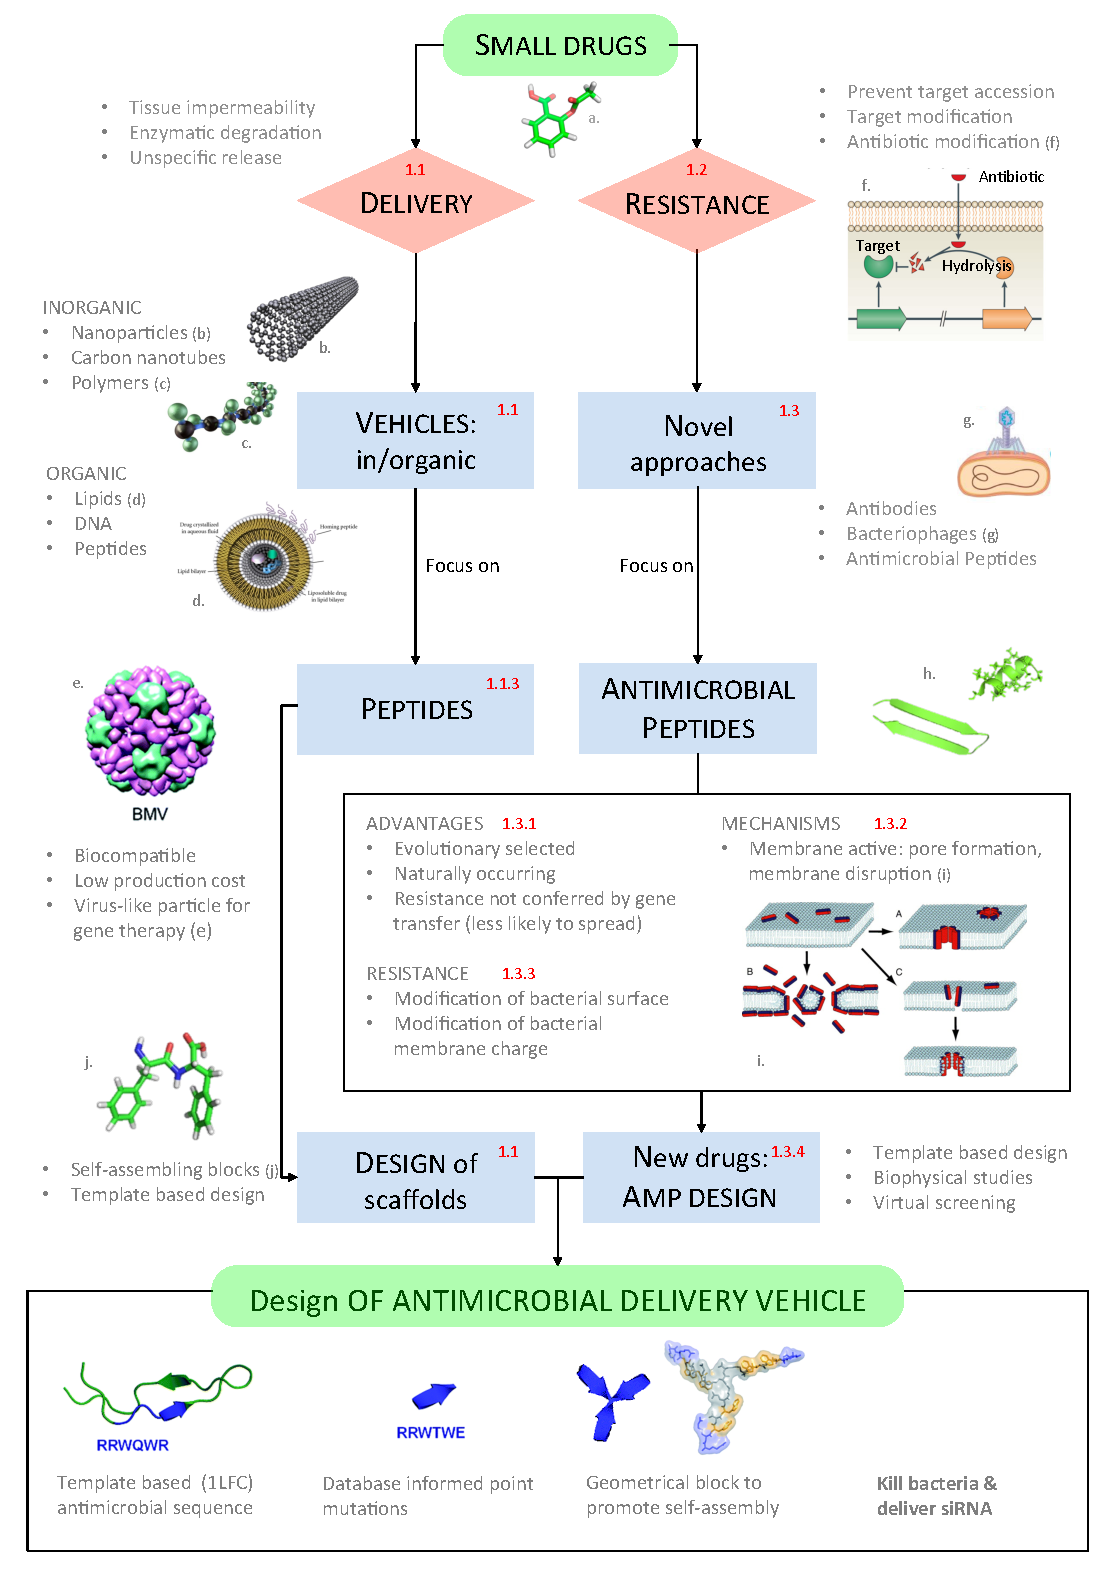
\includegraphics[width = \textwidth]{1introduction/pics/scheme_intro}
\caption[Graphical abstract of introduction]{Figures a. (acetylsalicylic acid) and j. (diphenyl-alanine) in bond representation. Remaining figures adapted from: b. [--]; c. \cite{poly}; d. \cite{lipo}; e. \cite{Schoonen2014}, f. \cite{Blair2014}; g. \cite{phage}; h. \cite{Torres2019}; i. \cite{Nguyen2011}; k. \cite{Castelletto2016}} \label{fig:intro}
\end{center}
\end{figure}

\clearpage

\section{Antimicrobial resistance}

For most of the last century, the development of new drugs rotated around the paradigm that a drug is a small inorganic compound (of mass up to 900 Da), which intervenes on a specific target of a mammal or bacterial cell. Very often the targets of interest are (intracellular) proteins: out of the 695 small drugs approved by FDA (the American Food and Drug Administration agency) to target human molecules, 667 acts on proteins. Similarly, 189 of the 198 approved to treat pathogens have a protein as their target \cite{Santos2017}
%
(with all the caveats coming from the challenges of identifying an unambiguous target, especially when the drug binds to a protein complex or to a number of closely related gene products \cite{Santos2017}).

In presenting the aforementioned figures, the data were naturally split among the drugs which act on human molecules, ``repairing" some faulty process in the human body, or the ones active against bacteria, which ``disrupt" the bacterium life cycle in order to kill or prevent the reproduction of the pathogen, commonly named as antibiotics.
%
It appears evident that the pool of drugs available to the second purpose are in substantially lower number than the ones addressing human molecules. This comes from the nature of the action they perform: molecules targeting human proteins need to be highly specific to avoid interference with other proteins or with healthy cells, and in a sufficient number to address the variety of diseases affecting the human body.
%
Antibiotic must be non-toxic for human cells as well, i.e.\ their target must not be shared between mammal and bacterial cells, but there is a less stringent requirement on their selectivity against different bacterial species. On the contrary, it is often useful to have a broad-spectrum compound. This cross-species efficacy and at the same time non-toxic property is obtained thanks to the evolutionary relationship among bacterial species, and between bacteria and humans: while the first are closely related, and therefore share homologous proteins with very similar structures, humans have less architectures in common with them, allowing for a resilience against bacteria-targeting drugs.
%
To be precise, the set of bacterial species is very diverse and the cross-species effectiveness of some drugs does not extend to the whole bacterial population. This is actually demonstrated to be a positive feature, given the large amount of beneficial bacteria that live in symbiosis with the human body (especially in the gut) and that must be preserved for an optimal wellness.

In the framework described above, it is understandable that first-time research on antibiotics was satisfied with the development of a handful of potent, broad-spectrum compounds.
%
Penicillin, the first of them to be synthetically produced, was isolated from a mould in 1928 by Alexander Fleming. It acts inhibiting the formation of peptidoglycan cross-links in the bacterial cell wall, binding to the enzyme responsible for its catalysis, and thus preventing the wall complete formation \cite{Gordon2000} (for further details on bacterial cell membrane structure see Section \ref{sec:host-defense-peptides}).
%
As foreseen from Fleming himself in his Nobel Prize acceptance speech, some species of bacteria quickly became immune to penicillin, and this was achieved in many ways: either by production of penicillase, an enzyme that degrades penicillin, or by subtle changes in the structure of the penicillin-binding proteins to prevent penicillin binding, or again by removal of the drug outside of the cell through specially re-purposed efflux pumps \cite{???}.

The mechanisms just outlined are not an exceptional characteristic of penicillin, and many drugs lost their effectiveness against some bacteria since their discovery till nowadays, urging the research of new ones on a constant basis. By now, a broad knowledge has been gathered on how bacteria escape the action of a drug: this understanding helps interpreting the pitfalls of existing drugs and identifying the characteristics sought in the developments of new compounds.


\subsection{Mechanisms of antimicrobial resistance to small drugs} \label{sec:AMR_mechs}
Antimicrobial resistance can manifest through many different mechanisms, which can be grouped in three main classes, in line with the three processes mentioned in the example of the penicillin resistant bacteria.

\begin{figure}[h]
\begin{center}
\subbottom[]{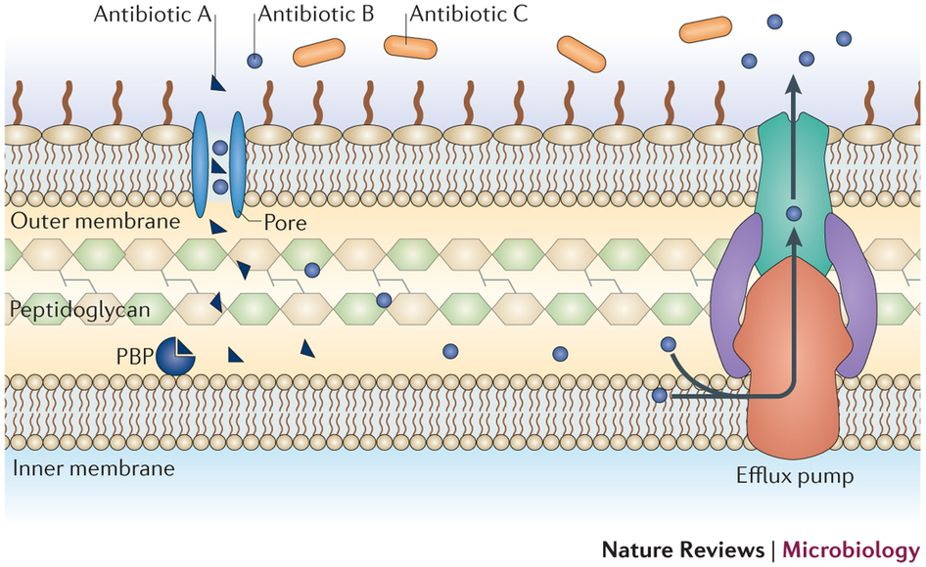
\includegraphics[width=0.6\linewidth]{1introduction/pics/amr1} \label{fig:amr1}} \\
\subbottom[]{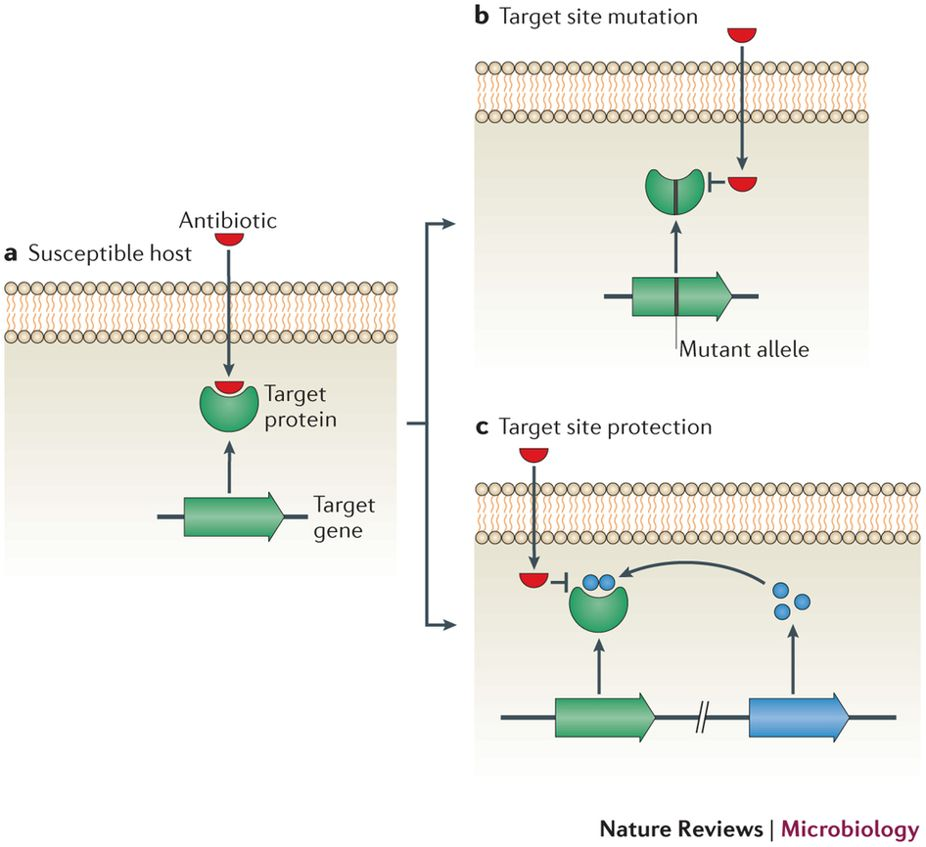
\includegraphics[height = 0.36\textheight]{1introduction/pics/amr3} \label{fig:amr2}}
\hspace{0.5cm}
\subbottom[]{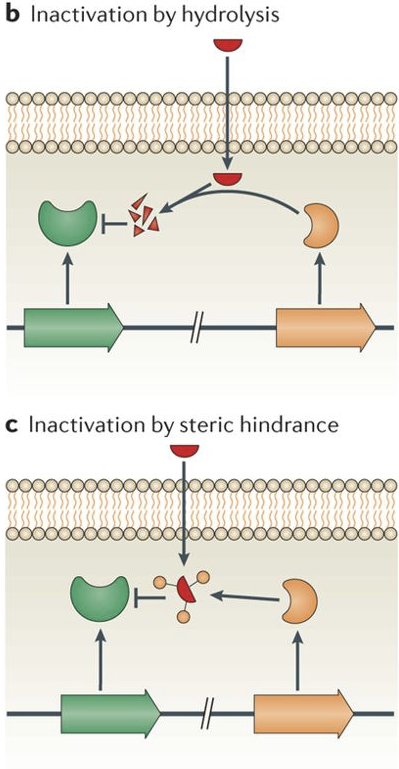
\includegraphics[height = 0.36\textheight]{1introduction/pics/amr4_half} \label{fig:amr3}}
\caption[Mechanisms of antimicrobial resistance to small drugs]{Mechanisms of antimicrobial resistance to small drugs. (a) Intrinsic mechanisms of resistance (removal of antibiotic B by efflux pump and inaccessibility of antibiotic C to the PBP target because of membrane impermeability). (b) Target site change via mutation or protection. (c) Direct interactions with antibiotics causing its disruption or structural modification. Reproduced from \cite{Blair2014}.} \label{fig:amr}
\end{center}
\end{figure}

\paragraph{Prevention of access to target}
A first class of resistance mechanisms aim at minimising the intracellular concentration of the antibiotic preventing its penetration or maximising its efflux in the eventuality it has entered the cell (Figure \ref{fig:amr1}).
%
Not all the molecules can enter the cell permeating the membrane, and this holds particularly for hydrophilic antibiotics tackling Gram-negative bacteria which are intrinsically less permeable that Gram-positive ones because of the additional presence of the outer membrane \cite{Delcour2009} (for further details on the bacterial membrane structure, see Section \ref{sec:host-defense-peptides}).
%
These molecules must then be imported into the cell through outer-membrane porin proteins \cite{Vargiu2012,Kojima2013}. Resistance arise when porins are either replaced with more selective channels, which prevent the antibiotic penetration, or down regulated so the internal concentration of the drug does not reach a critical concentration \cite{Lavigne2013}. Porin-coding genes can also accumulate multiple mutations, to acquire the selectivity they lack in their wild type \cite{Poulou2013}.

A complementary strategy to prevent drug influx is to employ bacterial efflux pumps. Some of them are denominated multidrug resistance (MDR) efflux pumps for their effectiveness in the task and are produced by many bacteria \cite{Floyd2010,Ogawa2012}, but, additionally, can be transferred via plasmids to other bacterial species \cite{Dolejska2013}. Indeed, bacteria are able to exchange genetic material with other individuals via small rings of DNA in a process called conjugation \cite{????}, so that the advantageous resistant genotypes can spread quickly across species.
%
Over-expression of such efflux pump is observed in multidrug-resistant bacteria, triggered by exposition to the drug, and proceeding via mutation in the relative regulatory network, \cite{Abouzeed2008}, or simply as a response to environmental signals \cite{Nikaido2011}.


\paragraph{Change or modification of the antibiotic target}
The second class of resistance mechanisms works modifying the antibiotic target: most antibiotics bind to their substrate with high affinity and specificity, thus small modifications in the target structure can disrupt an efficient binding, still allowing the target to maintain its normal function (Figure \ref{fig:amr2}).

Mutations of some residues in the binding pocket (upon mutation in the gene coding for it) or post-translational protection of the target via addition of chemical groups are equally wide spread mechanisms.
%
Notable examples of the first include the development of methicillin and linezolid-resistant strains of S. aureus \cite{Shore2011,Billal2011}. Again, it is interesting to notice that several of these mutations are acquired by horizontal gene transfer from other bacterial species, so that resistance development in one specie promotes quickly the insurgence of resistance in other ones.
%
For the second, the most relevant mechanism of chemical group addition is methylation, which for example is very common when the drug target are rRNA subunits \cite{Long2006}).


\paragraph{Direct modification of antibiotics}
Finally, bacteria can destroy drugs, usually by hydrolysis, or modify them by transfer of a chemical group (Figure \ref{fig:amr3}).

The first example historically discovered of drug-degrading enzyme is penicillinase (a $\beta$-lactamase) which destroys penicillin \cite{Abraham1988}. Since then, thousands of similar enzymes have been identified that can modify antibiotics of different classes \cite{Livermore2008,Nordmann2011}:
%
these enzymes co-evolves with newly developed drugs, to include in their spectrum of action new compounds of composition similar to the ones they were originally effective on \cite{Woodford2013}.

Antibiotics constituted by large molecules with many exposed hydroxyl and amide groups are instead particularly susceptible to modification by addition of chemical groups. Many enzymes are responsible for this, and according to the chemical moiety added they are grouped in acetyltransferases, phosphotransferases and nucleotidyltransferases \cite{Wright2005}.

\hspace{0.5cm}
\\
All together, the recent progress in understanding the mechanisms of antimicrobial resistance has helped in directing the development of new drugs, in particular the modification and the improvement of existing compounds to escape the resistance developed by bacteria. To ultimately employ the existing drugs at best, it is important to understand also the dynamics of AMR, beyond its molecular mechanisms, to device the most effective strategies of drug administration.


\subsection{Course of antimicrobial resistance} \label{sec:course_AMR}
In the first stages of the insurgence of antimicrobial resistance (AMR) against a given drug, some strains of bacteria are not damaged by the standard doses of the drug as they came to possess some natural occurring mutations in their genome which promote an escape mechanism invalidating the drug effectiveness \cite{Kapoor2017,Blair2014}. Usually, only a small population of bacteria is resistant  in the first moments, however the resistant population will replicate faster that the peers of the same species because it is more fit in an environment challenged by the presence of the drug. It is noteworthy that this fitness might not be optimal in a natural drug-free environment - and indeed the wild population has not been selected for that genotype - but under the pressure derived from the treatment, other characteristics result more advantageous.
%
In the short time scale it is usually sufficient to increase the doses of the drug to re-gain efficiency against the target, but resistant species can usually adapt to higher doses of the same \cite{????}. Moreover, high drug doses are not always applicable due to the severe side effects they are connected to.

As already mentioned, the spread of resistance between bacterial cells and even between species is very effective as bacteria exchange genetic material through conjugation.
%
Therefore, despite AMR is an evolutionary mechanism, the fast pace at which bacteria replicates, their enormous population (in terms of individuals), and the relative easy horizontal gene transfer through conjugation, place the insurgence of resistance well within the human lifespan time scale \cite{????}.

It is then clear that this complex problem depends on many variables: the casual appearance of resistant individuals, the transfer of information between them, the relative gain in fitness that the mutation implies, but also the dosage and time line of the drug administration. Many mathematical models have been implemented to understand the issue \cite{Birkegard2018,Niewiadomska2019}, but it is known that some particular strategies of drug administration are worse than other, favouring the proliferation of so called ``super" bugs.
%
One example of bad administration strategy is the underdosage of antibiotics: a low drug load is likely to harm but not kill pathogens, and rather promote the fitness of resistant ones. In a sort of ``gym" or ``vaccination" process for bacteria, an underdosed drug would kill the weakest individuals but strengthen the resistant population, which would now be fitted for the challenges of higher doses \cite{????}.
%
Similarly, the abuse of antibiotics puts an high pressure on the pathogenic populations, which is desirable but at the same time can induce a faster emergence of escape mechanisms \cite{????}.

In this context it must be noticed that many drugs are bacteriostatic agent as opposed to bactericidal: i.e.\ they prevent the bacterium growth rather than kill it, as they are meant to control the bacteria reproduction and slow down the damage while host defence mechanisms eradicate them.
%
Thus if an high dosage of a bactericidal agent may extinguish the bacterial population and eradicate the disease, for bacteriostatic drugs, once they are removed, bacteria start again the reproduction cycle.

It is then clear that the antibiotic landscape is a dynamic entity in which newly discovered drugs enter, while others exit after having been exploited for years, and must be monitored carefully and kept populated. The severity of the AMR issue is such that it has been raised to the status of national emergency in several countries, including UK. Indeed, abuse or misuse of antibiotic can take many forms and strict regulations on the health, agricultural and food industry sector must be taken to prevent its loss of efficacy, as we are leaving the century in which antibiotics were discovered, to enter a phase in which we count the number of the ones loosing efficacy \cite{Oneill2016}.


\section{Alternative antibiotic strategies: antimicrobial peptides}
In the landscape sketched above, it is evident that the development of novel drugs is of crucial importance. Even more beneficial would be to have at disposal a new paradigm for their design, in order to attack pathogens in a completely novel way, avoiding to target pathways which are known to lead easily to the development of antimicrobial resistance. Several novel materials have been developed for the task, not to rely on small molecules and exploit different mechanisms of action, for example antibodies, bacteriophages or antimicrobial peptides \cite{Mantravadi2019}.

While the use of pathogen-specific antibodies relies on the mechanisms of the host immune system, bacteriophages therapy employs viruses which infect bacteria and archea rather than eukarya.
%
But are antimicrobial peptides the focus of this thesis: indeed peptides can have an active role against bacteria when their sequence possesses specific characteristics. Such active sequences, capable of damaging and/or killing pathogens, are referred to as antimicrobial peptides. The following subsections will explore their characteristics, modes of action and the response of bacteria against them. It is crucial to understand the knowledge available versus the questions that are still open in order to direct the efforts of future research. This holds in particular when the investigation proceeds by the use of simplified models, as meaningful results can proceed only if such modelling is performed in a sensible and informed fashion.

\begin{figure}
\begin{center}
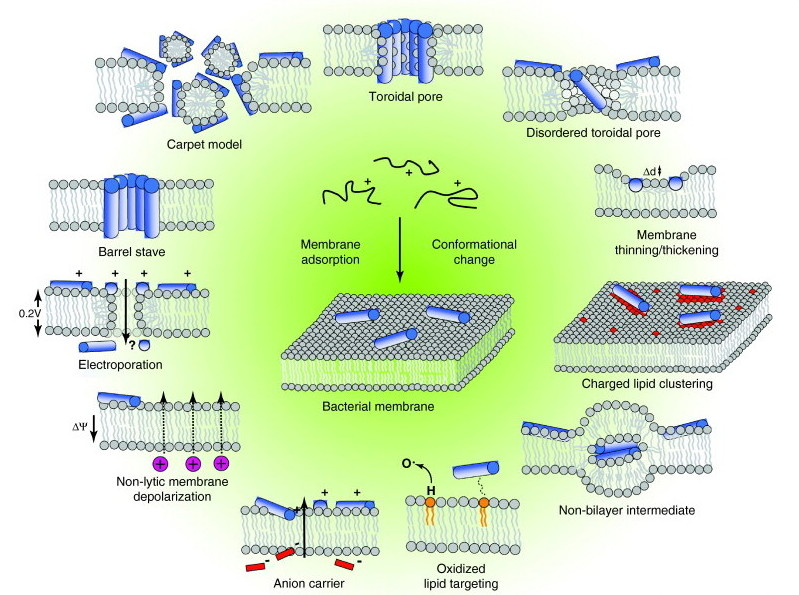
\includegraphics[width = 0.7\textwidth]{1introduction/pics/amp_mech.jpg}
\caption[Antimicrobial peptides]{Events occurring at the bacterial cytoplasmic membrane following initial antimicrobial peptide (AMP) adsorption. Reproduced from \cite{Nguyen2011}.} \label{fig:amp}
\end{center}
\end{figure}


\subsection{Membrane active peptides} \label{sec:host-defense-peptides}
Antimicrobial peptides (AMPs) are naturally produced by eukarya, either as stand-alone sequences or embedded in larger proteins, as a first, weak, and broad-spectrum defence against bacteria \cite{Nguyen2011}.
%
This pool of molecules has been selected though evolution to be active against pathogens, suggesting that they are weakly prone to provoke resistance reactions in the microbes they attack.

To exploit their potential and engineer AMP-like molecules, a careful characterisation and classification of such peptides must be done. This task has been carried on throughout the past decades but it is complex, so that up to date there are many peptides with ascertained antimicrobial activity for which the mode of action is still not fully understood \cite{Ebbensgaard2015}. However, some general characteristics of these sequences and some of the mechanisms they employ have emerged.
%
Unsurprisingly, AMPs are heterogeneous in shape, targets and mode of action, to tackle the different challenges bacteria pose. Their size can vary between 6 and 59 amino acids \cite{Brogden2005}: despite being small with respect to the average size of a protein in the human body, these macromolecules are hundreds of times larger than small molecule drugs and as such they penetrate and act on bacteria differently with respect to small compounds.

The most common target of AMPs is the bacterial membrane. Many of them cause disruption of the physical integrity of the microbial membrane while others translocate into the cytoplasm to act on intracellular targets, and the combination of the two is not uncommon either \cite{Hancock2006} (Figure \ref{fig:amp}). In general, it is widely accepted that membrane interaction is a key factor for the direct antimicrobial activity of AMPs \cite{Nguyen2011}.

As such, we propose a brief overview of the structure of this membrane \cite{Silhavy2010}, and of its differences with the one of mammalian cells.


\paragraph{Structure of bacterial membrane}
The determinant driving the interaction between AMPs and bacterial membranes is the positive charge that many AMPs present, opposed to the negative charge of the latter.
%
It is striking that such simple mechanism, based on the presence of a certain number of negatively charged lipids, holds across many bacterial species despite the great variability found in their membrane composition.
%
Indeed, based on the differences in their cell envelope structure, bacteria are classified into two macro families, Gram-positive and Gram-negative.
%
In Gram-positive bacteria, the cytoplasmic membrane is surrounded by a thick peptidoglycan layer, while for Gram-negative bacteria this membrane (which assumes the name of internal one) is surrounded by a thin peptidoglycan layer as well as an outer membrane \cite{Lin2016}.

Starting from the inside and proceeding outwards, the cytoplasmic membranes of both Gram-positive and Gram-negative bacteria are rich in phospholipids like phosphatidylethanolamine, which is neutral, and phosphatidylglycerol, cardiolipin, and phosphatidylserine, which have negatively charged headgroups, highly attractive for positively charged AMPs. This is often sufficient to promote the preferential interaction between this membrane and peptides - provided they reach it.
%
Perturbation of this membrane is highly disruptive as many functions are associated to it: as bacteria do not possess organelles, all the membrane related proteins reside and perform their function on the inner membrane. 

In the case of Gram-negative bacteria, the inner membrane, together with the outer one, delimits the periplasm space, an aqueous cellular compartment, which allow to sequester harmful substances and to transport nutrients.
%
Proceeding outward, inside the periplasm is situated the peptidoglycan cell wall. Repeated units of this substance, made of a disaccharide cross-linked by penta-peptide side chains (from which the name), constitute the rigid skeleton of Gram-negative bacterial cells. Damage in the peptidoglycan layer results usually in living but not viable cells, therefore it is fundamental for cell life.
%
Grafted to the skeleton through Braun’s lipoproteins is the outer membrane. This membrane presents an asymmetric structure: phospholipids are present in the inner leaflet, while the outer one is composed of glycolipids, mainly lipopolysaccharides (LPS). This complex molecules consist of lipid A, which presents multiple fatty acids, and a polysaccharide, made of an inner core, covalently bond to the lipid, an outer core attached to the inner and finally a repetitive glycan polymer (O-antigen). The O-antigen is the molecule exposed by Gram-negative bacteria to the external environment and thus is the target of antibodies recognition. 

Given the complexity of the Gram-negative cell envelope, and especially the presence of the LPS layer, these bacteria are particularly impermeable to hydrophilic molecule, which are usually imported within the cell through porins and similar transmembrane proteins.

For Gram-positive bacteria, the inner membrane is enveloped in a thick peptidoglycan layer. If its thickness in Gram-negative bacteria is reaches few nanometers, in Gram-positive ones it spans from 30 to 100 nm. Its composition is similar to the one described above, with some variations present among different bacteria, for example in the nature of the peptidic linker or in its precise position. This thick layer is threaded by long anionic polymers (the teichoic acids), mainly composed by glycerol phosphate, glucosyl phosphate, or ribitol phosphate repeats. Disseminated in this layer there are several surface proteins with various functions, among which adhesins, which attach to components of the host extracellular matrix.

Gram-positive are generally more permeable because they do not possess a double-membrane structure, nevertheless the peptidoglycan later they are coated with constitute a challenge for drug delivery.


\paragraph{Comparison with mammalian membrane}
The fact that AMPs tackle negatively charged membranes is crucial for their selectivity, i.e.\ the fact that they are harmless for the mammalian cells they are produced from \cite{Glukhov2005}. Indeed, mammalian cells have a different membrane composition. They present a single membrane, which is very rich in protein (up to 50\% of its volume) and in lipids, with a small percentage of carbohydrates, mainly embedded in glycoproteins, which promote the cell-cell recognition.

The lipidic component is abundant in zwitterionic phospholipids such as phosphatidylethanolamine, phosphatidylcholine, and sphingomyelin, providing a neutral net charge \cite{Spector1985,vanMeer2008}.
%
Strictly speaking, some negatively charged lipids are present in a few mammal cell types, however they are located in the inner leaflet, while the zwitterionic phospholipids are more abundant in the outer leaflet, in an asymmetric composition \cite{???}.
%
This structure promotes weaker interactions between AMPs and mammalian cells with respect to bacterial ones, as the former is driven mainly by hydrophobic interactions, while the latter by electrostatic ones.
%
Furthermore, the mammalian cell membrane has a high content of cholesterol \cite{Yeaman2003, Lai2009}, a sterol fat, which is proposed to stabilise the membrane regulating its fluidity across the differences of physiological temperatures, and it is also though to favour a better accommodation of the perturbations caused by AMPs \cite{Zasloff2002}.

Another relevant difference between bacterial and mammal cells is that the first ones typically have a higher transmembrane potential - the difference of electrostatic potential between the inside and the outside environment: for bacteria it falls between $-130$ and $-150$ mV, while for mammalian cells between $-90$ and $-110$ mV \cite{Yeaman2003,Matsuzaki2009,Ebenhan2014}.
%
Given that a potential generates an electric field across the membrane, the higher it is, the higher the electric field pointing from outside to inside the cell. A field in such direction pushes cationic compounds on the outside of the membrane toward the membrane itself. Therefore the stronger bacterial transmembrane potential may promote an enhanced - and thus disruptive - interaction of AMPs with the cell, contributing to the selectivity of AMPs between bacteria versus mammals \cite{Yeaman2003}.


\subsection{Common mechanisms of action of AMPs} \label{AMP_mechs}
Investigating the perturbation and disruption of a bacterial membrane by antimicrobial peptides is a key point of this work, therefore it is important to highlight the mechanisms known so far through which AMPs reach this outcome.
%
As already mentioned, many AMPs have a positive charge which facilitates the binding to the membrane via charge-charge recognition; accordingly, Arginine and Lysine residues are usually abundant in AMPs sequences. However, the disruptive action takes place through the interaction of the AMP with the hydrophobic core of the membrane, therefore their sequence contains also hydrophobic aromatic residues, especially Tryptophan, which favours the anchoring to the lipid core \cite{Chan2006}.
%
Overall, AMPs resort often to adopt an amphiphatic structure to segregate the hydrophilic from the hydrophobic amino acids and thus act at the interface between membrane and solution. It is interesting to notice that some of them fold into the active structure only nearby the membrane, as they can expose their hydrophobic components to face its core, while in solution these ones are preferentially buried inside to be screened from the solvent \cite{Nguyen2011}.
%
Common folds adopted by AMPs are both $\alpha$-helix or $\beta$-sheet rich structures. Amphiphatic $\alpha$-helices present a charged side which is tailored to face towards the phospholipid head groups and an hydrophobic ones which is favourably buried into the acyl chains core,
%
and a similar arrangement is found for structures rich in $\beta$-sheets include $\beta$-hairpins.


\paragraph{Membrane disruption} Several models have been proposed to describe the exact mechanisms of AMPs penetration after they bind to the cytoplasmatic membrane, and how their combined action leads to membrane permeabilization (Figure \ref{fig:amp}) \cite{Brogden2005,Nguyen2011}.

For example, for a single copy of a amphiphatic helical AMP, the proposed mechanism of action suggests that initially the peptide is attracted with its charged side to the membrane and lies parallel to its plane, with the hydrophobic side unfavourably exposed in solution. Then the helix rearranges to have the two faces in the respective favourable regions. Subsequently, the helix axis starts to form an angle with the membrane plane, and finally inserts deeper into the lipid core, often spanning the full membrane thickness.
%
Similarly, for $\beta$-sheet rich structures, it is suggested that they insert within the membrane after a first flat approach.
%
The final insertion arrangement depends on the peptide characteristics and length, the presence of kinks in its structure (in case of helices), and the interactions with other copies of the peptide.

The picture becomes more complex for oligomer-mediated insertion, i.e.\ when the action is triggered by the combined action of many copies of the peptide.
%
At low peptide to lipid ratio, the favourable configuration is represented by peptides lying parallel to the membrane plane as described previously \cite{Yang2001}, but an increase in peptide concentration triggers the transition to an inserted state where the main axis of the AMP is perpendicular to the membrane. The organisation of AMPs inside the membrane core can assume different configurations, as described below.

The ``barrel-stave" model proposes that AMPs insert perpendicularly into the bilayer. Recruitment of peptides in the same area results in the formation of a transmembrane pore with a central lumen. The walls of the pore are constituted by the hydrophilic face of the peptides, while their hydrophobic side is interacting with the lipid tails around the pore. This model is adopted for example by the $\alpha$-helical AMP alamethicin, which forms voltage-dependent ion channels by aggregation of four to six molecules \cite{Spaar2004}.

In the ``toroidal" pore model instead, the insertion of peptides forces the phospholipid to bend continuously from one leaflet to the other, resulting in a pore defined by both peptides and phospholipids head groups.
%
The toroidal model differs from the barrel-stave model as the peptides are always associated with the lipid head groups even when they are perpendicularly inserted in the lipid  bilayer. Toroidal pores are induced by $\alpha$-helical magainins, protegrins and melittin \cite{Yang2001,Matsuzaki1996,Hallock2003}, and lead to membrane perturbation which extends further away from the pore than in the barrel-stave case, as lipids must rearrange around them.

As a comparison, alamethicin induced barrel-stave pores have an inner and outer diameters of 1.8 nm and 4.0 nm respectively \cite{Spaar2004}, while magainin-induced toroidal pores are larger and can vary in their size, with an inner diameter of 3.0-5.0 nm and an outer diameter of 7.0-8.4 nm, involving about 4 to 7 magainin monomers and about 90 lipid molecules \cite{Matsuzaki1997}.

Finally, in the ``carpet" model, the accumulation of AMPs on the surface of the membrane, laying parallel to it, causes tension in the bilayer and the membrane is then disrupted by peptides in a detergent-like manner, leading to the formation of micelles.
%
The critical threshold concentration triggers a cascade effect, in which formation of the first disruption allows the penetration of AMPs in the inner side of the bilayer. The cooperation between peptides on both sides of the lipid membrane enhances the AMP-induced curvature on the membrane causing accelerated disruption.
%
The ``carpet" model mechanism is observed for peptides presenting an $\alpha$-helical structure (like melittin \cite{Ladokhin2001}) or several helices connected by short loops (ovispirin \cite{Yamaguchi2001}).

The prevalence of examples with an helical structure for the above models derives from the fact that the understanding of how helical AMPs function is often easier than the one of $\beta$-sheet rich structures.
%
Indeed, helices have a well defined fold (at least nearby the membrane environment), a compact structure, and often a clear segregation of complementary patches that can attract other copies of the peptide and thus promote the self-assembly process necessary for the pore formation.

On the contrary, many $\beta$-sheet AMPs have a more flexible structure, and more diversified mechanisms of action \cite{??}.
%
AMPs rich in $\beta$-sheets can be divided into $\beta$-hairpins and peptides from the defensin family \cite{Nguyen2011}.
%
Many representative of the former class disrupt bacterial membranes via formation of toroidal pores: as an example, porcine peptide protegrin I triggers the toroidal pore formation assembling into a $\beta$-barrel structure when in contact with anionic membranes (while it folds into $\beta$-sheet aggregates on the surface of cholesterol containing membranes, thus acting selectivity on bacterial membranes only \cite{Tang2009}).

In the case of defensins, many mechanisms are known according to the specific member of the family \cite{Lehrer2004}.
%
Some form transmembrane pores on planar bilayer when a physiologically relevant negative potential is applied to the membrane \cite{Kagan1990}, while others form oligomers in phospholipid vesicles \cite{Takeuchi2004}.
%
Although various descriptions of membrane damage have been reported, and include ion channels, transmembrane pores and extended rupture of the membrane, they are likely related, being a modulation of a similar acting principle.


\paragraph{Alternative mechanisms of action} Finally, many non-lytic mechanisms are suggested for AMPs, especially for $\beta$-sheet structures: defensin A from P. terramovae reduces the cytoplasmic potassium concentration \cite{Brogden2005}, partially depolarising the inner membrane; tachyplesin from horseshoe crabs is able to bind to the minor groove of DNA, interfering DNA–protein interactions \cite{Yonezawa1992},
%
and bovine lactoferricin can act synergistically with other antimicrobial agents by affecting the transmembrane potential and proton-motive force, resulting in inhibition of ATP-dependent multi-drug efflux pumps \cite{Gifford2005}.
%
Moreover, after translocation within the cell, bovine lactoferricin can also inhibit DNA, RNA and protein synthesis. Section \ref{sec:capzip} will treat in detail the functioning of this AMP, distinguishing its role as membrane active peptide versus intra-cellular targeting compound: indeed, many works have focussed on lactoferricin antimicrobial processes versus locating the section of the sequence performing the membrane disruptive activity \cite{Tomita1994,Schibli1999}, to understand whether it retains the efficacy regardless of the fold.

These and similar strategies of investigations, conducted on several AMPs \cite{???}, provided the discovery of first minimal functioning antimicrobial blocks, which promoted the understanding of how AMPs work in general, boosting the design of synthetic tailored AMPs from specific sequences.


\subsection{Mechanisms of resistance to AMPs}

Antimicrobial peptides are introduced here as a class of new drugs and a possible solution to the crisis of antimicrobial resistance. Any new drug entering the pool of the clinically approved compounds is (at least temporary) a solution to the problem of resistance to known antibiotics, but it must be clarified that bacteria can develop resistance to AMPs too.
%
Never the less, the resistance to their action is generally not based on dedicated genes that are conferred by horizontal gene transfer, as in the case of many antibiotics resistance mechanisms \cite{Peschel2006}. Because of that, a certain increase of resistance after exposure to the drug is to be expected (`MIC creep'), but it is less likely to spread quickly to other species.

Some of the mechanisms of AMPs resistance are similar to the ones employed by bacteria to counteract small molecule drugs, for example over-expression of efflux pumps to dispose of AMPs, degradation of the peptide by extracellular enzymes and sequestration by the bacterial or biofilm matrix to prevent accession to the target \cite{Peschel2006}.

Differently with respect to antibiotics hydrolysis, AMPs proteolitic degradation is operated by proteases, secreted on the extracellular side of the membrane specifically to destroy other proteins. Linear AMP are more prone to this type of degradation \cite{Sieprawska-Lupa2004}, as opposed to the ones presenting disulfide bonds \cite{Peschel2006}, such as defensins, which nevertheless can be hydrolysed by more specific proteases enzymes \cite{Nelson2011}.

Bacteria can also enhance their resistance to AMPs organising into specialised structures known as biofilms. These structures are formed by sessile bacteria adhering to a surface in an organized manner that allows the circulation of nutrients \cite{Costerton1999}.
%
Biofilm bacteria secrete an extracellular matrix with adhesion and protection functions \cite{Jolivet-Gougeon2014}, which effectively repels and/or captures AMPs through exopolysaccharid or capsular polysaccharides.
%
For example polysaccharide intercellular adhesin (PIA) produced by S. aureus and a variety of other bacteria is responsible for the resistance to both cationic AMPs (like HBD-3, LL-37) and the anionic one dermcidin \cite{Vuong2004PIA}: deacetylation of PIA increases its positive net charge, thus repelling more efficiently cationic AMPs, and increasing sequestration of the anionic ones at the same time \cite{Vuong2004}.

It's worth noting that AMPs are nevertheless a promising alternatives in the treatment of biofilm-associated infections: indeed, in this type of infections (where bacteria are growing slowly) it is advantageous to have bactericidal agents such as AMPs, as opposed to bacteriostatic ones which target fast-growing bacteria only, as the majority of traditional antibiotics do \cite{Strempel2014}.

But the most specific mechanism of AMPs resistance concerns modifications of the bacterial cell envelope: bacteria modify the characteristics of their surface to prevent the efficient binding of an AMP, even in the eventuality that the peptide reaches the bacterial envelope intact. 
%
The target of such modifications are different for Gram-positive and Gram-negative bacteria, according to their distinct cell envelopes.
%
Gram-positive bacteria change the structure of their teichoic acids (TA): for example, D-Alanylation of TA observed in S. Aureus adds a positive charge to it, reducing the attraction of cationic AMPs and in turn increasing the cell wall density, so reducing the surface permeability \cite{Saar-Dover2012}.
%
Alternatively they can modify the bacterial peptidoglycan precursor, lipid II, which has a key role in the formation of the cell wall ad is often targeted by AMPs. For example, the replacement of its terminal D-alanine with D-lactate or D-serine \cite{Bugg1991} avoids the action of the glycopeptide vancomycin, as the functioning of this molecule proceeds by binding to the D-Ala-D-Ala terminal motif of the precursor.

In Gram-negative bacteria a positive charge can be added to lipopolysaccharides (LPS) by addition of amine-containing molecules \cite{Moskowitz2004} or by removing phosphate lipids (which have a negative charge) from lipid A \cite{Wang2006lpx}, to obtain the same effects as for the increased charge in TA.
%
They can also enhance the rigidity of the outer membrane to reduce permeability to AMPs via addition of extra acyl chains into lipid A \cite{Guo1998}.
%
Finally they can act at the cytoplasmic membrane level, as this is the final target of many antimicrobial peptides: in the eventuality that AMPs successfully pass the cell wall and reach this membrane, they are attracted to its surface by the negative charge of the lipids composing it, in particular phosphatidyl-glycerol (PG) and diphosphatidylglycerol (DPG, also called cardiolipin). Their negative charge can be masked by amino-acylation of the PG head group, so that the final compound repels AMPs through electrostatic interaction \cite{Peschel2001}, or the overall rigidity of the cytoplasmic membrane can be enhanced, by an increase in saturated acyl chains which has been proven to confer resistance \cite{Kumariya2015}.

Finally, resistant bacteria often employ many of the aforementioned strategies at the same time, for example modification of the surface charge together with modification of other membrane components for a decreased recognition and augmented rigidity \cite{Band2014}.


\subsection{Principles of AMP design} \label{sec:amp_design}

The study and classification of AMPs provide knowledge on the characteristics a sequence must have to perform an antimicrobial function.
%
As discussed in Section \ref{AMP_mechs}, there are some features which, comprehensively, help in discriminating AMPs against non antimicrobial peptides. The constantly increasing amount of data available is gathered in several curated databases \cite{APD3,DBAASP2,dbAMP,antiBP2,amPEP}, which catalogue AMPs (or subclasses of them, like membrane active, biofilm active or haemolytic peptides) based on such features to promote future data-driven prediction of the antimicrobial character of a sequence.

We recapitulate below a few key characteristics which are peculiar of AMP sequences. To be noticed that while some are easily retrievable from the sequence of the peptide, others imply direct experimental measures, and thus are difficult to implement into a simple sequence-based method to predict activity:
\begin{itemize}
\item \textbf{Structure}: both $\alpha$-helical and $\beta$-sheet rich AMPs exist, as well as mixed structures. Short helix ($\sim$ 22 amino acids) and short $\beta$-sheet ($\sim$ 10 amino acids) are particularly common, acting through slightly different mechanisms (when known). When screening a potential AMPs, it must be considered that the fold close to a membrane environment might be different with respect to the one in solution.
%
\item \textbf{Charge}: AMPs are charged moieties. Usually cationic (up to $\sim + 10\,e$), with fewer anionic examples (like dermcidin). Among cationic ones, not all the positive amino acids have equal role, for example Arginines are more effective than Lysins \cite{Chan2006}. The potency, but also their haemolytic activity, are often directly related to the amount of charge \cite{???}.
%
\item \textbf{Hydrophobicity}: AMPs contain also hydrophobic residues, usually with abundance of aromatic chains and specifically Tryptophan, as they must insert and anchor into the lipid core of membranes, which is an hydrophobic environment.
%
\item \textbf{Amphipathicity}: to host both the charged and hydrophobic residues, most AMPs organise themselves in an amphiphatic structure, i.e. the two types of amino acids side chains are located on the opposite side of the peptide.
%
\item \textbf{Solubility} AMPs need good solubility to prevent aggregation in the aqueous environment they float in before arriving to the membrane. Aggregation would most likely impede their optimal interaction with the membrane.
\end{itemize}

A part from predictions regarding existing sequences, the knowledge of AMPs sequence-activity and structure-activity relationships is beneficial to find new, better performing ones. The design of new AMP sequences aims at producing peptides with improved characteristics:
\begin{itemize}
\item \textbf{specificity} against particular bacterial species;
\item \textbf{stability} against the action of proteases, thus allowing a longer residence time in the body;
\item \textbf{low cytotoxicity} at the therapeutic dose required (so an high therapeutic index).
\end{itemize}
The need for such improved peptides lies in the fact that their natural form constitutes a first broad spectrum defence our body employs against infectious bacteria and thus AMPs are often of mild potency. However, foreseeing their application as future drugs, it is desirable to tailor them to fulfil different criteria according to the infection to treat.
%
At the present state of the art, a golden rule for the design of such sequences is still missing, however several methodological approaches to AMP design have been explored, and they can be grouped in three main lines: template based studies, biophysical studies and virtual screening \cite{Fjell2011}.

\paragraph{Template based studies}
The main idea behind template based methods consists in modifying existing antimicrobial sequences in the direction of the desired characteristics. The most widely explored templates are helical peptides, for their short sequences and because several of them (cecropin, magainin and protegrin) have been well characterised \cite{Wang2015}.

Ideally, an amino acid scanning of all the residues in an AMP provides information on the role of each of them, prompting at the most suitable mutations. High-throughput methods allow nowadays for such thorough investigation in the case of short AMPs \cite{Hilpert2005}, but similar, less resource consuming Alanine scannings can still point at the most important residues for the antimicrobial activity \cite{Migon2018}.
%
Alternatively, simpler approaches aim at designing peptides with enhanced charge and amphiphilicity, as these characteristics are deemed crucial for their effectiveness (see the paragraph above) \cite{Wang2015}.

However, all the above methods focus on single amino acids and can not take into account the interplay between residues, nor the three dimensional structure of the peptide. Without such information, it is difficult to extract general rules on why some mutations work better, and often the results of these studies give indeed enhanced AMPs, but cannot be generalised to other sequences.
%
Therefore, recent works sought to integrate structural information on template based models, successfully designing peptides active against many bacterial lines at the same time \cite{Liu2018} or enhancing the selectivity of some sequences for bacterial membranes \cite{Jiang2011}.

A complementary approach to single point mutations on known peptides consists in designing minimal antimicrobial blocks: several investigations proved the importance of single residues and their intercalated pattern in natural and designed AMPs. For example, natural AMPs are rich in Tryptophan and Arginine residues \cite{Chan2006}, and synthetic ones have been produced with only Lysines-Leucine, or Arginine-Valine combinations to produce amphi­pathic helices \cite{Deslouches2005}.
%
An effort to extract principles from these examples is represented by text based models where amino acids constitute the letters and patterns occurring in natural AMPs are the grammar rules \cite{Loose2006}.

In general, the advantage of template based methods is in the reduced number of sequences to test, with decreased cost, as only a subspace of them is explored, namely the ones close to the original template.


\paragraph{Biophysical studies}
Biophysical studies aim at understanding the functioning of AMPs investigating their structure. Free energy perturbation, Molecular Dynamics (MD) simulations and thermodynamics calculations can all provide knowledge on how the three dimensional arrangement of residues is important to allow their functional role.
%
Contrary to sequence based methods, these techniques give an insight into the mechanism of action of an AMP but their drawback lays in the high computational cost. For example simulations can approach systems with a limited size, and only on short (microseconds) time scales, preventing the reproduction of phenomena of the order of millisecond (a detailed overview of the state of the art, advantages and drawback of MD simulations will be given in Chapter \ref{chapter:MD}).
%
For these reasons, such techniques have been applied to fewer systems in comparison to sequence based screenings, and only few mutations have been tested and compared in silico.

The strength of biophysical studies lay instead in the fact that they exploit the whole information available on a system (sequence, structure, chemistry), so they can single out the interactions that are crucial for a mechanism, clarifying whether they can be transferred to a different environment, or again they can discriminate cases in which similar sequences behave differently due to the environment around them. In this respect, they provide a generalisable knowledge applicable to different systems and thus to the design of novel AMPs at the atomistic level.

Examples of studies where MD simulations shed light on AMPs mechanism helping evaluating a mutant structure is the case of temporin \cite{Farrotti2017} sequences, where a mutant with improved activity and decreased haemolytic activity was synthesised on a computational basis.

\paragraph{Virtual screening}
Contrary to biophysical assay, virtual screening methods are employed to analyse a large number of sequences, when an experimental or computational test of all of them would be prohibitive. The concept of these methods consists in the identifying descriptors which allow to predict the potency of the sequence: from the analysis of a database of AMP with known activity, a model is created and used to score novel synthetic sequences.

The recent evolution of machine learning (ML) techniques, artificial neural network in particular, gave a great impulse to virtual screening of AMPs (for a historically informed review see Table 1 in Ref. \cite{Fjell2011}). Machine learning appears particularly suitable to the task as the potency of AMPs is determined by the combination of many factors, the relative weight of which can be difficult to identify. Moreover, these approaches can help in the identification of relevant features traditionally overlooked.

Practically, ML algorithms are trained on a set of AMPs labelled by their potency and characterised by different properties (features) along the line of the ones mentioned at the beginning of the section: sequence, partial charge, hydrophobicity, etc; but also experimental measures (pK measures, nuclear magnetic resonance data, octanol-water partition fraction and so on), together with theoretically computed features such as the van der Waals surface area.
%
The more the input properties to consider, the more expensive is to train the model, but the higher the accuracy that can be meet. At the same time, the output descriptor is likely complex (i.e. combinations of many features) and thus of difficult interpretation.
%
In principle, this is not a problem (provided there is no overfitting) as, rather than guide the design of AMPs from first principles, descriptors can be used to scores combinatorial sequences of the desired length to identify the best ones, but in practice, this is often difficult because of their exponentially growing number.

The second obstacle to ML procedures is given by the fact that the more features one wants to consider, the more sequences need to be given as input to the algorithm, i.e.\ need to be experimentally tested.
%
Modern high-throughput synthesis methods, together with surrogate measures of bacterial killing are allowing it nowadays, as shown by Cherkasov et al. \cite{Cherkasov2009}, who assessed the antimicrobial properties of thousands of 9 residues sequences and trained a neural network on the outcome, to then score novel sequences with good accuracy.

\hspace{0.5cm}
\\
As already mentioned, peptide design has proven successful in producing sequences with improved potency or selectivity; however, it is still a case-dependent procedure, rather than a general, automated protocol easily applicable to enhance any sequence of choice.


\subsection{Clinical applications}
Antimicrobial peptides have been studies for many years, however the push to capitalise them to get compounds viable for the clinical stage has been delayed by many factors, including production costs, and lack of interest in the face of more potent small molecules which were deemed more economically advantageous by pharmaceutical companies.
%
The constant creeping of AM resistance though has focussed more effort on this class of compounds, mainly from small biopharmaceutical companies, and at present several of them are in clinical trials, in phase 1 or 2 \cite{Naafs2018}.

The two major problems encountered so far for AMPs sequences in trial are the liability to proteolytic degradation, and the unknown toxicology profile when administered systemically \cite{Hancock2006}. For the last reason in particular, many of them in are trial for topical use against skin infections only, while they are deemed unsuitable for internal administration.
%
Design of novel AMPs can be tailored to improve the liability to degradation, for example introducing D-amino acids, non natural amino acid analogues of opposite chirality, which, with appropriate formulations, are mimetic to the immune system \cite{Wipf2009}. Moreover, machine Learning protocols can help in pre-screening their toxicity through virtual screening methods.

Overall, antimicrobial peptides remain a promising tool to counteract infections and, as their design is still - comparatively - in its infancy, there is room to explore novel applications and synthesise improved sequences apt to get to the clinical stage.


\section{Gene therapy} \label{sec:gene_th}
Alongside the new compounds used to counteract bacterial infections, we want to bring the reader's attention to another class of therapies developed in the last decades for the treatment of non infectious diseases, which is relevant for the work of this thesis as well: gene therapy. In recent years it has greatly evolved and gained attention for the treatment of tumours, genetic diseases and complex acquired disorder \cite{Anguela2019}.

The key concept is the delivery of genetic material to sick cells which possess a faulty copy of a gene, to influence its expression. Such fault can result in lack of synthesis of the protein of interest or in its misfold and/or misfunction. The correction can be performed in three different ways (Figure \ref{fig:gene_therapy}).

\begin{figure}
\begin{center}
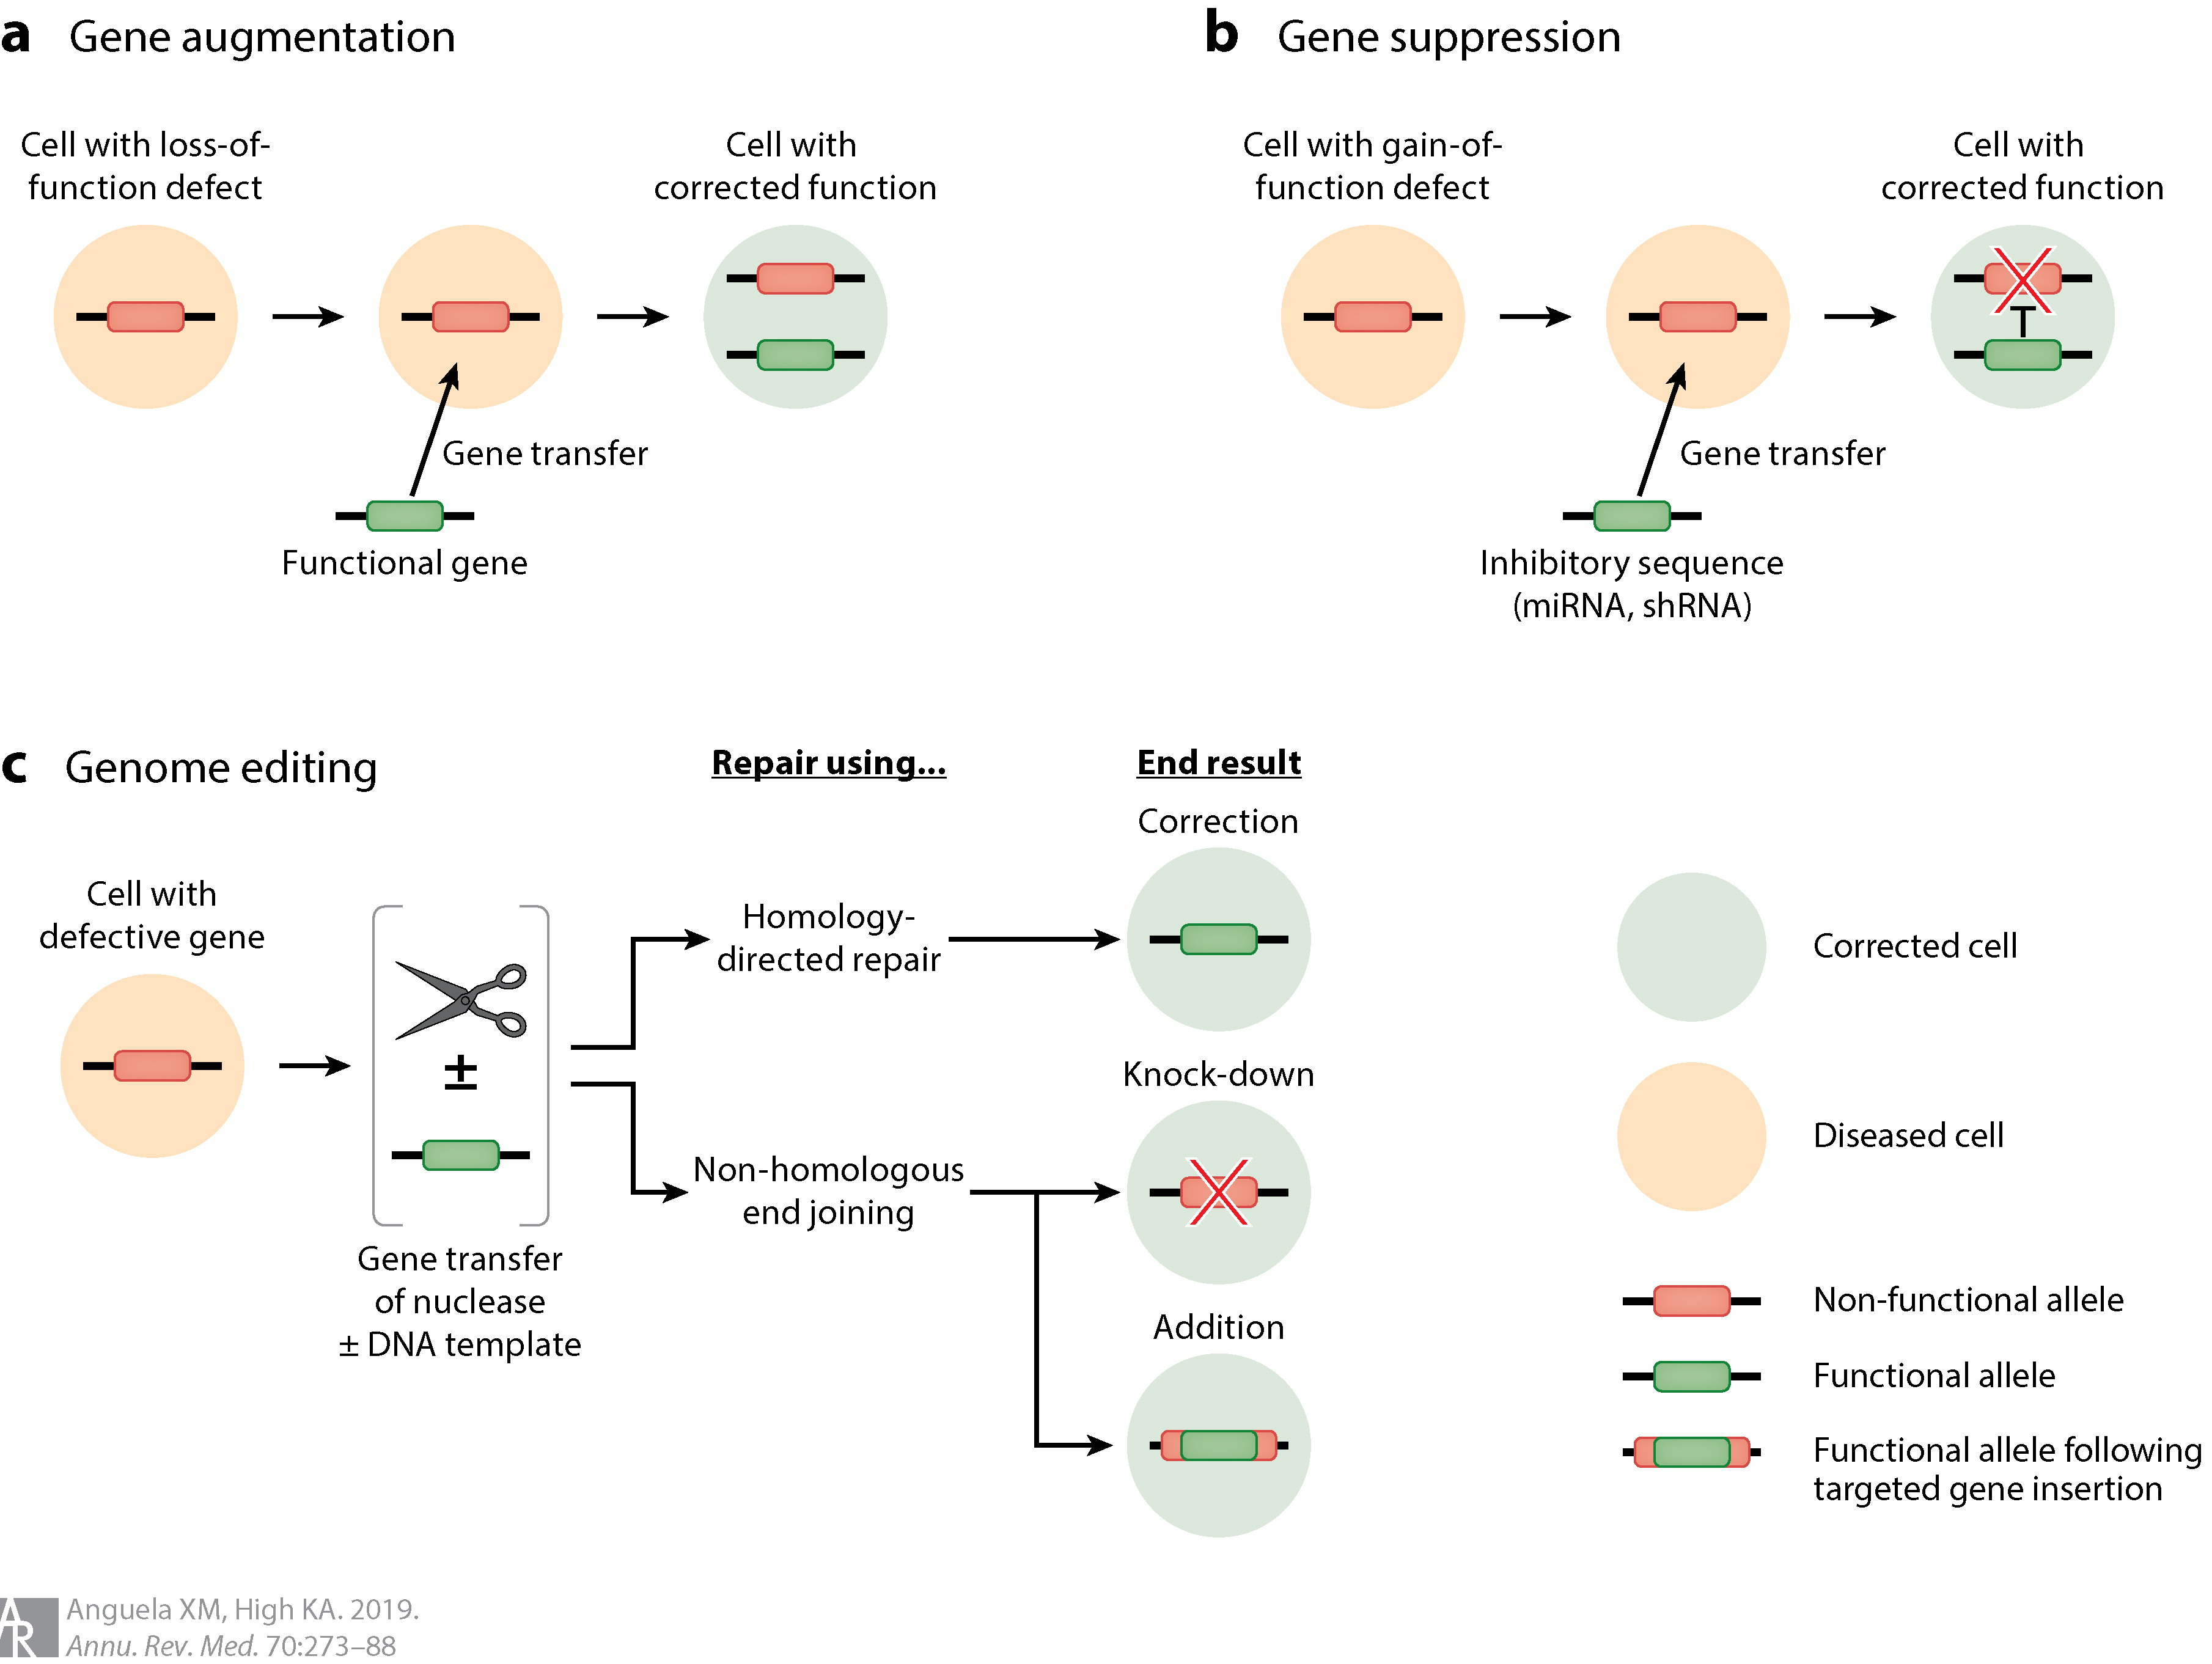
\includegraphics[width = 0.9\textwidth]{1introduction/pics/gene_therapy.jpeg}
\caption[Principles of gene therapy]{Principles of gene therapy. Reproduced from \cite{Anguela2019}.} \label{fig:gene_therapy}
\end{center}
\end{figure}

Augmentation gene therapy introduces an healthy gene copy to restore the normal functionalities of the protein of interest and thus of the cell: it usually consists in the delivery of a DNA strand, which in turn can be internalised in the genome and thus spread when the cell replicates, or not internalised and thus can influence the functionalities of the particular transfected cells only.
%
Suppression gene therapy suppresses a detrimental gene, and this is particularly useful in the case of cancer, to impede cancer cells replication. Usually this strategy employs RNA interference, delivering miRNA (microRNA) or siRNA (small interfering RNA) strands which repress the transcription of the problematic RNA sequence.
%
Finally, gene-editing, the most recent advance in the field, overlooks the possibility of correcting base pairs mutations to restore the original healthy sequence, and is often done through the functionalisation of the CRISPR-Cas9 technology, a mechanism found in prokaryotic organism as defence against viruses \cite{Barrangou2015}:
%
CRISPS (clustered regularly interspaced short palindromic repeats) is a library of DNA fragments from viruses that have previously infected the prokaryote, and the Cas9 enzyme (``CRISPR-associated protein 9") uses these sequences to recognize and cleave strands of DNA complementary to the CRISPR sequence to blocks the reproduction of viruses if a following infection occurs. Research has been able to engineer the CRISPR-Cas9 technology to edit (rather than simply cleave) genes within eukaryotic organisms \cite{Zhang2014cas}, thus performing a therapeutic role.

Despite the challenge posed by the development of genome editing tools, and the risk associated to them (for example the possibility of deleterious insertional mutagenesis or deleterious immune responses), at present six gene therapies have received approval in the Western world \cite{Anguela2019}, with many more undergoing regulatory review. 

One of the main challenges in the development of such therapies lies in the identification of a suitable vector: delivery of free genome in solution results in poor internalisation and low therapeutic effect. Vectors instead allow the DNA/RNA to enter effectively into the cell: viruses can be used, modifying their genome to include the necessary sequence and remove the ones promoting viral replication \cite{Naldini2011,Mingozzi2011}.
%
But nowadays the outlook of gene therapy research lies not only in improving specific cargos to cure at the molecular lever more diseases, but also in the research of appropriate vectors with low toxicity, low induced immune response and high delivery efficiency. In that respect synthetic vectors started to be investigated for a virus-free delivery strategy. The system studied in this thesis proposes, among its other functions, to deliver genetic material into human cells.


\section{Delivery of therapeutic material}
The problem of gene delivery sets a parallel with the small drug one, introduced at the beginning of the chapter. Indeed small molecules needs delivering agents to be efficiently internalised in the cells, as well as genes do.

To reach the aimed organ, therapeutic molecules must be compatible with the different cellular environments they cross, but be preferentially retained, and act only on the ones they are designed for. This implies a subtle balance between a invasive activity on one side, and mimesis on the other, least the compound is recognised as dangerous and disposed by the immune and reticuloendothelial systems.

As en example, the trip of a standard, orally administered drug, passes through the digestive system, with its challenging acidic environment and limited permeation across the intestinal epithelium, and from there to the blood stream \cite{Masaoka2006, Mitragotri2014}. 
%
At this point, the drug is generally coated by a protein corona based on the molecule shape and charge \cite{Krol2012}. The nature of this coating is difficult to predict and can disrupt or decrease significantly the efficacy of a compound as it modifies the way it is recognised and absorbed.
%
From the blood the drug diffuses in the tissues flanking the blood vessels naturally depleting its concentration downstream \cite{Krol2012}, so that regions further away in the line have less chances of getting a sizeable dose. 
%
Moreover, specific tissues are highly impermeable: the blood brain barrier (BBB) for example allows the passage only of small molecules with high lipid solubility \cite{Pattni2015, Krol2012}; while tumoural tissues are instead poorly vasculated, reducing the chances of delivery at their interior \cite{Pattni2015}.

For all the above reasons, research has focussed on developing systems to assist the delivery of drugs. A mimetic carrier can not only improve delivery, but also be designed to selectively bind to particular tissues, or to trigger a drug release delayed time, or release it upon changes in environmental variables (for example pH) to reduce drug concentration in non targeted regions. A stand alone field of research has then focussed on the development of delivery vehicles irrespective from the quest for new drugs. The optimised products of the two separate efforts can then be paired according to the condition to address, to give a successful therapy.

At present, many molecules have been successfully employed to build drug vehicles, both organic and inorganic, to offer a range of different physico-chemical characteristics useful to target different cells \cite{Hughes2005} (Figure \ref{fig:vehicles}). We briefly list them to point out the variety and exoticity of structures which are useful, sometimes unexpectedly, to the medical world, and we then focus on a particular class, peptidic delivery vehicles: once more this class of molecule can offer a  solution to a therapy-related task.

\paragraph{Inorganic materials for small drugs delivery}

\begin{figure}
\begin{center}
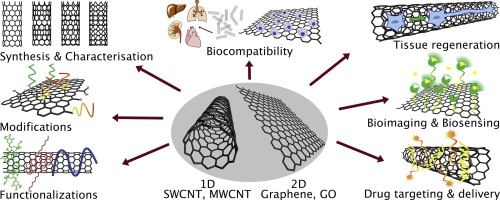
\includegraphics[width = 0.5\textwidth]{1introduction/pics/carbon_review.jpg}
\vspace{0.2cm}
\caption[Materials for drug delivery vehicles]{INCLUDE ONE EXAMPLE IMAGE (FROM PAPERS) FOR EACH MATERIAL (nanopartcles, carbon, polymers, lipids, DNA, proteins).} \label{fig:vehicles}
\end{center}
\end{figure}

Many inorganic compounds have been used to transport drugs or to enhance their biocompatibility. A first class is constituted by metal nanoparticles, with golden nanoparticles covering a major role. Thanks to their metallic nature, these materials can be customised in shape and size (down to a 10 nm radius), and possess optical properties that allow to track them inside the body or to thermally stimulate them to trigger drug release \cite{Boisselier2009}. They can also be coated with biologically active moieties to enhance their mimesis \cite{Singh2018}. For these reasons, they are used to selectively treat tumoural cells, but up to now only a few golden nanoparticle based compounds have made to the clinical stage so far, as there are mixed evidence about their toxicity \cite{Boisselier2009}. 

Similarly, materials made from carbon, especially carbon nanotubes, can be used for biomedical applications as they have a high loading efficiency thanks to the high surface area and easy interaction with biomolecules through van der Waals forces, $\pi$-$\pi$ stacking or hydrophobic effect \cite{Erol2017}. They can be conjugated to extra organic groups to increase their biocompatibility and have potential for targeted drug release upon change in environmental pH \cite{Depan2011}.

Finally polymers are a class of inorganic molecules already well validated as drug eccipients. The most notable example is Polyethylene glycol (PEG): thanks to its high hydrophilicity, it is widely used to coat structures (e.g.\ inorganic nanoparticles, peptides) which in turn carry a drug \cite{Lammers2009}; or as a stand alone carrier system with high drug payload \cite{Liechty2010}. The great strength of polymers is their flexibility: as each of their constituent monomers can be either hydrophilic or hydrophobic, they can be engineered to assemble in many different structures, to swell slowly in water triggering a sustained drug release \cite{Nicolas2013}, or to undergo sol-gel phase transition upon specific changes in the environment \cite{Liechty2010}.


\paragraph{Organic materials for delivery: lipids and DNA} \label{sec:organic}

A somehow opposite approach for designing drug vehicles consists in using molecules similar to the ones present in the body, in an effort to exploit already available biocompatible materials and reduce toxicity \cite{Yoo2011}. In this category fall lipids, DNA and peptides.

A great variety of lipids is present in the cell membrane, and this is further enlarged by the production of synthetic ones. The components selected for drug delivery are usually taken from the biological lipidome, modifying the composition and possibly including synthetic molecules to tune the release and robustness to degradation \cite{Yingchoncharoen2016}.
%
Being amphiphatic, lipids can encapsulate efficiently both hydrophobic or hydrophilic drugs, arranging respectively in micelles (monolayer spheres with the hydrophobic tails facing the interior) or in liposomes (bilayer spheres with a water filled core) \cite{Bunker2016}, and by now, many lipids are approved as delivery agents for cancer and infection drugs \cite{Pattni2015paper, Jain2017}.

DNA scaffolds are instead a more novel tool: DNA origami is nowadays an established technique to build three dimensional customised solids \cite{Linko2015}, and the nanometric knowledge about their constituents allows to fine tune them for a triggered release of the content \cite{Douglas2012}. First studies proved them successful in delivering anticancer agents \cite{Zhang2014, Jiang2012}, however they are very sensitive to different cellular environments which challenge their stability. This, united with high production costs and the relative young developments in their manipulation, prevented them to constitute a viable class of carriers so far, but at the same time holds promise for future improvements and applications.


\paragraph{Peptidic scaffolds} Another widely used and trustworthy mimetic vehicle comes, quite surprisingly, from the world of pathogens: viruses have co-evolved with humans, to be able to penetrate into cells where they complete their reproductive cycle \cite{Lobo2009}. Therefore their capsid, the peptidic shell encapsulating the genome, is highly suitable for cell penetration. The first application sought historically was to employ genome free viruses to stimulate and train the natural immune response against the respective genome-loaded ones, creating viral vaccines - in a concept similar to the inoculation of dead bacteria to counteract the infections caused from them \cite{Lauer2017}.
Later in the history, their potential as cargo carrier was pursued by first modifying the original genetic material to include sequences beneficial for the host cell, and inactivate the ones promoting the infectious duplication at the same time. In particular adeno-associated virus (AAV) has been widely studied \cite{Daya2008} as it triggers a low immune response.
%
To fully exploit the potential of a peptidic carrier many efforts have focussed on synthesising in vitro gene-free capsids, either as they appear in nature \cite{Wu2009} or designing artificial building blocks, which assemble in so called Virus-Like particles (VLPs). This helps overcoming the reaction stimulated by specific viral capsids to which the immune system is sensible to.
%
Similarly to other delivery vehicles, the surface of VLPs can be functionalised with additional molecules to improve the target selectivity and increase biocompatibility, while the capsid peptidic scaffold grants robustness to the structure. Therefore, VLPs loaded with drugs can be tuned for an efficient intra cellular release \cite{Ma2012}.

A step further in engineering peptidic structures is represented by the design of self-assembling functional structures from first principles, exploiting the physico-chemical characteristics of peptides, regardless their resemblance of viral capsids.
%
Indeed, self-assembling peptides can form nanostructures ranging from nanoparticles to nanotubes, nanofibers, nanorods and hydrogels \cite{Fan2017}.
%
Among their advantages, peptides present biocompatibility, a low production cost and a tunable bioactivity thanks to their chemical diversity, which helps in tailor the assembly toward the target of interest \cite{Fan2017}. Moreover, the variety of amino acid available makes possible to load peptidic structures with both hydrophilic and hydrophobic drugs, according to their amino acid composition \cite{Ma2012}.
%
The peptidic self-assembly is modulated by the peptide length and its hydrophobic or hydrophilic character, given by its amino acid composition: simple phenylalanine dipeptides were designed with inspiration from a pathogenic pathway of molecular self-assembly and were shown to self-assemble in a multi-scale process producing nanotubes able to load drug molecules \cite{Silva2013}. The relatively small diphenylalanine building block is non the less complex as it bears two charged termini (as the process is observed at neutral pH), and two aromatic hydrophobic rings, so that the dipeptide is driven towards assembly by the hydrophobic forces acting on the phenylalanine side chains and the complementary charges of the termini.

In a different approach, longer sequences can be employed to guide the formation of the local structure, as they organise spatially in well studied secondary structures with known interactions among themselves.
%
This knowledge is possible as proteins are a fundamental component of the human body and as such an updated database of their structure is available (the Protein Data Bank \cite{PDB}) and can be queried to understand how small peptides hierarchically assemble into larger units.
%
Moreover, the vast literature on their interactions with membranes, cell receptors and in general biological components, can inspire the design of building blocks sensible to particular triggers within the body. From this background, the outlook of protein design often goes in the direction of surpassing natural limitations, synthesising exotic, non natural, geometries \cite{Yeates2019,Malay2019} for multifunctional materials.


\section{Closing the circle: an antimicrobial drug delivery vehicle}

Twice in this introduction peptide design has been brought to the reader's attention. First, it can produce antimicrobial peptides with improved potency or selectivity, or reduced toxicity. Second,  design can engineer self-assembling building blocks for the formation of delivery scaffolds. As design is not bound to natural rules, it can foresee and imagine multifunctional materials which are not observed in nature. In particular, the introduction above poses the question of whether it is possible to engineer peptides able to perform both an antimicrobial and a delivery function at once (either of drugs or genetic material).
%Thus, the relevance of such compound would be twofold.

Such self-assembling, antimicrobial compounds would have a twofold interest for medical applications.
%
First of all, self-assembly is functional to the antimicrobial activity: many AMP sequences have a weak potency, and only a high (critical) concentration can trigger the bactericidal mechanism. This is intuitive in the case of the carpet model strategy (see Section \ref{AMP_mechs}), where AMPs lay homogeneously on the surface of the bacterial membrane and breaks it upon sufficient coverage of its area. Also the barrel-stave and toroidal pore models rely on the mutual interactions between peptides to maintain the pore edges.
%
Generally, as AMPs are positively charged, the localised presence of many copies of a sequence enhances the local electric field and charge imbalance, which are critical to the membrane stability. 
%Thus a self-assembling sequence will enhance the local concentration which is crucial to initiate the membrane disruption.
%
Second, in order for the assembly to be able to perform the additional delivery function, it must be able to either organise in a tailored structure (for example a capsule able to host a drug), rather than an amorphous aggregate, or to co-assemble with the cargo of interest.

Out of all the possible applications, the most promising is perhaps the use of such vehicles to deliver drugs to treat metabolic or genetic diseases: while the cargo tackles a defect of the host system, the vehicle can counteract the proliferation of bacteria. This is particularly important in situation where the host immune response is weakened and thus infections normally harmless can spread and cause damage.
%
However, it must be noticed that the cargo is not bound to be a small molecule, as long as it can effectively co-assemble with the peptidic carrier. As mentioned in the previous section, gene therapy is also an actively expanding field which looks with interested at the development of vehicles for genetic material. Given that viruses have been the first choice for DNA/RNA delivery so far, peptidic carriers seem a natural evolution of them.

\bigskip
Given the above premises, it is evident the importance of pursuing the research on novel multifunctional peptidic materials.
As mentioned when discussing AMPs design, to understand such systems, each of them must be characterised by itself, as a generalised knowledge is still lacking.
With this aim, this thesis proposes to elucidate the behaviour of a specific synthetic self-assembling peptide, suitable for antimicrobial activity and gene delivery strategies. Its full characterisation will complete the knowledge on its mechanisms of action and complement the broader information already known on the class of such functional building blocks. This will be crucial to engineer new synthetic blocks with improved characteristics, either regard their antimicrobial activity, assembly performances, or tailored cargo delivery.


\subsection{Capzip} \label{sec:capzip}

\begin{figure}
\begin{center}
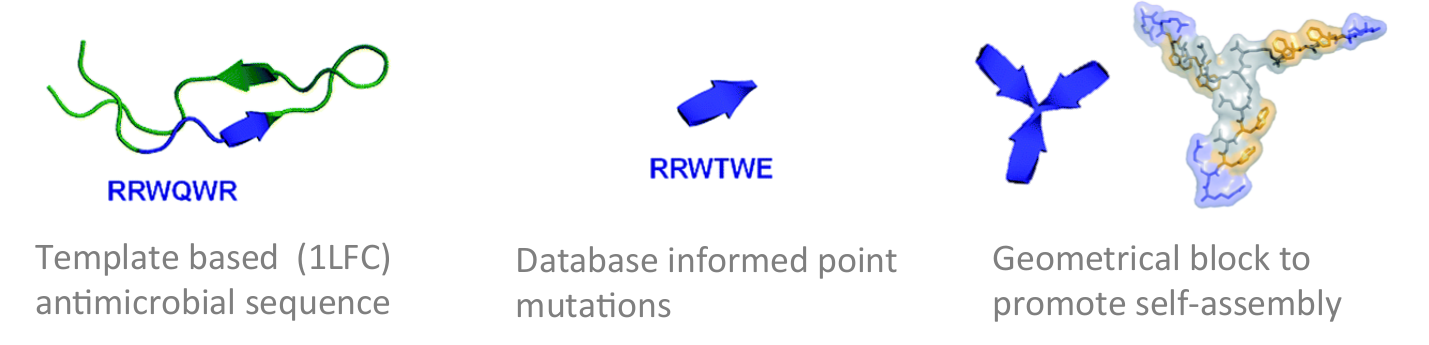
\includegraphics[width = \textwidth]{1introduction/pics/capzip.png}
\caption[Cazip molecule]{Capzip molecule scheme and bond representation. [TO BE IMPROVED] Adapted from \cite{Castelletto2016}.} \label{fig:capzip}
\end{center}
\end{figure}

The molecule capzip has been designed to perform the functions mentioned above at once. To recapitulate, the properties it possesses are:
\begin{enumerate}
\item assembly into nanoscale virus-like capsules with and without nucleic acids. This ensures that the vector can autonomously form and thus there is flexibility in the choice of the cargo;
\item antimicrobial activity of the molecule itself and of the capsule on a time scale useful for therapeutic applications;
\item promotion of gene transfer into mammalian cells when the peptide is co-assembled with the RNA strands, without causing cytotoxic and haemolytic effects.
\end{enumerate}
%
Furthermore, the design effort aimed at building a template structure of minimal complexity, in order to reduce the synthesis effort to a short sequence. Arguably, short sequences are also more flexible in their assembly: it is thus important to explore them and prove whether even small blocks can form ordered structures.

Based on the above requirements, two design principles emerged: first the employment of a non-linear structure. There is indeed some evidence suggesting that non linear peptides are more prone to assemble in three dimensional structures, opposed to planar ones \cite{???}, and this holds in particular for short sequences which do not fold into a defined secondary structure.
%
The second principle consists in the use of a template antimicrobial sequence which is short and has proved potency.
%
Given that AMPs are usually anionic, the co-assembly with anionic RNA sequences is arguably inherited by consequence.

To satisfy the above guidelines, a short peptidic scaffold constituted by a $\beta$-Alanine and two Lysins has been engineered.
%
Three identical copies of the antimicrobial sequence of choice are covalently bonded to the N-terminus of the scaffold sequence and to the nitrogen atom of the Lysin residues side chains (Figure \ref{fig:capzip}).
%
Regarding the antimicrobial sequence selected, it has been derived from the antimicrobial peptide bovine lactoferricin, which is in turn a portion of the Lactoferrin protein.

\paragraph{Lactoferrin} Lactoferrin is an iron binding protein present in milk (in which it is most abundant, hence its name), saliva and other secretions, as well as in polymorphonuclear leukocytes.
%
It works as an iron binder and provides a natural defence against bacteria and fungi \cite{Sanchez1992,Arnold1977,Arnold1980,Kirkpatrick1971,Jahani2015}, constituting a first defence for infants.

Lactoferrin contributes to bacterial suppression in several ways. At present, its known modes of action fall in three categories: first, thanks to its iron sequestering capabilities, it removes essential substrate required for bacterial growth \cite{Farnaud2003}; second, it interacts with bacterial membranes and in particular binds to the lipopolysaccharides of bacterial walls, oxidising them and affecting the membrane permeability with consequent cell lysis \cite{Farnaud2003}; finally it is implicated in the stimulation of different immunological cells (killer cells \cite{Shau1992}, polymorphonuclear leukocytes, and macrophages \cite{Gahr1991}).
The peptide fragment responsible for binding of lactoferrin to the bacterial membrane, named lactoferricin (Lfcin), has been identified near its N-terminus and found to have a more potent bactericidal effect than intact lactoferrin on a wide range of bacteria \cite{Gifford2005,Bellamy1992,Tomita1994,Wakabayashi1996}.
%
Similarly, a synthetic short peptide derived from a subsequence of human lactoferricin has been proven effective against bacteria as it depolarises the cytoplasmic membrane decreasing the pH gradient \cite{Aguilera1999}.

The bovine homolog of lactoferricin (LfcinB) has a higher bactericidal potency than human lactoferricin on several bacteria \cite{Cochran2001} and therefore has been more extensively studied. Its active core LFC is a 25-amino acid sequence which adopts a helical conformation in the full structure but, once isolated, crystallises in a $\beta$-hairpin with a disulfite bridge nearby the terminals which stabilises the fold, but was shown to be not essential for bactericidal activity \cite{Cochran2001}.
%
Further experiments on LfcinB subsequences identified an even shorter antimicrobial core, constituted by the six amino acids RRWQWR \cite{Schibli1999}. This core presents a characteristic Tryptophan zipper motif WTW, which appears very often in nature in $\beta$-turn and $\beta$-sheet conformations, paired to another copy of the same motif, so that Tryptophan rings from facing strands are packed tightly against each other in an alternated way \cite{Cochran2001} (Figure --).
In general, the six amino acid sequence contains both charged and hydrophobic residues, in line with the usual composition of antimicrobial peptides. Accordingly, its antimicrobial action is likely derived from the interaction with biological membranes through charge recognition first and aromatic rings insertion in a second moment.

To further elucidate this mechanism, several experimental investigations have been carried both on LfcinB and its subsequences. First, the structure of LfcinB in solution has been investigated by NMR (Nuclear Magnetic Resonance), resulting very flexible \cite{Hwang1998}. Then, the binding of its antimicrobial core to sodium dodecyl-sulfate micelles was studied \cite{Schibli1999}, suggesting a favourable interaction of aromatic residues with the micelles surface.
%
Similar experiments were performed on large unilamellar vesicles, constituted by lipids modelling biological membranes: ePE:ePC was chosen as a model of a mammal membrane, and ePE:ePG or ePC:ePG for a bacterial one. The experiments showed preferential binding to the latter ones, based on Tryptophan fluorescence \cite{Nguyen2005}, suggesting a selective antimicrobial action on anionic membranes.
%
Additional experiments have been performed on the full sequence or mutated subsequences \cite{Tsutsumi2012,Arseneault2010} to investigate the binding to other different model membranes but, as the systems investigated are slightly different, as well as the experimental conditions, it is difficult to relate them and give a unified interpretation of the modes of action of lactoferricin derived peptides.

Finally, an alanine scanning has attempted to clarify the role of each amino acid in the antimicrobial activity of the LFC peptide \cite{Strom2002}. The results suggested a binding function for the Tryptophan residues, in line with one of the roles Tryptophan can assume in antimicrobial peptides \cite{Chan2006}. Other possible roles involve its propensity to form hydrogen bonds, in which case the residue would position itself at the interface between solution and membrane, rather than inside the latter (which happens instead when Tryptophan residues have a binding role).

\paragraph{The designed block}
From the active core of LFC (of sequence RRWQWR), a mutated sequence was obtained to comply the design criteria of a self-assembling building block. Two mutations were introduced to favour the assembly of arms belonging to different molecules in an antiparallel fashion. Specifically, given that the original RRWQWR sequence is found in a $\beta$-sheet (at least in the crystal lattice), the mutations aim at promoting a similar structure. Therefore, the Glutamine residue and the C-terminal Arginine of the lactoferrin motif were replaced with Threonine and Glutammic acid residues to have a self-complementary sequence RRWTWE: the pairing is promoted by the attraction of opposite charges at the ends of the sequence.
%
Three copies of this sequence were thus covalently bonded to the scaffold described previously and shown in Figure \ref{fig:capzip}, to obtain a self-assembling molecule in a three dimensional shape, hosting multiple copies of an actively antibacterial sequence.

%With the virus architecture adopting an n-fold rotational symmetry, where n is usually 3 or 5 or both,9 a triskel conjugate of RRWTWE was generated to give a self-assembling motif with a trilateral symmetry reminiscent of native cage-like subunits (Fig. 1b–e and S1 in ESI†).

\subsection{A viable systems: experimental background and question}
Many experiments have been performed to verify that capzip had the characteristics it was designed for. The set of experimental results obtained on the molecule has been published in Reference \cite{Castelletto2016}, while more recent results extend and consolidate the previous findings.

\begin{figure}
\begin{center}
\textbf{AFM/TEM \ \ \ \ \ \ \ \ \ \ \ \ \ \ cryo-em}
%\subcaption{}\label{fig:exp_capzip_a}
%\subcaption{} \label{fig:exp_capzip_b}
\bigskip

\textbf{fluo hollow capsule \ \ \ \ \ \ \ fluo RNA uptake}
%\subcaption{} \label{fig:exp_capzip_c}
%\subcaption{} \label{fig:exp_capzip_d}
\caption[Experimental results on capzip]{... Reproduced from \cite{Castelletto2016}} \label{fig:exp_capzip}
\end{center}
\end{figure}

\paragraph{Experimental results} First, the assembly ability have been tested: the peptide does not show assembly in pure water (as verified by Dynamic Light Scattering), while in biological buffer (MOPS, 150 mM) at physiological pH of 7.0 it forms capsules with dominating size range of 20-200 nm. This is confirmed by images of the capsules obtained with multiple techniques, namely transmission electron microscopy (TEM) (Figure \ref{fig:exp_capzip}), atomic force microscopy (AFM), and cryo-scanning electron microscopy (SEM).
%
The fine structure of these assemblies appears irregular to the resolution power of such techniques. Some insight into the details of the assembly is given by Circular Dichroism (CD) spectra, which show a profile characteristic of $\beta$-turns and contain elements of a $\beta$-sheet structure and of indole rings, with minima at $\lambda \sim$ 200 nm and 214 nm.
%
Complementary evidence about the overall shape of the assembly was provided by the cross-sectional analysis of the assembled capsules by fluorescence microscopy using fluorescein to label capzip. The signal comes from the wall of the capsule only, showing an inner cavity (Figure \ref{fig:exp_capzip}).
%
Finally, small angle X-ray scattering (SAXS) measurements were consistent with compact capsules interfacing with solvent.

The assembly process is also tested and monitored in combination with small interfering RNAs (siRNA): as mentioned in section \ref{sec:gene_th}, these sequences are a promising tools for RNA interference techniques which aim at inhibiting the expression of specific genes, however, they are easily degradable and thus difficult to deliver to the target cell without an appropriate vehicle.
%
The co-assembly of a 21 base pairs duplex with the peptide shows the formation of structures similar to the ones formed by the stand alone peptide only: CD spectra highlight the helical signal from RNA together with the features proper of the peptide.

These co-assembled structures were tested for siRNA delivery in HeLa cells, showing that the presence of the peptide favours the internalisation of the genetic material with respect to the transfection results of a pure siRNA control. The delivery of fluorescent siRNA (Figure \ref{fig:exp_capzip}) showed that the internalisation occurred within the first hours from the transfection in localised regions of the cytoplasm, suggesting an endocytic uptake. This distribution was stable over the first five hours of incubation after which the fluorescence signal decayed.
%
Flow cytometry assays quantified the increase in siRNA uptake levels due to the presence of capzip, confirming that this molecule is competitive with other commercial transfection reagents (like Lipofectamine\textsuperscript{\textregistered}, unpublished results).

To further quantify the level of RNA internalisation, a mRNA knockdown experiment was performed on a HeLa cell line with two housekeeping genes, ACTB ($\beta$-actin, targeted) and GAPDH (reference) \cite{Crombez2009}.
%
The silencing of $\beta$-actin mRNA was detected 22 $\pm$ 2 hours after transfection; and its knockdown ``fitness" was expressed relative to cells treated with siRNA alone (background) and normalised against viable cell counts (Figure \ref{fig:exp_capzip}). Capzip fitness was lower than Lipofectamine\textsuperscript{\textregistered} one, however cells treated with capzip remained viable after 24 or 48 hour, resulting in higher cell counts than the samples treated with the commercial reagent, suggesting that capzip has little cytotoxicity.
%
The experiment above was performed at neutral to positive charge ratio close to one (where each siRNA molecule has a -42$\, e$ charge and capzip a +6$\, e$ charge), as test experiments performed at higher peptide-to-siRNA ratio showed no improved uptake.

Finally, the peptide does exert an antimicrobial function: the non-assembled peptide has shown to be effective against both Gram positive and negative bacteria (E. coli, P. aeruginosa and S. aureus), with no haemolytic effects and minimum inhibitory concentrations typical of other antimicrobial agents.
%
On Supported Lipid Bilayer with negative total charge (mixed DLPC and DLPG, 3:1 ratio), the capsules create localized pores within minutes, as proven by AFM experiments repeated in time. The pore depth ranges between 1.4 and 2.2 nm, which is smaller than the radii of the capsules, however it is sufficient to disrupt the structure of the membrane.
%
Finally, to prove the viability of capzip as antimicrobial agent in vivo, it was used to counteract methicillin-resistant S. aureus (MRSA) infections in G. mellonella larvae. The particular bacterial strain used was susceptible to vancomycin, which could be used as control: the larvae treated with capzip showed survival rates significantly higher than the untreated control, and comparable to those treated with high doses of vancomycin (unpublished results).

%MANCA: microfluidic results

\paragraph{Open questions} Despite the success of the experiments mentioned above, there is much information still to be uncovered on the precise mechanism of action of such peptide. 

Specifically, both the assembly process and the antimicrobial mechanisms contain some unknown: regarding the former, it is important to understand which amino acids or sub-structures allow the pairing of molecules, whether such pairing is specific or not, how reversible it is, and how rigid the final structure is.
%
Regarding the latter, it must be highlighted what molecules in the membrane the peptide binds to, and how this binding affects the full membrane structure. Finally, as there is evidence that the assembled molecule is a more powerful antimicrobial compound than the single molecule, it is interesting to understand whether any cooperative action is taking place or the enhanced antimicrobial power of the assembly is due only to the localised higher concentration.

Even if further experiments or future improvements in the techniques already employed might tackle some of the aspects above in a near future, arguably no experimental outcome can provide an atom-by-atom knowledge of the processes of interest in any time soon. Ideally though, one would like to track each of them, i.e. the processes happening in any the environments capzip has been exposed to (physiological solution, supported lipid bilayers, bacterial extracellular matrix, mammal cell membrane and cytoplasm) both in space and time with the finest level of details, and the impossibility of that leaves large gaps in the understanding of the system.


\section{A computational approach to understand capzip}

The gaps mentioned in the characterisation of the systems prompts for new investigations in order to complement the knowledge already provided.

Beside the quest to enrich the fundamental knowledge on self-assembling peptides and antimicrobial ones, the understanding of this very system is crucial for its further development. We outlined already in Section \ref{sec:amp_design} how antimicrobial peptide design can proceed from already viable templates and empirical principles, when first principles are not available. Similar rules hold for designing self-assembling peptidic materials, to obtained tailored delivery vehicles (see Section \ref{sec:organic}).
%
Therefore, a full knowledge of the interactions between peptides and between their assembled structures and the membrane, i.e.\ of the mechanism of its functions, will drive the engineering of new likewise peptides. A knowledge-driven design would hopefully provide new blocks suitable for a double action as the one capzip performs, and this in a shorter amount of time than a research based on less information or on a trial-and-error procedure of mutations in the chemical composition or in the architecture of the molecule. A few examples of possible knowledge-related improvements include the following:
\begin{itemize}
\item the knowledge of capzip binding mode to the bacterial membrane might suggest its suitability as a broad range spectrum compound or the possibility of tuning its action against specific pathogens;
\item understanding the molecule-molecule interactions classifies the robustness of the assembled structure and the possibility of designing block which disrupts under particular chemical conditions only;
\item querying the electrostatic profile of the assembled structure suggests which type of molecules, other than siRNA, could be efficiently co-assembled and thus delivered.
\end{itemize}

In recent years, computational techniques are stepping forward to complement incomplete experimental knowledge and complete the picture of how biological systems work. For this reason, it seems natural to query such techniques to study the capzip system as well. Zooming into the details of the interactions can be performed via a theoretical modelling of the system in time, and thus through the simulation of its evolution, starting from few basic principles and the knowledge of the chemical composition of its parts. The technique this work focusses on is Molecular Dynamics simulations, which aims at reproducing the behaviour of a system of atoms in a semi-classical description using basic physical laws, as it will be described in details in the next chapter.

Thus it is the aim of this thesis to prove that Molecular Dynamics simulations can clarify further details on the assembly mechanisms of capzip and on its interactions with biological membranes, in order to gather more information on the system and contribute in the future to the designed of new molecules with enhanced functional capabilities.

%MORE SPECIFIC QUESTIONS

%\paragraph{Bits}

%In the triskel conjugate, RRWTWE is prone to fold as a b-turn and pair into a b-sheet with another arm of another conjugate.7 Triskelions are then
%compact globular morphology of the capsules observed by AFM in solution (Fig. S3†). 

%The specificity of these antibiotics allows generally to selectively target the desire species of bacteria, however it has the drawback that small modification in the target can easily invalidate the effect of the drug. 

%The typical time at which this resilient population appears varies greatly according to the mechanism targeted by the drug, but also and especially by how this is administered, resulting in the modern ways of treating infections a particularly fertile ground to train drug-resistant bacteria. Key reasons of the acceleration of the mechanism are the more extensive - and sometimes unjustified - use of antibiotics, both in the doses used for patients and in the world wide coverage that nowadays can, luckily, been reached. It must not be forgotten that a large portion, if not the majority, of antibiotics do not come from human treatments but actually from agriculture and breeding.
%
%This increased pressure allow for a fast spread of resistance, but the emergency comes from the parallel lack of new discoveries of novel drugs. The few discovered and approve are kept as last resources and used carefully, both to prevent insurgence of resistance as long as possible and for their collateral effects: indeed, the inefficacy of other drugs has pushed pharmaceutical industry to resort to compounds discarded in the first screening because too toxic for the human body.

%The design of new synthetic AMPs can enhance the self-assembly property to improve the antimicrobial activity and to tailor the final structure into an organized geometry suitable as delivery vehicle \cite{Wei2017, King2014, Norn2016, Korendovych2010, Vauthey2002}.
%The design procedure must necessarily be directed by means of both experimental and theoretical modelling techniques \cite{Fjell2011, Maccari2013, Zhang2015}. Indeed, in silico techniques help to evaluate the physico-chemical characteristics of novel compounds and select the sequences suitable for the purpose. Additionally, they can elucidate the mode of actions of the antimicrobial activity which is still unclear for many AMPs, despite the vast body of experiments performed in the field \cite{Nguyen2011, Chan2006, Ulmschneider2017},

%In this context we want to employ computational techniques to investigate the characteristics of a synthetic antimicrobial peptide designed and tested for its self-assembly characteristics. Capzip \cite{Castelletto2016} is a branched peptide which incorporates three copies of a six amino acids AM sequences (one for each branch, SI Figure \ref{fig:SI_capzip_formula}).
%The sequence (RRWTWE) is a mutation of the antimicrobial region RRWQWR of the bovine lactoferricin peptide (PDB entry 1LFC)\cite{Schibli1999}. The mutations have been introduced to create a self-complementary sequence prone to antiparallel $\beta$-sheet formation with other identical sequences belonging to different molecules, via pairing of opposite charges \cite{Castelletto2016}. The three branches enforce a 3-fold rotational symmetry, reminiscent of the architecture of viral subunits, which aims at generating a three dimensional self-assembling motif, as the branches lies onto different planes.

%One of the key advantages of AMPs over pharmaceutical antibiotics is the ability of some of these peptides to also modulate immune responses. For example, in addition to their direct antimicrobial activity, AMPs can protect the host by a range of mechanisms: chemotactic activity, attracting leukocytes; modulation of host-cell responsiveness to TLR ligands; stimulation of angiogenesi enhancement of leukocyte/monocyte activation and differentiation; and modulation of the expression of proinfl ammatory cytokines/chemokines (Figure 1). For example, LL37 has been shown to attract neutrophils, monocytes, mast cells and T cells. Different groups of AMPs appear to have distinct chemotactic activities from each other. 
%Indeed, a common feature across most of them is the targeting of the bacterial membrane, generally in an unspecific way: membranes of different bacteria share often common characteristics, with all their species classifiable in two groups (Gram positive or negative) according to their membrane(s) structure, and thus AMPs are often effective on many representative of one class, if not both.

%Modification of AMPs with Covalent Bonds,  Modification of AMPs by Changing Amino Acid Content, Modification of AMPs by Amidation, Modification of AMPs with Unnatural Amino Acids, Modification of AMPs with Computer-Assisted Methods, New AMP Design by Homology Modeling

%torres: determining structure-activity relationships. site-directed mutagenesis, computationaldesign approaches, synthetic libraries, template-assisted methodologies, and mechanism-based strat-egies. 

%Gandhi2014 for nanocarrier for siRNA/miRNA

%Joo2016 Andersson2016 AMR to AMPs

%approved peptidic drugs Usmani2017 they are 884
%Recent advances cell-penetrating peptide-assisted drug delivery Langel2015
%Designing improved active peptides for therapeutic approaches against infectious diseases Gomes2018 READ

%Molecular mechanisms of membrane targeting antibiotics Epand2016 READ
%BASIS FOR SELECTIVITY OF CATIONIC ANTIMICROBIAL PEPTIDES FOR BACTERIAL VS MAMMALIAN MEMBRANES 2005Glukhov
%The therapeutic applications of antimicrobial peptides (AMPs): a patent review Kang2017

\chapter{Methods} \label{chapter:MD}

\lettrine{M}{olecular Dynamics} simulations have been rightly defined as the `Computational Microscope' \cite{Lee2009,Dror2012} as they offer otherwise inaccessible insights into the molecular details underlying conformational changes of proteins and nucleic acids. Computational methods and tools based on MD are routinely applied in structural biology to quantitatively characterise the dynamics and thermodynamics of proteins and their complexes. The increasing computational power available, and the flexibility of the algorithms which can be implemented on different platforms, have made possible to access molecular dynamical properties inaccessible to experiments. These techniques and the associated force fields are also commonly used in the process of structure determination from NMR data and theoretical structure prediction \cite{Vogel2017,Heo2018}.

Modelling and simulating a biological system consists in describing its components and their mutual interactions, and implementing the laws of physics in the attempt to reproduce its natural evolution. A quantum mechanic description would be the most accurate but expensive to achieve for large systems. To facilitate the task, several simplified models have been devised, each most suitable to investigate particular cases.
%
In particular, a large class of models focuses on a classical mechanics description of the dynamics: by increasing the size of the systems and with longer time spans described, the classical approximations will become more accurate, and objectively the only possible representation computationally affordable.

We briefly present here the core theory and implementation of classical MD simulations, together with a discussion of their strengths, limitations and comparison with experiments. Understanding their methodology provides the interpretative key with which simulations must be designed, run and interpreted in each specific case \cite{vanGunsteren2006}. A review of relevant successes of MD simulations will complete the chapter.


\section{Algorithms for Molecular Dynamics}

In this section, the core algorithm behind MD simulations is presented, together with the corrections and refinements implemented on it, as it sets the ground for the approximations to follow:
%as much accurately the system can be modelled, in a classical MD framework it will always be processed by an engine based on classical mechanics rules and finite steps approximations, which inevitably influences the outcome.
in classical MD, the system will be processed by an engine based on classical mechanics rules and finite steps approximations, and the forces acting on it can thus be modelled with a similar degree of approximation.

\subsection{The Newton's law}

In the aforementioned framework, Newton's second law of motion rules the dynamics, stating that the acceleration $\textbf{a}$ that a particle is subject to at time $t$, depends on the total force $\textbf{F}$ acting on the particle itself and on its mass $m$ (bold denotes vectorial quantities):
\begin{equation} \label{eq:newton}
\textbf{F}(t) =  m \cdot \textbf{a}(t) \, .
\end{equation}
As the acceleration $\textbf{a}(t)$ is the second derivative of the position $\textbf{r}(t)$ with respect to time, given the initial position and velocity of the particle ($\textbf{r}(t_0)$, $\textbf{v}(t_0)$), their temporal evolution can be computed integrating $\textbf{a}(t) = \textbf{F}(t)/m$ as follow:
\begin{eqnarray} \label{eq:analytical}
\mathbf{v}(t) &=& \mathbf{v}(t_0) + \int_{t_0}^t \frac{\mathbf{F}(t')}{m} \, dt' \, ; \\
\mathbf{r}(t) &=& \mathbf{r}(t_0) + \int_{t_0}^t \mathbf{v}(t') \, dt' + \int_{t_0}^t \int_{t_0}^{t'} \frac{\mathbf{F}(t')}{m} \, dt'' \, dt'\, . \label{eq:analytical2}
\end{eqnarray}
%
In the case of complex biomolecular systems with many particles and multiple interactions acting between them, it is impossible to integrate analytically Equations \ref{eq:analytical}-\ref{eq:analytical2}, while a different and feasible approach consists in discretising them.
%
The idea is to consider very short time steps of length $\Delta t$, so that in such intervals the forces can be considered constant, and the integration of Equations \ref{eq:analytical}-\ref{eq:analytical2} becomes trivial.
%
The simplest choice consists in considering for the integration both the acceleration and the velocity at time $t_0$, producing the Euler algorithm:
\begin{eqnarray} \label{eq:euler}
\mathbf{v}(t_0 + \Delta t) &=& \mathbf{v}(t_0) + \frac{\mathbf{F}(t)}{m} \, \Delta t \,; \\
\mathbf{r}(t_0 + \Delta t) &=& \mathbf{r}(t_0) + \mathbf{v}(t_0) \, \Delta t + \frac{\mathbf{F}(t)}{m} \, \Delta t^2 \,. \label{eq:euler2}
\end{eqnarray}
%
This procedure contains approximation of the order of $(\Delta t)^2$ that will accumulate step after step, biasing greatly the outcome. However, a careful choice of the values to integrate allows to reduce considerably this approximations. For example, choosing the acceleration value at time $t_0$ but the velocity at time $t_0 + \Delta t/2$ decreases the error down to orders of $(\Delta t)^4$. This framework is at the basis of the so-called leap-frog algorithm, which is used in the vast majority of MD engines:
\begin{eqnarray}
\mathbf{v}\left(t_0 + \frac{\Delta t}{2}\right) &=& \mathbf{v}\left(t - \frac{\Delta t}{2}\right) + \frac{\mathbf{F}(t)}{m} \, \Delta t \, ; \\
\mathbf{r}(t_0 + \Delta t) &=& \mathbf{r}(t_0) + \mathbf{v}\left(t_0 + \frac{\Delta t}{2}\right) \, \Delta t \, .
\end{eqnarray}
This algorithm can thus ``solve" every possible Newton equation, at the expenses of some precision.

Considering that MD deals with bonded atoms belonging to multi-atoms molecules, the length of these bonds must be kept within a physically meaningful value. The approximate procedure mentioned above may however give raise to unphysical configurations, even if the forces acting between single atoms tend to bring them in the correct geometry. On the other hand, if the initial configuration was far from equilibrium, very abrupt changes in the bond length can arise in the initial steps, which are unphysical as well.
%
To correct this, constraint algorithms are applied after the update of atoms positions, to limit the change in bond length. The ones used in this work are LINCS (Linear Constraint Solver) \cite{Hess1997} and SETTLE \cite{Miyamoto1992}: the first finds a solution iteratively within an approximation tolerance, as the problem of constraints is hardly solvable analytically; the second is an exact implementation of the solution for rigid bodies of three elements only, and as such is useful for the treatment of water molecules (which have three atoms in their atomistic description).

\subsection{Thermostats and barostats}
As an addition to the geometrical constraints algorithms mentioned above, other specific algorithms have been developed to more realistically reproduce the simulation's conditions of choice, for example Temperature and Pressure.

Most experiments are conducted under constant temperature, so that it is desirable to reproduce this condition in simulations.
%
To set up a temperature, at the beginning of the simulations particles can be given random initial velocities sampled from the Maxwell-Boltzmann distribution, which describe velocities of atoms of a noble gas at temperature $T$. The velocity of each of them will be influenced by the specific interactions occurring in the system but, in a constant temperature environment, the total average kinetic energy (proportional to $T$) must remain constant.
%
Even in absence of any dissipative term in the dynamics, the approximations performed in the MD algorithm make this quantity to drift away from its initial value, therefore to ensure temperature is maintained throughout the simulation, thermostat algorithms have been devised.

The principle behind a thermostat consists in rescaling the velocity of one or few selected particles at fixed interval of times, to restore the correct average kinetic energy. This fixed interval of time must not correspond to the timestep itself, as the goal of a thermostat is to maintain the average temperature, and not its value at all times, as fluctuations are expected in natural systems.
%
Moreover, it is strongly recommended to couple solute and solvent to separate baths, to ensure that both maintain the correct temperature. Indeed, it is possible that the energy exchanged between solute and water (or other components) is not perfect, due to different conditions adopted for their simulations, like, for example, cut-offs or restraints.
%
The most used thermostat algorithms are the Berendsen \cite{Berendsen1984}, Nos\'{e}-Hoover \cite{Nose1983,Hoover1985}, Andersen \cite{Andersen1980} and velocity rescale \cite{Bussi2007}, which differ in the quantities selected for the velocity rescaling.

Another macroscopic condition one wishes to maintain is either the volume or the pressure of the system. While maintaining the volume constant is easy (and, combined with constant temperature, gives the NVT ensemble), pressure regulation (i.e.\ maintaining a NPT ensemble) requires a barostat.
%
Pressure is directly proportional to the average quantity of motion exchanged between the particles and the walls of the box they are confined to, which depends on the frequency of collision and thus on the extent of the box. Barostats change the box size to regulate the pressure.
%
It has to be noticed that most MD simulations are run under periodic boundary conditions, i.e.\ a particle which exits from the simulation box during a move is brought back on the opposite side of the box, leaving the box density constant. This mimics the presence of an infinite number of equivalent boxes one next to the other, and alleviates the finite size effects that arise when simulating small systems.
%
In this scenario, particles are not bouncing on the box walls, rather a virtual pressure is computed from the velocities of the ones trespassing the box boundaries during a move.
%
Similarly as for thermostats, the coupling frequency of barostats must be larger than the time step. Usually all the box dimensions are rescaled by the same amount. However, in the case of anisotropic systems like lipids, to maintain the correct pressure, the directions parallel to the membrane plane can be rescaled separately with respect to the one perpendicular to it.
%
Also for pressure coupling several algorithms can be used: the Berendsen \cite{Berendsen1984}, Parrinello-Rahman \cite{Parrinello1981}, or Martyna-Tuckerman-Tobias-Klein (MTTK) \cite{Martyna1996} (to be used in conjunction with the Nos\'{e}-Hoover thermostat), are all barostats which differ in the way they approach the desired pressure (e.g. exponentially, in an oscillatory way, etc.).


\section{The force field problem} \label{sec:ff}

Once the equations of motion and the control algorithms are set up, the next challenge is represented by modelling the forces and thus the potential energy function.
%
Force fields for classical MD simulations usually rely on the breakdown of interactions into several independent, additive and derivable terms, identified on an empirical physical basis. We report here the functional form adopted for the GROMOS force field \cite{Oostenbrink2004,Schmid2011} as implemented in the GROMACS MD engine \cite{Berendsen1995,Abraham2015,gromacs_man}, as an example of the structure of a classical force field.
%
Other force fields can have slightly different implementations, however the general classification of interactions and the type of functional forms used are similar.

\paragraph{Covalent (bonded) interactions} Covalent interactions are modelled with potential energy terms representing bond stretching, angle bending, improper and proper dihedral angles torsion.
%
The functional form of the potential-energy for bonded interactions aims at a simplified, semi-classical description of the sub atomic motion of molecules, assuming harmonic-like vibrations around the equilibrium position of the bond, angle or dihedral in exam.

Specifically, in the GROMOS force field, a bond between atoms $i$ and $j$ is described by a fourth power potential (similar to a harmonic form, but computationally more efficient):
\begin{eqnarray}
&& V_b(\textbf{r}_{ij}) = \frac{1}{4}\,k^b_{ij}\,\left(|\textbf{r}_{ij}|^2 - b_{ij}^2\right)^2
\end{eqnarray}
where the force constant $k^b_{ij}$ is given in kJ/mol/m$^2$ and $b_{ij}$ is the equilibrium position of the bond between atom $i$ and $j$.

The deviation of the angle between three atoms $i$, $j$ and $k$ from the preferred value $\theta^{\, 0}_{ijk}$ is implemented through a cosine based angle potential:
\begin{eqnarray}
&& V_a(\theta_{ijk}) = \frac{1}{2}\,k^\theta_{ijk}\,\left(\cos\left(\theta_{ijk}\right) - cos\left(\theta^{\, 0}_{ijk}\right)\right)^2 \\
&& \text{with:} \ \cos\left(\theta_{ijk}\right) = \frac{\textbf{r}_{ij}\cdot \textbf{r}_{kj}}{r_{ij}\,r_{kj}}
\end{eqnarray}
with $k^\theta_{ijk}$ in kJ/mol.

Improper dihedrals are used to ensure ring planarity and control the chirality of some tetrahedral centres. They are described through a harmonic potential:
\begin{eqnarray}
&& V_{id} (\xi_{ijkl}) = \frac{1}{2}\,k_{ijkl}^\xi \left( \xi_{ijkl} - \xi_{ijkl}^{\, 0} \right)^2
\end{eqnarray}
where the $\xi$ values are given in degrees and the force constant in kJ/mol/rad$^2$. By convention, the improper dihedral for a set of four atoms $i$, $j$, $k$ and $l$, is taken as the angle between the plane defined by atoms ($i$, $j$, $k$) and the one defined by atoms ($j$, $k$, $l$).

Finally, the last bonded interaction is represented by proper dihedrals, described though a periodic potential:
\begin{eqnarray}
&& V_d(\phi_{ijkl}) = k_{ijkl}^\phi\,\left( 1 + \cos\left( n \, \phi_{ijkl} - \phi_{ijkl}^{\, 0} \right) \right)
\end{eqnarray}
following the convention that $\phi_{ijkl}$ is the angle between the ($i$, $j$, $k$) and ($j$, $k$, $l$) planes, with $i$, $j$, $k$, and $l$ four subsequent atoms (for example along a protein backbone). A value of zero for a proper dihedral corresponds to a \textit{cis} configuration; $n$ denotes the number of equally spaced minima available for the dihedral in a 360$^\circ$ turn. The constant $k_{ijkl}^\phi$ is expressed in kJ/mol.

It must be noticed that these potentials can not model the rupture of a bond: for this, more sophisticated descriptions are needed.


\paragraph{Non bonded interactions}
Non bonded interactions include the short range Pauli repulsion, the ``mid"-range van der Waals attraction, and the long range electrostatic term.

The first two can be modelled together by a Lennard-Jones potential. Its functional form, describing the interaction between two neutral atoms at distance $r$, models the long range dispersion with a $r^6$ behaviour typical of the dipole-dipole interactions found in noble gases (London dispersion forces), while the Pauli term is represented by a $r^{12}$ behaviour to ease the computation in relation with the previous one:
\begin{equation}
V_{LJ}(r) = 4 \epsilon \left[ \left( \frac{\sigma}{r} \right)^{12} - \left( \frac{\sigma}{r} \right)^6 \right].
\end{equation}
Two parameters, $\epsilon$ and $\sigma$, tune the interaction strength and the equilibrium distance. They are fitted against experimental data and are specific of each pair of atoms species.

The Coulomb energy between two charges $q_1$ and $q_2$ at distance $r$ is represented by the Coulomb law:
\begin{equation}
V_C(r) = \frac{1}{4 \pi \epsilon_0} \, \frac{q_i q_j}{\epsilon_r r_{ij}}
\end{equation}
with $\epsilon_0$ the dielectric constant of vacuum and $\epsilon_r$ the relative dielectric constant, introduced to properly take into account the screening provided by the material surrounding the object, as polarisability is not included in this description.

The treatment of non-bonded interactions requires particular care because of their long range nature: in every point of the simulation box many forces from distant atoms are acting at the same time, making the prediction of the outcome difficult, moreover small shift in the parameters choice can give very different ``macroscopic" results.
%
The van der Waals forces decay fast, therefore the tail of their functional can be cut after a threshold distance with little impact on the outcome; while Coulomb interactions, with their slower decay, must be taken into account throughout the whole simulation box. Many algorithms have been devised to efficiently compute them, like the Particle Mesh Ewald \cite{Essmann1995} or the Reaction Field \cite{Tironi1995} approaches.

Finally, all biomolecular force fields, and in particular their van der Waals interactions, are parametrised to describe systems at room temperature, therefore simulations performed at substantially different temperatures must be interpreted carefully.


\subsection{Force fields: classifications} \label{sec:ff_ex}

\begin{figure}[p!]
\centering
\includegraphics[scale=.65]{2methods/pics/picture_chapter}
%
\caption[MD force field classifications]{List of most popular simulation force field for biomolecules, ordered from detailed to coarse (references in Section \ref{sec:ff_ex}). On the left, snapshot of notable systems simulated with the force fields CHARMM (adapted from Ref. \cite{Lipkin2017}); GROMOS (adapted from Ref. \cite{Macpherson2019}); SIRAH (adapted from Ref. \cite{Machado2017}) and MARTINI (adapted from Ref. \cite{Samsudin2017}).}
\label{fig:ff}
\end{figure}

Many force fields for classical MD simulations adopt a functional form equal or similar to the one described above. Their difference lies in the number of degrees of freedom modelled, in a hierarchy of descriptions proceeding from detailed to coarse (Figure \ref{fig:ff}). Three possible classes of descriptions are:
\begin{itemize}
\item all-atoms force fields, where all the atoms are present in the description, represented as spheres of variable size according to their van der Waals radius (e.g.\ proportional to $\sigma$ in a Lennard-Jones model). Examples of all-atoms force fields are AMBER \cite{Maier2015,Dickson2014,Wang2004_amber}, CHARMM \cite{MacKerell1998,Klauda2010,Huang2013} and OPLS all-atom \cite{Jorgensen1988}.
\item united atoms force fields, similar to the previous ones but where non-polar hydrogens are incorporated in the heavy atom they are bonded to. The ``united atom" is given a new $\sigma$ parameter and increased mass according to how many hydrogen it includes. The GROMOS force field \cite{Oostenbrink2004,Schmid2011} follows this philosophy, and the OPLS force field has also a united atom version \cite{Jorgensen1996}.
\item coarse-grain force fields, which group together in one unique bead few atoms, to reduce the number of variables to compute. The clustered atoms are such that their mutual distances are expected to vary little with respect to the ample movements of components of the system far away from each other (which will be grouped in different beads). The MARTINI \cite{Marrink2007,Monticelli2008,DeJong2013} and SIRAH \cite{Machado2018,Barrera2019} force fields belong to this category.
\end{itemize}
%
We now give a more detailed insight in the characteristics and parametrisation strategies of the atomistic and coarse-grain force fields which will be employed in the work of this thesis.

\subsection{The GROMOS force field}
All-atoms and united atoms force fields are parametrised against first-principle or experimental values.
%
While for the all-atom force fields AMBER and CHARMM the parametrisation is based on ab initio quantum mechanics calculations refined against experimental data \cite{Maier2015,Dickson2014,Wang2004_amber,MacKerell1998,Klauda2010}, the united atom GROMOS force field relies on the reproduction of heat of vaporization of small molecules and free enthalpies of solvation of small compounds in different solvents, at physiological temperatures and pressures \cite{Oostenbrink2005,Schmid2011,Reif2013}.
%
This procedure sets not only the constants of the bonded interactions, but also the partial charges of the atoms inside a molecule: as no electrons are included for the sake of efficiency, their redistribution across atoms which are bonded is modelled through fractional charges assigned to each atom (while the total charge of a molecule must sum to an integer).
%
Moreover, it is assumed that the parametrisation performed for small moieties can be transferred to a larger compound including these moieties. This limits the number of chemical groups to be described in order to simulate biomolecules.

In every MD simulation, the description of water is crucial. Out of the many water model proposed, the GROMOS parametrisation has been performed with a flexible simple point charge (SPC \cite{Berendsen1981}) model. This description represents water as a three atoms molecule, with a negative charge on the oxygen and a positive complementary one on the two hydrogen atoms, and allows flexible hydrogen-oxygen bonds. This model reproduces correctly the density and dielectric permittivity of water. To be noticed that, computationally wise, water molecules are the vast majority of the particles involved in a simulation and thus a significant fraction of the computer time is spent in updating their positions and calculating solvent-solvent interactions.

The improvement of computational techniques and reparametrisation strategies prompts the periodical release of newer versions of force fields. In the present work, we employed version 53a6 of the GROMOS force field \cite{Oostenbrink2004} for the set of simulations involving peptidic assembly in solution, while we switched to 54a7 \cite{Schmid2011} and 54a8 \cite{Reif2013} for the simulations involving biological membranes. While it is advisable to always have a coherent set of parameters across simulations, to compare their outcome in a consistent manner, when extending the system simulated to include membranes, we deemed the newer parameter sets more suitable because of the improvements introduced in the phosphocholine head parametrisation (see Chapter \ref{chapter:lip_par} for a complete discussion on lipid parametrisation in GROMOS).


\subsection{The SIRAH force field}

The first coarse grain force field we introduce groups multiple atoms in one bead but aims at maintaining chemical and structural details of the biomolecules described. As such it sets itself between the atomistic GROMOS description, and the coarse grain MARTINI force field \cite{Marrink2007,Monticelli2008,DeJong2013} which will be introduced in the following.

Two approaches are possible to develop a coarse-grain description: parameters can be fit directly to global quantities derived from experiments, in a top-down approach as performed in the atomistic GROMOS parametrisation; or coarse-grain simulations results can be fit to outcomes from atomistic ones, in a bottom-up approach.

SIRAH \cite{Machado2018,Barrera2019} is a top-down force field derived to fit structural properties of proteins. It aims at reducing the complexity of an atomistic description while still being able to reproduce the correct secondary structure of proteins across a wide variety of folds contained in the PDB, together with a correct representation of their dynamics.

To obtain this, it opts for a non-uniform granularity, i.e.\ according to the region of interest a different number of heavy atoms is grouped in a bead, from a minimum of two up to four. In the case of proteins, it maintains the backbone flexibility by grouping NH, C$_\alpha$H and CO in three different beads, while side chains are represented with less details, generally grouping three atoms together. A schematic of the mapping for each amino acid is shown in Figure \ref{fig:sirah}. Contrary to force fields where the amino acid backbone is mapped to one bead only, the SIRAH description allows to reproduce secondary structures without recurring to additional constraints.
%
The dual granularity approach is based on physico-chemical intuition, and is more difficult to generalise than a uniform one. Nevertheless, the force field has been recently extended to lipids \cite{Barrera2019}, while it comprised a parametrisation for DNA molecules since its infancy.
%
\begin{figure}[t!]
\centering
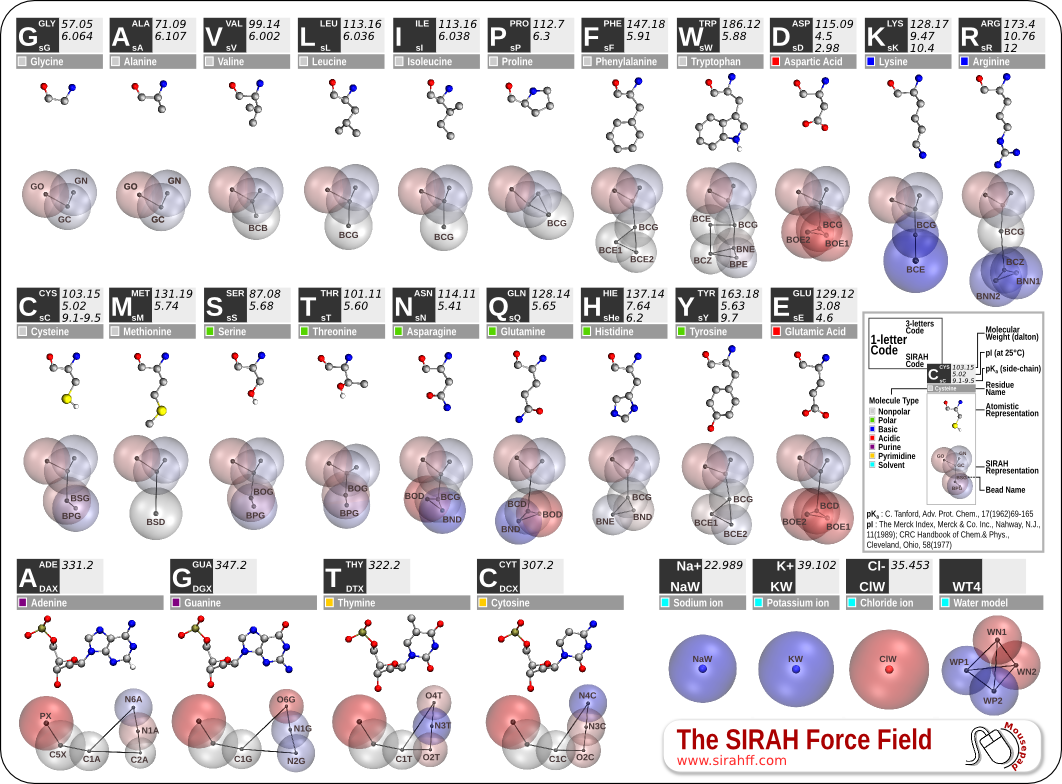
\includegraphics[width=0.8\linewidth]{2methods/pics/sirah_aa.png}
%
\caption[SIRAH force field amino acid and DNA description]{Description of amino acids and nucleic acids in the SIRAH force field. Reproduced from \cite{sirah_web}.}
\label{fig:sirah}
\end{figure}

The modelling of water in a coarse-grain force field is also critical: usually, a few water molecules are grouped together in one bead. This has two implications: water particles are large and thus cannot solvate very narrow pockets; moreover, collapsing the molecules in one single point in space removes the separation of charges and the characteristic dipole every water molecule should have is lost. The dipole of water is responsible for hydrogen bonds formation and for the electrostatic screening observed in an aqueous solution. Such screening can be roughly modelled tuning the relative dielectric constant, but as this is a mean field approach, it cannot account for local effects.
%
To partially obviate to that, SIRAH force field maps four waters to a tetrahedral molecule, with one bead on each vertex: all the bonds are rigid, and the structure serves the purpose of having a repartition of plus and minus charges, by assigning a positive charge to two vertices and the opposite charge to the other two, giving a polarisable structure. The geometrical arrangement reproduces the tetrahedral network of water molecules observed in its liquid state, which is characteristic of this fluid and tunes its remarkable properties.

Based on the above premises, SIRAH force field simulations of different peptides and proteins in solution proved to match the relative NMR results, showing a good reproduction of secondary structures; simulations of lipids randomly oriented in water showed the formation of an organised bilayer, and the expected behaviour of a few transmembrane proteins in model membranes was correctly reproduced \cite{Machado2018,Barrera2019}.

 
\subsection{The MARTINI force field}
The MARTINI force field is another popular coarse-grain description of biological molecules \cite{Marrink2007,Monticelli2008,DeJong2013}: developed originally with a focus on lipids, much earlier than SIRAH, it has been then extended to include proteins, small ligands and DNA/RNA molecules.

MARTINI opts for a four-to-one approach, i.e.\ four heavy atoms are grouped in one bead, resulting in a uniform graining and a coarser description than the SIRAH one. The only exception to this scheme is represented by rings molecules, where a two-to-one approach is needed to maintain the circular topology (consequently, these beads have a reduced mass with respect to the others, all described with the same mass value).

The number of bead types has been kept to the minimum necessary to represent biological molecules. They are organised systematically in polar, non-polar, apolar, or charged, and each type has a number of subtypes with increasing polarity to differentiate the chemical nature of the underlying atomistic structures.
%
This systematic parametrisation can be easily transferred to new compounds, without the need of introducing new bead types, analogously to what GROMOS does when parametrising small moieties.

Similarly to GROMOS, the MARTINI force field chooses a top-down approach to parametrise non-bonded interactions, tuning them against experimental partitioning free energies between polar and apolar phases, while bonded interactions are derived from reference all-atom information, in a bottom-up approach.
%
Specifically, they are designed so that the results from coarse-grain simulations match the structural data of the underlying atomistic geometry, derived either from available structures or atomistic simulations. For example the distribution of the length of a bond in a molecule would be mapped to its coarse-grain version (i.e. computing the corresponding bead-to-bead distance) and compared with the respective one obtained from coarse-grain simulations.

The four-to-one mapping implies that the amino acid backbone is represented by one bead only (Figure \ref{fig:martini_aa}), preventing the description of directional bonds which are key to reproduce the secondary structure. The bonded parameters partially account for this, favouring for each residue type the backbone conformation in which it is most likely found (as computed from the Protein Data Bank - PDB \cite{PDB}). When this is not sufficient, the protein can be constrained around a given structure through an elastic network model approach (ElNeDyn \cite{Periole2009}). However, both the backbone parametrisation and the use of ElNeDyn imply that conformational changes in the structure are penalised and therefore not well sampled in MARTINI simulations.
%
\begin{figure}[t!]
\centering
\subbottom[]{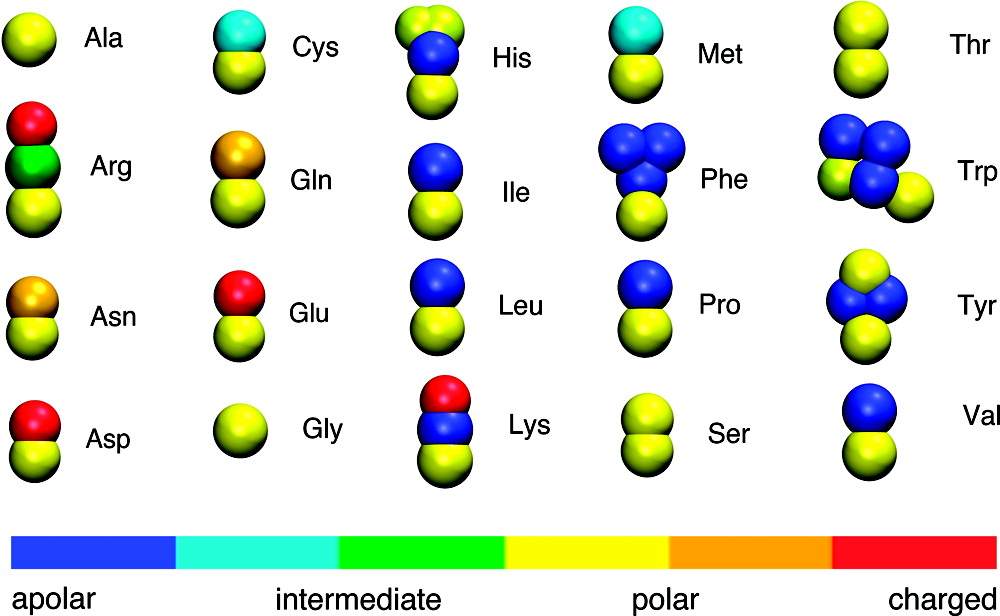
\includegraphics[width=0.7\linewidth]{2methods/pics/martini_aa.jpeg} \label{fig:martini_aa}} \\
\subbottom[]{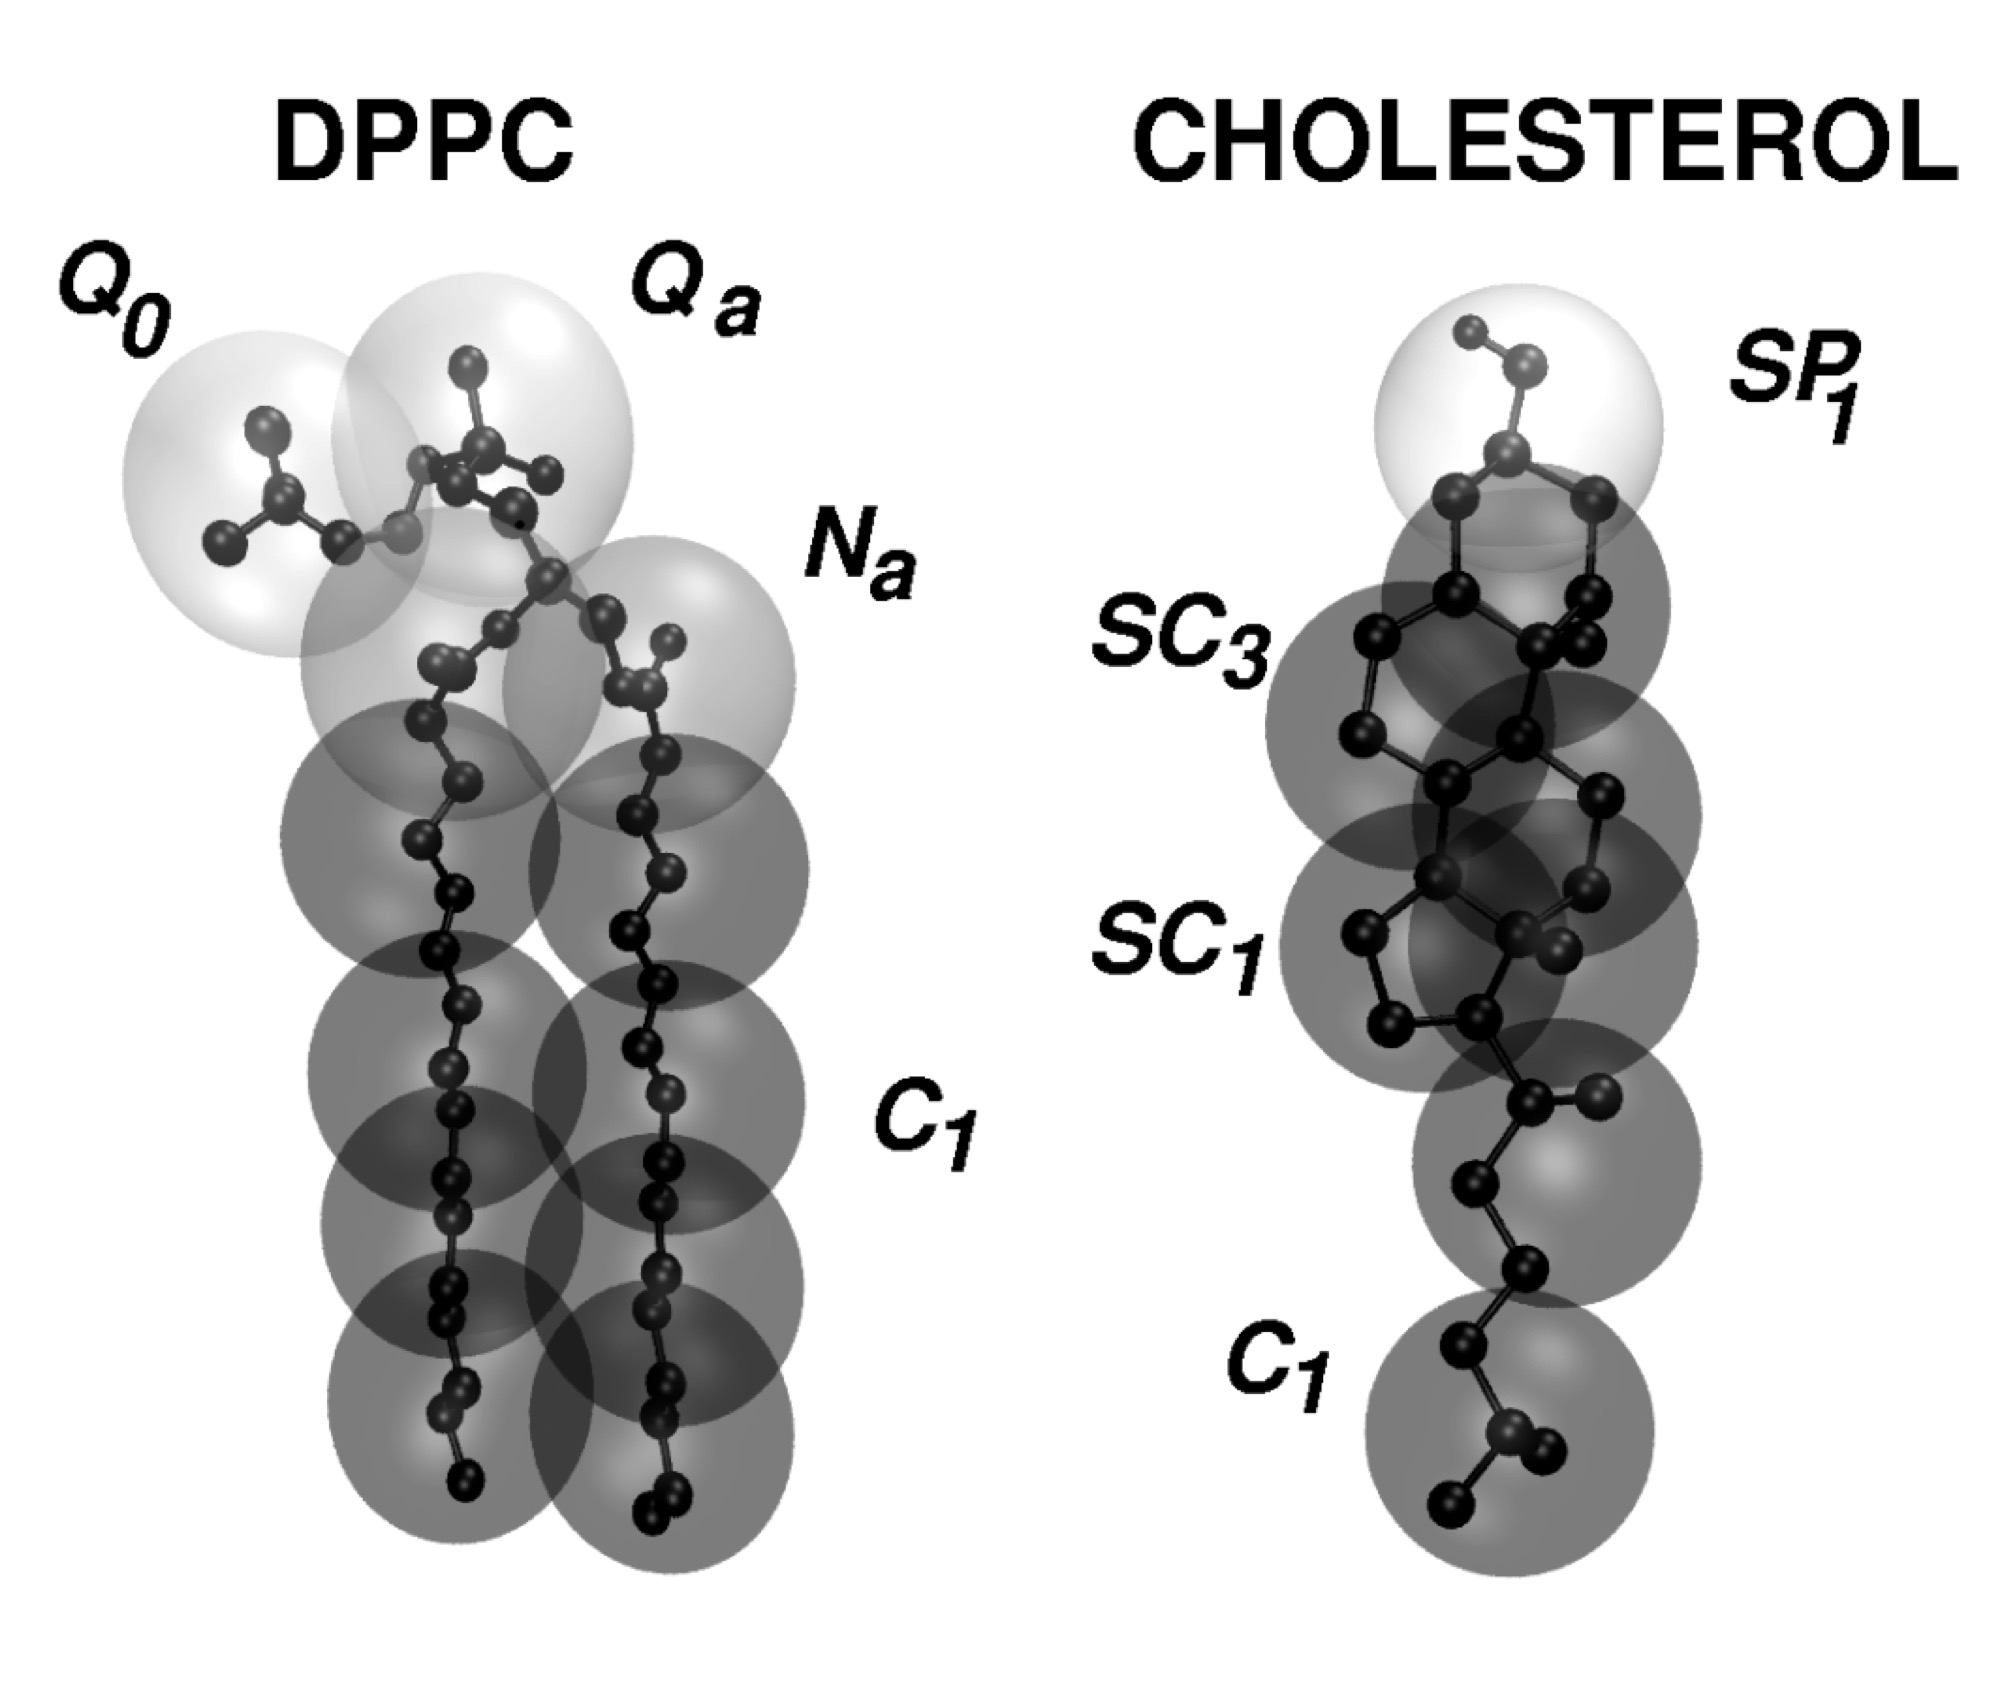
\includegraphics[width=0.4\linewidth, align=c]{2methods/pics/martini_lipids.jpg} \label{fig:martini_lip}}
\subbottom[]{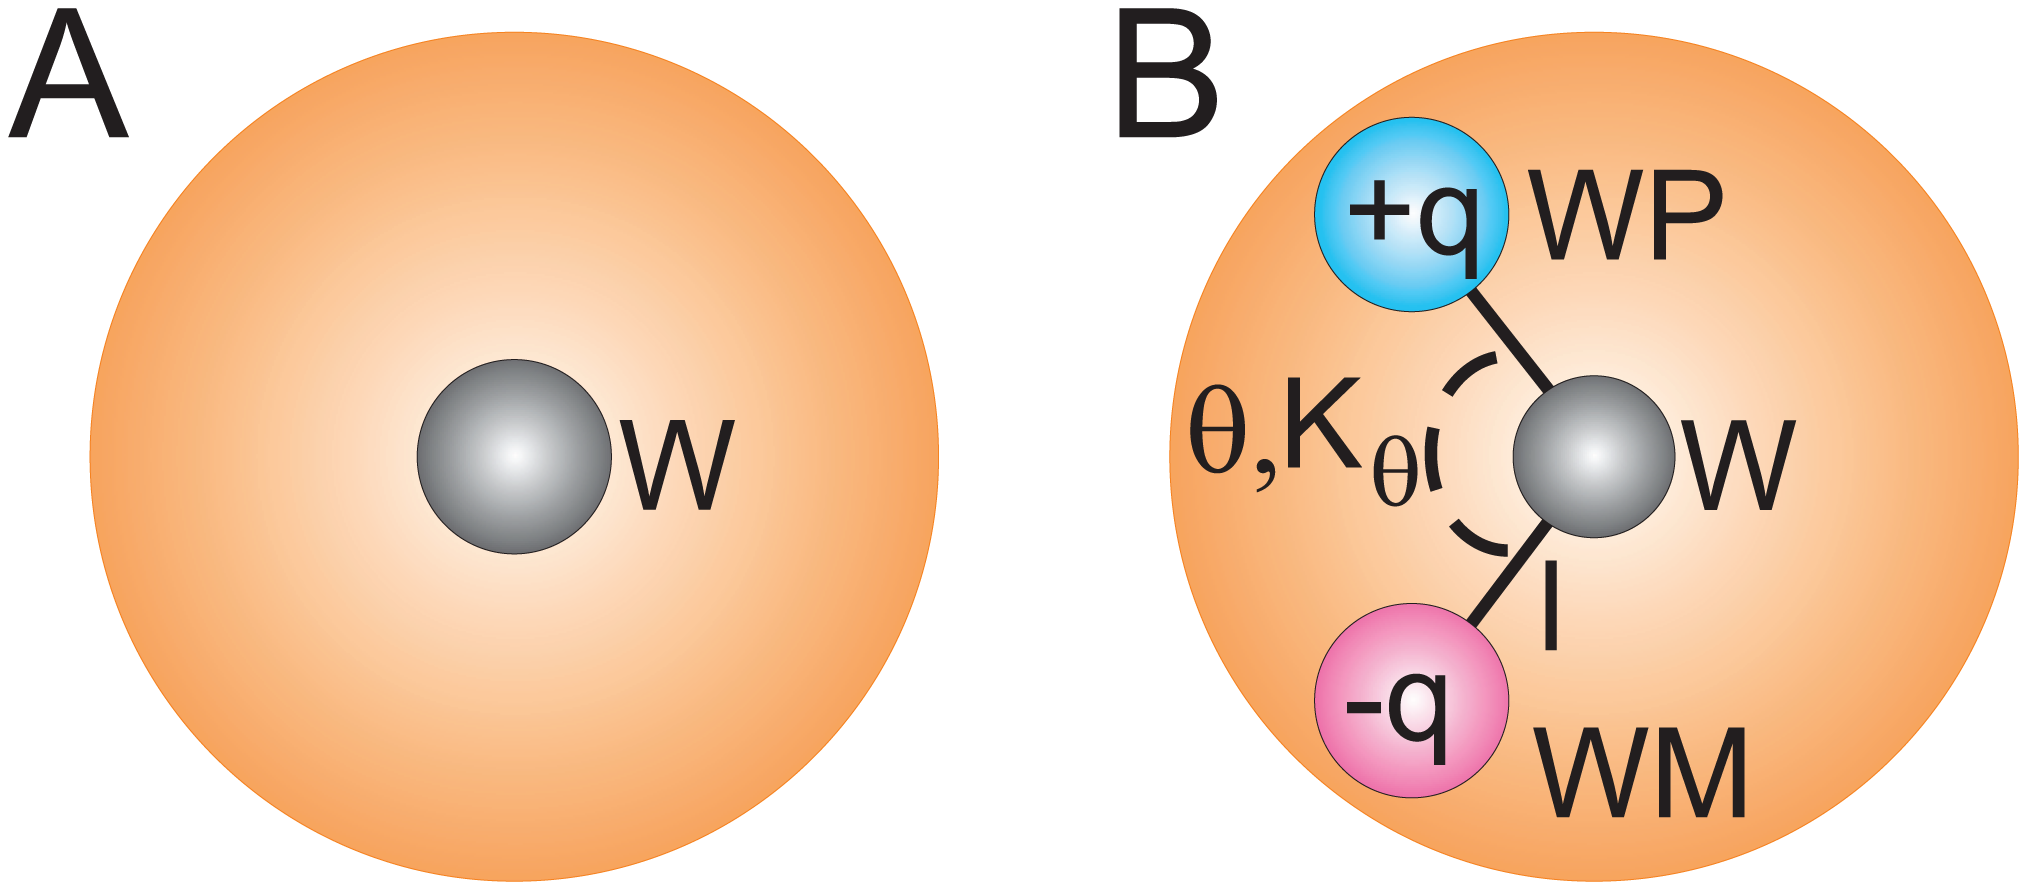
\includegraphics[width=0.35\linewidth, align=c]{2methods/pics/martini_polar.png} \label{fig:martini_w}}
%
\caption[MARTINI force field mapping for amino acids, lipids and water]{Description of amino acids (a), example lipids (b) and water models (c) in the MARTINI force field. In (c) the orange sphere represents the van der Waals radius of the central atom. Reproduced from \cite{Monticelli2008,calgary_site,Yesylevskyy2010}}
\label{fig:martini}
\end{figure}

The MARTINI force field provides two water models. The standard one groups four water molecules in one bead only (Figure \ref{fig:martini_w}, left), loosing the polarisability typical of water molecules, the effect of which is partially restored with the use of a high dielectric constant. The polarisable water model \cite{Yesylevskyy2010} maps instead four water molecule to a three-beads molecule (Figure \ref{fig:martini_w}, right) with a positive and negative charge on two of them, which can account for the water dipole. This model allows to revert the dielectric constant back to a value closer to 1.

Overall, the MARTINI force field pushes the limits of simplification to enhance the simulations speed-up, with considerable gain in efficiency with respect to atomistic or even SIRAH simulations. Despite it can not capture some fine details of the systems studied, it has been successfully applied to describe the behaviour of many biological membranes \cite{Khalid2019,Samsudin2017}, lipid self-assembly \cite{Marrink2007} and peptide-membrane binding \cite{Song2019}. The (re)introduction of a more detailed water model allowed the description of electroporation processes and the translocation of ions through bilayers \cite{Yesylevskyy2010}.

\subsection{Backmapping techniques} Coarse-grain descriptions are very effective in reproducing long time scales; however, to retrieve finer details after such extensive exploration, backmapping techniques have been designed to obtain atomistic configurations from the coarse-grain ones \cite{Wassenaar2015}. These backmapped structures can in turn be simulated at the atomistic level to explore the short time scale movements around such interesting conformation. The easy conversion between the two resolution, gave rise to many multiscale studies applied to biomolecular systems \cite{Lee2012}.


\section{Beyond the classical framework}

Without entering into the details, it is important to mention that the classical MD framework can benefit of additional terms aimed at improving its accuracy, and/or of specific techniques aimed at improving the
 sampling within accessible computer time.
 
\paragraph{Polarisability and quantum effects}
The first refinement possible is the introduction of polarisability, i.e.\ the displacement of electrons with respect to the nucleus, as a consequence of the surrounding electrostatic environment. None of the force fields mentioned above accounts for that, because electrons and nucleus of an atom are modelled as a unique object. Specific force fields have been modelled to include this effect, either on top of atomistic descriptions, as in AMOEBA \cite{Ren2003,Ponder2010}, Drude polarisable CHARMM \cite{Anisimov2004} or AMBERff02 \cite{Cieplak2001}, or in combinations with a coarse-grain descriptions, as in the ELBA force field \cite{Orsi2011}. Polarisability does improve the accuracy of simulations (see Chapter \ref{chapter:lip_par}, where it is discussed in the context of lipid tails parametrisation), but it can significantly slow down simulations.
%
Moreover, for biological processes governed by quantum mechanics - such as photosynthesis, DNA mutation processes or some enzymatic activities - many semi-classical hybrid techniques have been developed \cite{Ahmadi2018}. They combine computational quantum mechanical modelling methods, such as Density Functional Theory (DFT) or Hartree-Fock computations (HF) \cite{Shao2015}, with classical Molecular Dynamics to gain the accuracy of a quantum description in the region of interest and the speed up of a classical one in the surrounding areas.

\paragraph{Reduction of the number of degrees of freedom}
At the other end of the spectrum, tackling instead efficiency issues, many models have been implemented to reduce the number of degrees of freedom to deal with, among which the coarse-grain force fields already mentioned.
%
Another approach is constituted by the use of implicit solvent, where water is represented as a continuous medium, as opposed to explicit models which include all its particles \cite{Kleinjung2014}.
%
Models of implicit solvent can be based on different assumptions: for example the solute-solvent interactions can be taken as proportional to the solvent accessible surface area (SASA) of every particle of solute \cite{Fraternali1996,Kleinjung2003,Kleinjung2012,Fornili2012}, or instead can be derived from a solution of the Poisson-Boltzmann equation governing the charge density in a material, for example in the form of the Generalised Born equation \cite{Zhu2005} which is valid under particularly simple conditions.
%
Another technique to alleviate the computational burden is constituted by hybrid particle-field algorithms. The idea is to treat non-bonded interactions through a mean field approach, where atoms/beads move in the field generated by the others. The field does not need to be updated at every time step, as it is a collective and thus slowly evolving variable; moreover, for each particle only the interaction with the field, and not with all the neighbouring particles needs to be computed, reducing the computations effort further. This approach has been employed with a coarse-grain description of polymers and biological molecules in the OCCAM software \cite{Milano2009}.

\paragraph{Enhanced MD techniques}
Finally, computational strategies have been devised to bias the natural evolution of the system in order to enhance the sampling of many configurations, i.e.\ to speed up its pace.
%
This is particularly necessary when studying large-scale conformational transitions. This scenario corresponds to transitions between states separated by an energy barrier, but also matches cases in which we want to describe more accurately the phase space of a rugged landscape. Indeed very often, in the impossibility of understanding from first principles which states of a system are the most energetically favoured, and can therefore influence its macroscopic behaviour, MD simulations are run to explore the broadest possible set of them. The interpretation of such sampled states may become difficult and requires sophisticated analysis techniques.

To be noticed that, as biomolecular systems have a complex landscape dense of energy barriers, a realistic, limited time simulation usually samples regions around the initial configuration only.
%
In the simulations of proteins, this would often correspond to a structure derived from X-ray crystallography, which might not represent the native state of the protein in solution nor the functional form of interest.
%
An alternative could be the use of different pre-modelled initial structures so to reduce the sampling of states far from the equilibrium.

The challenges mentioned above have promoted the development of enhanced MD techniques. As a non comprehensive list, we mention replica-exchange algorithms \cite{Okamoto2004} which combine together multiple simulations held at different conditions, local potential-energy elevation (or metadynamics) \cite{Huber1994,Laio2002} which avoids the re-sampling of already visited conformations adding an energy penalty to them, umbrella sampling \cite{Torrie1977} which reconstructs free-energy barriers from simulations held at specific values of the coordinate along which the barrier exists, or finally simply the use of higher temperature to overcome energy barriers \cite{Kirkpatrick1983}.
%
To be noticed that a coarse-grain description of a system, by reducing the number of degrees of freedom, discards the high-frequency or less interesting ones, giving a smoother energy surface, so that the search is speed up both by the reduced computational load and by the fact that the system is not trapped into local minima due to the landscape roughness.


\section{MD and experiments: ensembles versus averages}
The validation of MD simulations is performed by comparison with experiments: the properties obtained experimentally are computed from the MD trajectory as well, and the latter compared with the former. If these are correctly reproduced, it is usually assumed that the simulation is sampling the correct ensemble of states. This holds if the properties of the simulation are not drifting away, namely the system has reached equilibration and it is thus in a stationary state.
%
Once the simulation has been validated, one can identify, from the conformations in the trajectory, the details of the processes responsible for the experimental outcome of interest, as such information is not accessible by the experiment itself.

The comparison however is not always easy, because of a fundamentally different focus that experiments and simulations have. The former measures often an average quantity in time and/or space, while simulations access the (hopefully complete) \emph{ensemble} of states that the system can visits and their occupancy, which in turn determines the macroscopic behaviour measured in the experiments.

In the case of a protein in solution, the \emph{ensemble} corresponds to the variety of shapes it adopts, which can differ significantly from the crystal-structures available. This flexibility is confirmed by small angle X-ray scattering (SAXS) and nuclear magnetic resonance (NMR) experiments, the results of which cannot be explained by a single-conformation scenario \cite{Bonomi2017,Kikhney2015,Kleckner2011}. In this context, only simulations can help in deconvoluting the results to map them back to the conformations and their relative contribution responsible for the outcome, uncovering their relative importance.

However, it is still challenging to compare experimental and simulations derived ensembles. Following from the example above, many different combinations of structures can match a SAXS profile, so in each specific case it is important to understand which are the relevant properties playing a role in the measured ensemble before attempting comparisons.

In general, in the validation of MD outcomes, it is necessary to have a critical attitude both in the case of agreement and disagreement with the experiment, and to interpret the result within the validity of the approximations performed by both of them \cite{VanGunsteren2008}.
%
Indeed, agreement may arise from either a simulation that reflects correctly the experimental system; but also when the property examined is insensitive to the details of the simulated trajectory, or it can be a result of compensation of errors, which is more likely to occur for systems with a high number of degrees of freedom (as biomolecular ones).
%
Similarly, disagreement may hint at an error in the simulation (either in the model, the implementation, or simply the estimated simulation's convergence) or an error in the interpretation and/or conditions of experimental set-up (either in the result itself or its interpretation), so that both must be carefully checked to improve a convergence in the agreement.
%
In this, some apparently negative results may suggest or stimulate new experimental settings to validate the hypotheses one was set to test \cite{Goncalves2013,Meissner2014}.

Moreover, simulations still suffer from the limited computational time accessible to effectively simulate the system in study: most of the times, the experimental system is simply too large to be reproduced and the time scale of the process too long to be accurately sampled. Simulations are thus confined to explore a restricted space, implying that the initial conditions must be chosen carefully to optimise the search and avoid any bias which might persist for the whole length of the simulation. The use of enhanced MD techniques does increase the chances of sampling relevant states, however it introduces a bias which must be removed or properly accounted for in the interpretation of the results \cite{Bernardi2015,Best2005,Barducci2010,Barducci2011,Mills2008}.
% Bernardi2015 general; Best2005 REX; Barducci2010,Barducci2011 metadynamics; Mills2008 umbrella sampling
Finally, one should keep in mind that the force fields used are far from optimal, partly because they rely on approximate functional forms, and partly because it is difficult to find experimental observables measured with the desired resolution able to discriminate between sets of parameters.

Despite the challenges outlined, Molecular Dynamics simulations have played a crucial role in disclosing important details behind biophysical processes and in unravelling molecular details not accessible to experiments. The following section will highlight a few of the many successes of MD simulations.


\section{MD simulations: successes} \label{sec:md_lit}
Consistently with the focus of this thesis, we will privilege examples of simulations investigating antimicrobial peptides as well as self-assembling ones, showing how computational techniques can help the design of novel molecules with improved specific characteristics.

\subsection{Simulations of antimicrobial peptides}
MD simulations of antimicrobial peptides are quite well documented since the first developments of the technique. Such peptides are a suitable system for a computational investigation as, in most of the cases, their mechanisms of action are not completely understood from the experimental information available (see Section \ref{AMP_mechs}). As experiments prove that even the mutation of one single residue in short AMPs can change remarkably the antimicrobial activity of the sequence (see Section \ref{sec:amp_design}), it is then clear that their action is governed by subtle atomic interactions, so that MD simulations, with their atomistic resolution, can help in understanding this aspect.

\paragraph{Systems} As mentioned in the previous chapter, it has been proposed that most AMPs act through a process of attraction to the bacterial membrane, possible aggregation with other copies of the same sequence, insertion, and membrane lysis. The time scales of the overall process are accessible if using coarse-grain techniques, but not - or rarely - atomistic ones.
%
For this level of description instead, the different steps are usually investigated separately, based on prior hypotheses: for example, the peptide can be positioned close to the membrane surface with an orientation known to promote binding (from experiments or based on energetic assumptions) \cite{Wang2012}, or again can be placed directly within the membrane core with different insertion depths, tilt angles and oligomerisation states to verify which configurations are the most disruptive ones \cite{Lipkin2017}. In this case, the full insertion process can only be reconstructed from a ``stepwise" knowledge combining the different states sampled and further exploring the intermediate regions if necessary.
%
For these reasons, the choice of the conformation to simulate, i.e.\ the initial conditions in terms of the mutual position of peptide and membrane, is crucial, as it likely biases the simulation towards the sampling of a particular subset of configurations, and this must be considered in the interpretation of the results. Recent advances are making possible the simulations of the full process even at the atomistic resolution for simple enough systems \cite{Ulmschneider2017,Sun2015}, as it will be shown in the following, nevertheless the ``stepwise" approach is still common and the preferred one in case of complex AMP systems.

\paragraph{Model membranes} The second important choice in the setup of a simulations of antimicrobial peptides concerns the model of the membrane to simulate. In an effort to keep complexity low, bacterial and mammal membranes can be modelled with a minimal number of lipids.
%
Very often, models of bacterial membrane retain as only key characteristic an overall negative charge, with about 25\% of the lipids being anionic ($-1\,e$ charge) and the rest being zwitterionic, i.e.\ neutral but with positively and negatively charged regions separate in space (see Chapter \ref{chapter:lip_par}) \cite{Lipkin2017,Wang2012,Zhao2018,Chen2019}.
For a model mammal membrane instead, only zwitterionic lipids are employed, with the occasional inclusion of cholesterol, as it is deemed important in describing more realistically their behaviour. \cite{Lipkin2017,Wang2012,Zhao2018,Chen2019,Risselada2008}.
Because of their simplicity, very similar or identical systems are used also in experiments \cite{Castelletto2016,Tang2009,Glukhov2005}, making possible a direct comparison with simulations.
Therefore, even if these simple membranes don't model accurately the structure of the cellular envelope, simulations and experiments of these systems can provide a first explanation of some steps of the antimicrobial activity, with the two techniques complementing and validating each other.

For example, an \emph{in silico} experiment simulated a dermicidin channel inserted into patches of phospholipids membranes with variable cholesterol content \cite{Song2019}. Nine membrane compositions were tested overall resulting in different membrane thickness, thus in a different orientation of the dermicidin channels inserted into it, with consequent variance in the conductance of the channel itself. This structure-function relationship shows the importance of an accurate membrane model to fully capture all the aspects of transmembrane protein activity as every change influences it. Notably, the simulations were performed with the coarse-grain model MARTINI, showing that a supra atomistic view retains enough details to investigate such systems.

Nevertheless, attempts to model more accurately cell membranes have been pursued. This can be performed at the atomistic level \cite{Piggot2011}
but the task is especially suited for a coarse-grain description, as the inclusion of all the elements of the cell membranes results in quite large systems for which atomistic computations started only in recent years to be affordable.
%
Accordingly, coarse-grain (MARTINI) simulations have been incorporating more and more components into model membranes, describing the bacterial inner membrane, the bacterial wall, and finally the combination of the two \cite{Khalid2019} (see Figure \ref{fig:ff}, bottom).
%
These large scale, coarse-grain simulations provide information on the mechanic characteristics of the system: for example, simulation of the outer membranes of Gram negative bacteria combined with the peptidoglycan layer (which, in bacteria, is positioned between the two membranes) elucidated how the distance between the two is variable, thanks to the presence of Braun's lipoproteins \cite{Asmar2018} which act as a bridge between them, and can bring them closer by bending and tilting.
%
On the other hand, the permeability of membranes to ions and small compounds needs to be assessed at the atomistic level, and to access informative simulation time scales, smaller and simpler systems must be chosen for the task (e.g.\ the inner membrane only), often together with enhanced MD techniques such as metadynamics, umbrella sampling, and replica exchange umbrella sampling. \cite{Sun2016,Piggot2011,Carpenter2016,Pokhrel2018}.

\paragraph{Force field comparison} Finally, simulations of the peptide interaction with a model membrane are clearly determined by the parametrisation of the force field employed for protein and lipids (and by their mutual consistency).
%
There are multiple evidence suggesting that different force fields produce very different outcomes when simulating the same system, under the same conditions. This is also valid for simulations of pure lipid patches (see Chapter \ref{chapter:lip_par}), resulting in incompatible values of area per lipid, organisation of the tails and energetic profiles across the membrane, and thus has an impact in the simulations of AMPs interacting with a membrane.

For example, Wang et al.\ \cite{Wang2014} run simulations of the antimicrobial peptide melittin with different force fields, namely CHARMM27 and 36 (for protein and lipids respectively) \cite{MacKerell1998,Klauda2010}, OPLS all atoms (for protein) and united atoms (for lipids) \cite{Jorgensen1996} and GROMOS 53a6 \cite{Oostenbrink2004} (and the TIP3P water model for all of them \cite{Jorgensen1983}).
%
Despite these parametrisation have similar values of partial charges on the different atoms, and similar bonded interactions at the protein level, the unfolding of melittin in the membrane was significantly different among them, with the CHARMM force fields suggesting an almost completely folded state for melittin bound to a membrane, in line with the NMR available results, while the other force fields promoted partial unfolding. Most likely this can be attributed to the fact that lipid and protein parametrisations are obtained separately and might present some inconsistencies. The most evident example is the OPLS case, for which an all atom description of lipids is not available and a mixed description has been adopted. In the case of GROMOS, both components are parametrised at the united atom level, but their mutual consistency might be questioned as well, as fully explained in Chapter \ref{chapter:lip_par}. In general, a united atom description is clearly less accurate than an all atom one, and in the case of lipids it has been postulated that it is not able to represent faithfully the dynamical processes happening in the hydrophobic tail region \cite{Chowdhary2013}.

A similar investigation has been proposed by Bennett et al. \cite{Bennett2016}, proving that the propensity of the synthetic AMP CM15 to form pores strongly depend on the force field used but also on some extent - at least at the time of the work - on the MD engine used (GROMACS compared to NAMD \cite{Phillips2005}). This should not come as a surprise because the membrane characteristics emerge from the collective behaviour of lipids, so that a small difference in the way their interactions are treated might be amplified resulting in different macroscopic outcome for the simulations \cite{Reisser2017}.

A more systematic study on the topic has been performed by Sandoval-Perez et al. \cite{Sandoval-Perez2017}, focussing on the reproduction of membrane-protein interactions in different force fields (GROMOS 54a7 \cite{Schmid2011}, CHARMM36, Amber14SB/Slipids \cite{Jambeck2012} and Amber14SB/Lipid14 \cite{Dickson2014}).
%
All of them were able to reproduce the overall positioning of transmembrane proteins in the case studies tested, together with their $\alpha$-helical and $\beta$-sheet content, while they showed discrepancies in the insertion angle for a short helical peptide (sybII) spanning the membrane.
%
The amino acid side chains insertion depth was also tested: the CHARMM force field suggested a deeper insertion for hydrophobic amino acids but the other parametrisations gave not so clear a distinction. In general, with the GROMOS force field, a higher energy is required to insert amino acids to the bilayer centre.
%
Interestingly, all parametrisations gave a very broad minimum for the insertion of Tryptophan, comprising the phosphate region of the phospholipid membrane tested, but also part of the tail and head regions. This is in line with the different interpretations given on the role of this amino acid for the action of antimicrobial peptides: either as an anchoring point positioned deeper in the hyrophobic region, or as a partner for hydrogen bonding with the hydrophilic heads.
%
The subtle differences between parametrisations lead to the conclusion that for every particular system tested, the comparison with at least one experimentally measured quantity would be the only way to assess the simulation performance accurately.

\paragraph{Simulations of membrane-peptide interaction: examples} Even in the context of a simplified model scenario and with the caveats coming from the chosen parametrisation, simulations of antibacterial peptides on a membrane have been successful in elucidating some of their mechanisms.
%
The first important contribution consists in the introduction of the disordered toroidal pore concept: as explained in the previous chapter (Section \ref{AMP_mechs}), the models of membrane poration due to AMPs consist often in ordered structures (see Figure \ref{fig:amp}) %
where many peptides gather together to contour a pore, and they are either in contact with the hydrophobic tails of the lipids (barrel-stave model), or with their head, as lipid molecules bend around the pore to keep their tails screened from the outside environment (toroidal pore model). However, simulations of the short helical peptide magainin MG-H2 \cite{Leontiadou2006}, among others, showed that a single copy of the helix, inserted at an angle with the normal to the membrane plane, was sufficient to displace the lipids around in a non organised manner and form a water-filled pore (Figure \ref{fig:dis_pore}).
%
\begin{figure}[t!]
\centering
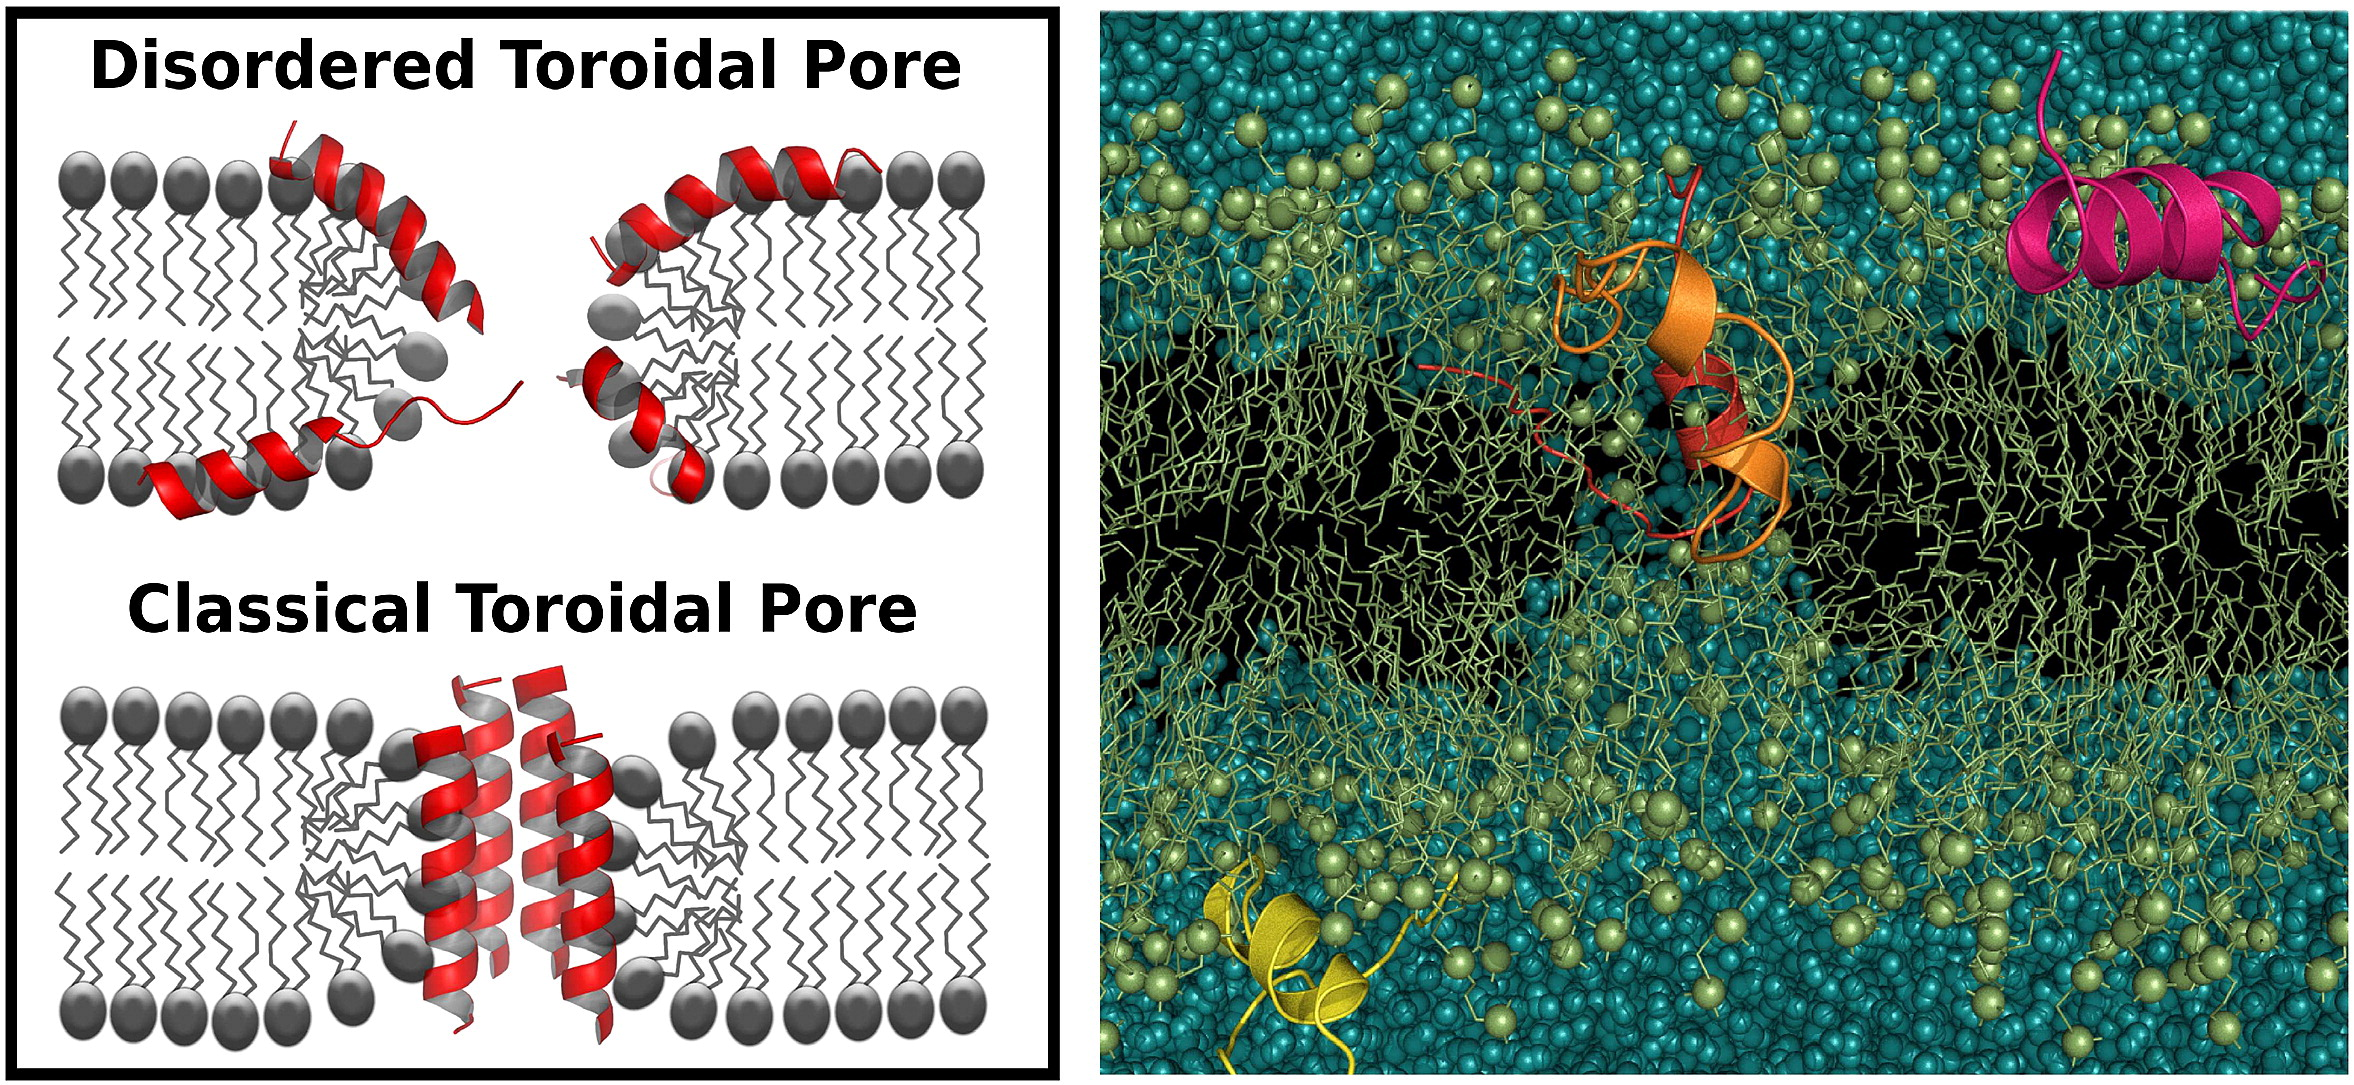
\includegraphics[width=0.8\linewidth]{2methods/pics/disordered_pore.jpg}
%
\caption[Disordered pore model]{(Left) A cartoon image comparing the disordered toroidal pore state (lack of a well defined peptide orientation) to the traditional view. (Right) A snapshot of the disordered toroidal pore from simulations of melittin in DPPC. Peptides in cartoon, lipids in lines, water and ions in bead representation. Reproduced from \cite{Sengupta2008}.}
\label{fig:dis_pore}
\end{figure}

% INITIAL CONDITION: SECONDARY STRUCTURE - KEPT/LOST
Regarding possible rearrangements of the antimicrobial peptide structure when interacting with a membrane, simulations of cathelicidin LL-37 on pure POPG (anionic) and POPC (zwitterionic) lipid patches showed that LL-37 has a propensity to bind to the former, as expected due to the opposite charge that membrane has with respect to the cationic peptide \cite{Zhao2018}. However the simulations highlighted also that, in contact with POPC, the helical secondary structure was lost, while the interaction with POPG preserved it, suggesting that the spatial arrangement of the residues, and not only the overall chemical character, is important for their action. Such type of information is hardly available to experiments or through a theoretical reasoning.

% INITIAL CONDITION: SECONDARY STRUCTURE - INFLUENCE ON BINDING
Further insights into the role of the secondary structure were obtained simulating the helical antimicrobial peptide CM15 nearby a POPC membrane, starting from a fully structured helix or from a coil configuration: Wang et al.\ \cite{Wang2012} proved that the interaction with the lipids is stronger when the peptide approaches the membrane in its disordered form rather than in a fully formed helix. This happens because of the larger flexibility of the coil arrangement which allows for more residues to come in contact with the membrane at once. Notable, the $\alpha$-helical fold binds as well to the membrane, but only after a time span larger than 100 ns, which would have been inaccessible up to a few yeas ago, potentially leading to wrong conclusions.

% INITIAL CONDITION - NO PRE-INSERTED PEPTIDE, SEE FULL TRANSLOCATION
The improvements in computational resources is slowly removing some of these obstacles, pushing the extent of simulation time to the microsecond timescale.
%
In a recent example, the translocation of the helical PGLa peptide through the membrane has been observed as a rare event, dependent on the concentration of the peptide, on the multi microsecond timescale without the formation of an organised pore \cite{Ulmschneider2017}. The \emph{in silico} experiment still benefited of an enhanced sampling in the form of a higher temperature used for the simulations, but no pre-insertion of the peptide was performed.  This study shed light on a possible mechanism of permeabilisation which is usually overlooked in favour of processes involving organised channels and pores. The fact that no organised neither disorganised pore is observed matches the experimental results which can not identify such structures for the peptide considered. 

% INITIAL CONDITION - NO PRE-INSERTED PEPTIDE, EXPLAIN POLYARGININES
Similarly, simulations were able to shed light on the mechanism of translocation of Arginine-rich peptides, proposing a mechanism of action on an otherwise puzzling problem \cite{Sun2015}. These sequences have high positive charge, but despite this, possess a high propensity to penetrate membranes, overcoming the hydrophobic region represented by the lipid tails. Very similar peptides where the Arginines were swapped with Lysins showed no significant penetration.
%
A commonly used explanation considers polyarginine translocation a quasi-equilibrium process, but this does not explain the selectivity against Lysins rich peptides.
%
After extensive simulations of the two systems (multiple, hundreds of nanosecond long runs, with two different force fields), the proposed mechanism involves the spontaneous formation of thermal pores: in some if these rare events, the transient pore would be occupied by a peptide (a precursor), which slows down its dynamics and thus closure. In such situation, the translocation of other copies of the peptide is highly favoured if their concentration is sufficiently high. Indeed, other copies of the peptide are driven to aggregate with the precursor inside the membrane and are then pushed toward the opposite side as there is a lower charge density in that region.
%
Differently from polyarginines, polylysins have a much lower aggregation propensity, so that the presence of a precursor peptide inside the membrane does not induce an enhanced insertion of further peptides.
%
\begin{figure}[t!]
\centering
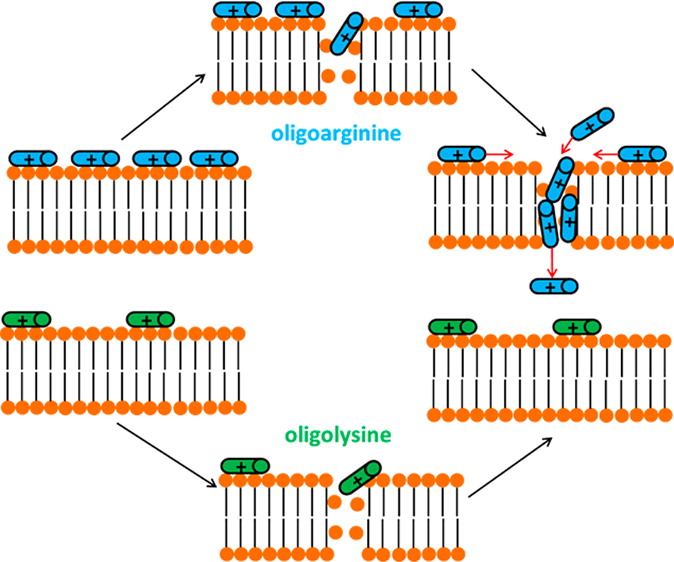
\includegraphics[width=0.6\linewidth]{2methods/pics/polyarg.jpeg}
%
\caption[Polyarginine translocation]{Cartoon representation of the different assembly mechanism that allow polyarginine but not polylysin to translocate through spontaneously formed pores. Reproduced from \cite{Sun2015}.}
\label{fig:polyArg}
\end{figure}

% OLIGOMERISATION
The last two examples mentioned bring the attention on whether and for which peptides oligomerisation is necessary for an efficient antimicrobial activity. MD simulations can offer insights on this aspect as well. Contrary to oligomerisation in solution, which can happen on shorter time scales, the spontaneous aggregation of peptides on a membrane surface requires a long time, as the structures must diffuse on the membrane to meet each other, and many other competing processes (such as insertion) are happening at the same time.

% OLIGOMERISATION - NO BIASED SAMPLING
A recent example of how MD elucidated oligomerisation mechanisms comes from simulations of maculatin (an helical AMP), which showed that the pores it forms can include a variable number of helices and thus assume many different conformations \cite{Wang2016}. The suggested process of pore formation proceeds via insertion of a single residue, closely followed by other ones which are able to penetrate the membrane thanks to the lipid defects already created by the first peptide.
% This is at odds with other models proposed beforehand, which include the insertion of already pre-formed peptide aggregates and suggest a unique ``rigid" form of the pore, but it is actually consistent with the experimental findings.

% OTHER NON AMP EXAMPLES
Similar investigations can be carried on also for other cell penetrating peptides, which are not antimicrobial: as such, some of them aim at inserting within cells without necessarily causing poration. One example is constituted by the influenza fusion peptides, which have been extensively studied with a simulation set up similar to the one mentioned for AMPs: a few copies of the peptide were positioned on a model membrane and their oligomerisation and insertion processes were followed in time, showing the formation of aggregates of different sizes which perturbed locally the membrane \cite{Haria2014,Collu2015}.

% OLIGOMERISATION - PRE-ASSEMBLED
To be noticed that, when investigating oligomerisation, the size of the system must necessarily be increased to include all the copies necessary to form the aggregates observed experimentally. As such, with the present accessible computer time, not all the systems can be investigated from unbiased initial conditions.
%
In the case of protegrin, a $\beta$-hairpin antimicrobial peptide which has been long though to act through the formation of transmembrane $\beta$-barrels, many variables can influence the outcome of the unknown final structure.
%
Even with the computer power available now, it is unlikely to sample all the possible conformations resulting in stable or transient $\beta$-barrel pores in simulations starting from a few peptides scattered on the surface, and this hinders the understanding of their relative importance.
%
To overcome such problems, a semi-systematic investigation has been carried on by Lipkin et al. \cite{Lipkin2017}, simulating different assembly (see Figure \ref{fig:ff}, top).
%
Microsecond long simulations discriminated which ones of these initial configuration formed stable pores for the whole length of the simulations, and the ones which were disrupted. As in the previous example, several different possibilities were found stable in solution, suggesting that single AMPs might have multiple mechanisms of insertion into membranes.

Most of the examples above employ atomistic descriptions of the system. Similar investigations have been carried on also using the MARTINI force field, indeed the coarse-grain description does capture the pore-forming behaviour of some AMPs.
%
As an example, simulations of maculatin and aurein on POPC membranes showed different propensities for pore formation versus aggregation, showing that the model retains enough details and chemical information to reproduce different membrane perturbing behaviours \cite{Balatti2017}.
%
Nevertheless, the developers of the MARTINI model themselves pointed out how some aspects of pore formation might not be captured in a satisfactory way \cite{Marrink2013}, for example the penetration of water can be misrepresented as can be intuitively expected from a model which clusters four water molecules together (indeed some pore conformations allow for the passage of fewer water molecule if not one at the time).

In general, the outlook of simulations of antimicrobial peptides interacting with membranes goes in the direction of reproducing longer time scales thanks to the enhanced computational power available, trying to match the experimental findings showing that many antimicrobial related processes happen at the microsecond scale or beyond.
%
This enhanced power would also reduce the need to use biased initial conditions or higher temperatures to speed up the simulations.
%
Moreover, gathering the contribution of the whole community, simulations will likely go in the direction of modelling more accurately the bacterial membrane, and while this is already at an advanced stage for coarse-grain simulations, it is still an ongoing process for atomistic ones.
%
Finally, the force field issue must be solved in collaboration with experimentalists, finding new tests and experimental quantities to compare the computational outcome with and make the different parameters sets converge toward a similar description of the phenomena observed, which is consistent with the experimental results.


\paragraph{Simulation-aided AMPs design}

The role of simulations in aiding AMPs design has been briefly sketched in Section \ref{sec:amp_design}. As pointed out, MD simulations are hardly a tool to analyse large dataset, therefore a systematic analysis can be performed for very small systems only, or, alternatively, the investigation can focus on a few selected sequences.

As already mentioned, when classifying AMPs, simulations can be helpful in integrating structural information which is otherwise lacking, when no crystal structure of the peptide is available. Such approach was followed by Liu et al. \cite{Liu2018} to complement the chemical information available on a dataset of short AMPs, and the overall information was used to feed a predictor of AM activity of novel sequences. Preliminary results showed that such structural information of minimal AM sequences improved significantly the ability of the predictor to discriminate whether a new sequence was suitable for antimicrobial activity or not.

Another commonly followed approach consists in using simulations to elucidate the reasons why a particular mutation is important and effective in terms of increased activity or decreased toxicity. Indeed, for short sequences, such mutation screenings can be afforded experimentally, thus there is little need to predict whether they would be beneficial. Rather, once assessed they are, it is interesting to understand why: for example, simulations of ovispirin and a mutant peptide with reduced toxicity showed that the bend in the helix in the latter was responsible for mitigating the interaction with mammal membranes and thus reducing haemolysis \cite{Khandelia2005}. Again, the mechanism of lipid disordering and insertion by indolicidin was assessed through MD, and the amino acids responsible for each of them separately were identified, so that mutants could be designed with either reduced toxicity or enhanced potency \cite{Tsai2009}. Finally, temporin and a derived sequence were investigate to discover that the mutant improved activity derived from a reduced aggregation propensity of the peptide in water, so that more copies were ready to bind to the membrane and thus disrupt it \cite{Farrotti2017}.

Many more examples can be listed, each with a slight different focus: the protocol of integrating simulations and design is usually customised according to the system in exam, as the field has not reached yet a systematic organisation.
%
However, it is clear that simulations used in conjunction with experimental testing can be used to optimise  already available AMP sequences, and thus contribute to device design rules for the creation of synthetic sequences with tailored properties.


\subsection{Simulations of self-assembling peptides}
Self-assembling peptides are another fascinating and challenging topic that MD simulations can help investigating. Simulating such systems implies different challenges with respect to the ones faced when simulating AMPs on membranes \cite{Frederix2018,Orsi2018}.

In theory, the set up of the system is quite straightforward: only the solvent characteristics and optionally the experimental salt concentration need to be matched, then a random initial configuration of the molecules - in the desired concentration - would allow the simulation of the process of interest.
%
In reality, reproducing the experimental conditions often implies working with very large systems: with the level of dilution of the solutions employed in the experiments, a considerable volume needs to be simulated to host enough copies of the peptide to observe the assembly of large enough oligomers.
%
However with this approach the time scale useful to witness a spontaneous assembly would greatly exceed the computational time available. For that reason, two main strategies have been adopted: coarse-grain simulations and the use of pre-assembled structures. Other routes include the choice of an implicit solvent model, or the use of other techniques such as Monte Carlo (a probabilistic exploration of the phase space rather than a dynamical algorithm) which can sometimes be less time consuming. Here, as we focus on MD simulations, we give a few examples of the first two strategies mentioned, which can be adopted in this framework.

Many studies have been performed with the coarse-grain MARTINI force field to witness assembly of surfactants \cite{Wu2012}, polymers \cite{Wang2012poly,Bochicchio2017} and lipids \cite{Lee2011,Brocos2012}, and a few focussed on peptides as well \cite{Guo2012,Seo2012}.
%
For example, the assembly in water of peptide amphiphiles (PAs) into cylindrical fibers has been simulated at the coarse-grain level \cite{Lee2012}, showing a transition from small micelles to longer fibres (Figure \ref{fig:PA}). This example of minimal PA structures is particularly interesting for the study of AMPs as well, as it shares with them the amphiphatic character, so that having a general knowledge on how similar sequences assemble together would help in tuning their aggregation properties in water prior to the delivery to the membrane.
%
In the work mentioned, pre-assembled fibres have been simulated as well at the atomistic level, to confirm their stability in solution.
%
\begin{figure}[t!]
\centering
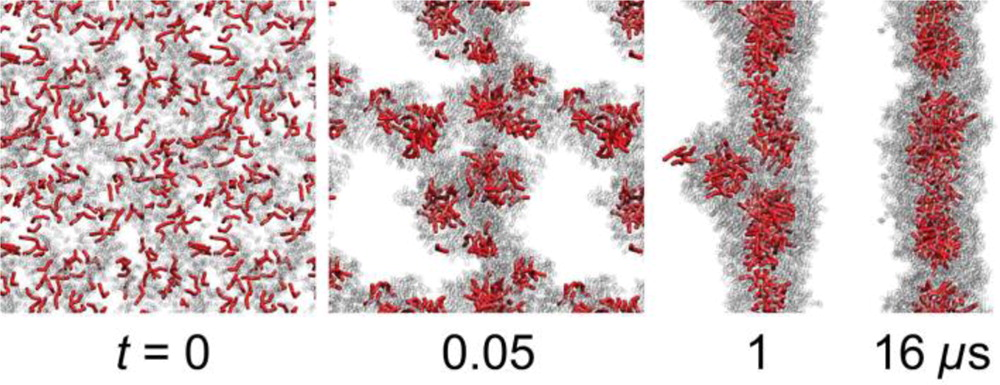
\includegraphics[width=0.8\linewidth]{2methods/pics/PA.jpeg}
%
\caption[Peptide amphiphiles assembly through MARTINI simulations]{Process of peptide amphiphiles (PA) fiber formation assessed through MARTINI simulations. Hydrophobic tails in red, peptides in gray \cite{Lee2012}.}
\label{fig:PA}
\end{figure}

The second approach consists in preparing the system in a pre assemble state that is somewhat suggested by experimental evidences and using MD simulations to verify whether the conformation is kept or it is disrupted, and which one out of many is the one most energetically favoured. It has been widely employed in cases where the final assembly was hypothesised to have a high degree of order, achievable only with a long sampling. 
%
This approach has been used to prove that a branched peptide can self-assemble in bilayers first, and then that a larger hypothetical structure assembled in the shape of a capsule was stable in the run time of the coarse-grain simulations employed. Specifically, the capsule has been build to match the peptide density on the self-assembled double layer and to respect the constraints derived from the presence of the curvature \cite{Gudlur2012}.

Similar approaches have been crucial in elucidating the assembly process of viral capsids: capsids are very large systems and the assembly of their protein subunits is mediated by energy barriers. For such reasons, already pre-assembled systems have been simulated to understand the interaction between the components and thus the first mechanisms of the assembly. This has been done recurring to ultra coarse-grain or elastic network models \cite{Grime2016} first, and only in the most recent advances to atomistic simulations \cite{Perilla2016,Hadden2018}. Additionally, smaller portions of a capsid can be simulated, to obtain a minimal information on the cohesion of its blocks \cite{AbiMansour2014}.


\paragraph{}
The examples above show how Molecular Dynamics simulations have been employed for the investigation of many different systems during the years, adapting the resolution, set up and the techniques related to better query the systems of interest. Such overview suggests then that simulations would be a suitable tool to investigate the system of interest of this work, namely the self-assembling antimicrobial peptide capzip. The two aspects of its behaviour will be studied separately, adopting the necessary approximations and strategies to make the simulations efficient and to query the related questions at each time.

\paragraph{}
The details of the systems simulated and the specific parameters used for each of the system simulated in the following chapters can be found in the relative sections, together with an extensive explanation of the motivation of the choices made.
\chapter{Lipid parametrisation} \label{chapter:lip_par}

\lettrine{S}{imulations} of lipids can be a challenging task, especially when the membrane simulated has not been tested experimentally, and thus no comparison can be performed on standard properties such as the area per lipid. Moreover, the parameters describing each lipid species must be carefully chosen, to aim at an accurate reproduction of the natural properties of the membrane.

The work performed in Chapter \ref{chapter:capzip_results} involved the simulation of a mixed membrane which, to our knowledge, has not been experimentally tested. Additionally, one of the lipids involved (DLPG) had not been parametrised before for the GROMOS force field.
%
The procedure of DLPG parametrisation brought to our attention the discrepancy existing between the GROMOS parametrisation of protein and the one employed for lipids, as the two of them are obtained through different procedures: fit to hydration properties for proteins, and quantum mechanics computations for lipids.

The set of lipid parameters derived originally from \citet{Chiu1995} and updated multiple times up to the work of \citet{PogerOrig}, is still regarded as a standard for phosphocholines, and thus used to validate the most recent parametrisation of the force field (GROMOS 54a8 \citep{Reif2012}). However, it does not take into account recent evolutions of the force field, aimed at reparametrising some constitutive moieties which happen to be also part of lipids.
%
For this reason, we performed a reparametrisation of the lipid head group which includes these new descriptions, aiming at an improved consistency with the rest of the force field and monitoring whether they would also improve the agreement with the experimental quantities.

The resulting parametrisation was successful in reproducing key properties such as the area per lipid, and proposed a different interaction with a test peptide with respect to the one outlines by the previous parameter set. Specifically, the new parameters promote a weaker protein-membrane interaction allowing simulations to be less biased from the initial conditions chosen. This is of crucial importance for all simulations in general, and in particular when the sampling is reduced due to computational resources issues.

This chapter consists of the paper ``Lipid Head Group Parameterization for GROMOS 54A8: A Consistent Approach with Protein Force Field Description", published in the \emph{Journal of Chemical Theory and Computation}, together with its Supporting Information. The project was conceived by Prof. Franca Fraternali, Dr. Christian Margreitter and myself. I carried out all the work, under their guidance; specifically I implemented the new parameter sets, performed and analysed the simulations and selected the best performing parameters to be released. References for the paper and its supplementary material are included separately after each of them (with a numeric notation). All references feature in the bibliography of this thesis as well.

<<<<<<< HEAD
%\includepdf[pages=1-19, nup=1x1, offset = 5mm 0mm, scale = 0.8, pagecommand = \pagestyle{thesis}]{4lip_par/proof.pdf}

%\includepdf[pages=1-6, nup=1x1, offset = 5mm 0mm, scale = 0.8, pagecommand = \pagestyle{thesis}]{4lip_par/Supplementary.pdf}
%\includepdf[pages=7-30, nup=1x2, offset = 5mm 0mm, scale = 0.8, pagecommand = \pagestyle{thesis}, landscape = true]{4lip_par/Supplementary.pdf}
%\includepdf[pages=31-33, nup=1x1, offset = 5mm 0mm, scale = 0.8, pagecommand = \pagestyle{thesis}]{4lip_par/Supplementary.pdf}
%\includepdf[pages=34-37, nup=1x2, offset = 5mm 0mm, scale = 0.8, pagecommand = \pagestyle{thesis}, landscape = true]{4lip_par/Supplementary.pdf}
%\includepdf[pages=38-43, nup=1x1, offset = 5mm 0mm, scale = 0.8, pagecommand = \pagestyle{thesis}]{4lip_par/Supplementary.pdf}
=======
\includepdf[pages=1-19, nup=1x1, offset = 5mm 0mm, scale = 0.8, pagecommand = \pagestyle{thesis}]{4lip_par/proof.pdf}

\includepdf[pages=1-6, nup=1x1, offset = 5mm 0mm, scale = 0.8, pagecommand = \pagestyle{thesis}]{4lip_par/Supplementary.pdf}
\includepdf[pages=7-30, nup=1x2, offset = 5mm 0mm, scale = 0.8, pagecommand = \pagestyle{thesis}, landscape = true]{4lip_par/Supplementary.pdf}
\includepdf[pages=31-33, nup=1x1, offset = 5mm 0mm, scale = 0.8, pagecommand = \pagestyle{thesis}]{4lip_par/Supplementary.pdf}
\includepdf[pages=34-37, nup=1x2, offset = 5mm 0mm, scale = 0.8, pagecommand = \pagestyle{thesis}, landscape = true]{4lip_par/Supplementary.pdf}
\includepdf[pages=38-43, nup=1x1, offset = 5mm 0mm, scale = 0.8, pagecommand = \pagestyle{thesis}]{4lip_par/Supplementary.pdf}
>>>>>>> 955964c0b525b9a3a6ada6e3e2ba179dc022b114


\section{Additional material: effects of membrane undulation}

During the revision process of the paper which constitute this Chapter, it was brought to our attention that membrane undulations might be incompatible with the computation of ApL performed from the sides of the simulation box. The more a membrane patch is deviating from a flat geometry, the more approximate would be such method.
%
Moreover, as the electron density profile is computed as an average over all the $x$ and $y$ positions, undulations of the membrane would result in a broader profile, with more uncertainty on the exact positions of the electron density peaks.

A brief comment on this appears on Section 2.5.1 of the paper, granting that the procedure chosen was suitable for the analysis of the simulations presented, and we would like to provide additional evidence to strengthen the case.
%
This analysis supports as well the choice of using the box sides approach in Chapter \ref{chapter:capzip_results} for simulation without or with low electric field, switching to a computation which takes into account undulations only for the highly curved membranes obtained with a high electric field.

The computation of ApL accounting for the membrane curvature is performed using a Fourier approach according to the work of \citet{Braun2011} and using the software made available from the same publication.
%
This allows to obtain the ratio between the ``true" area per lipid (i.e.\ computed taking into account the undulations of the membrane) and the projected one (i.e.\ from the box sides approach).
%
Figure \ref{fig:apl_und} reports the ratio ApL$_{\text{und}}$/ApL$_{\text{proj}}$ for each lipid and each parameter set: the values span between 1.0020 and 1.0046, which translates into an ApL correction between 0.20 and 0.46\%, or, in absolute value, 0.001-0.003 nm$^2$.
%
These discrepancies are lower than the standard deviation for any of the area per lipid computed, showing that the more accurate computation has no consequence for the purpose of evaluating the ApL and comparing parameter sets.
%
The parameter set showing less discrepancy is Chiu/54a7, compatible with the fact that on average it produces smaller area per lipid: a more packed bilayer results in less freedom for the lipids to undulate.

\begin{figure}[h!]
	\centering
	\includegraphics[width=0.5\textwidth]{4lip_par/pics/apl_localVSbox.pdf}
	\caption[Comparison between methods to compute ApL]{Ratio between area per lipid computed taking into account the undulations of the membrane (according to the procedure devised in \citet{Braun2011}) and the one computed from the projection on the plane parallel to the membrane. A value of 1 would be obtained for a perfectly flat membrane.}
	\label{fig:apl_und}
\end{figure}

Regarding the electron density, to check the influence of the averaging procedure over different locations of the patch, we computed the electron density for the phosphorus atoms on the full patch (256 lipid per leaflet), on a medium patch of roughly one forth in dimension (60 lipids per leaflet, see Figure \ref{fig:patch} for a scheme), and finally a small 12 lipids per leaflet patch. It must be noticed that the GROMACS software, while computing the density perpendicular to the bilayer plane (presently along the $z$ axis), centres the patch analysed around its center of mass, at each time step. This holds for GROMACS versions 5 onward, an version 2016.3 was used for all the analyses presented.

The resulting densities from the three different patches described above are normalised by the number of lipids present in each and compared. Figure \ref{fig:density_patch} shows that the profiles for the full and medium patches are almost identical, while the smaller patch produces narrower peaks.
%
Indeed, computing the full width at half maximum (FWHM) of these peaks, the FWHM of the small patch peaks is 16\% smaller than the FWHM of the large patch peaks.
%
However the distance between phosphorus peaks differ between patches by around 0.1 \AA\ only, showing that the undulations have an effect mainly (or only) on the peaks broadness.
%
As such, the hydrophobic thickness (measured as the distance between the phosphorous peaks) is virtually unvaried, and the difference imputable to the computing procedure is smaller than both the experimental thickness error and the differences arising from the use of different parameter sets.
%
Further analysis must be done on the Luzzati thickness estimate, which depends on the broadness of the water profile. However, it must be noticed that also for this measure, the range of experimental results is quite broad and thus, as for many properties assessed in the paper, likely to be larger than the differences which can derive from the analysis procedure.

\begin{figure}[t!]
\centering
\subbottom[]{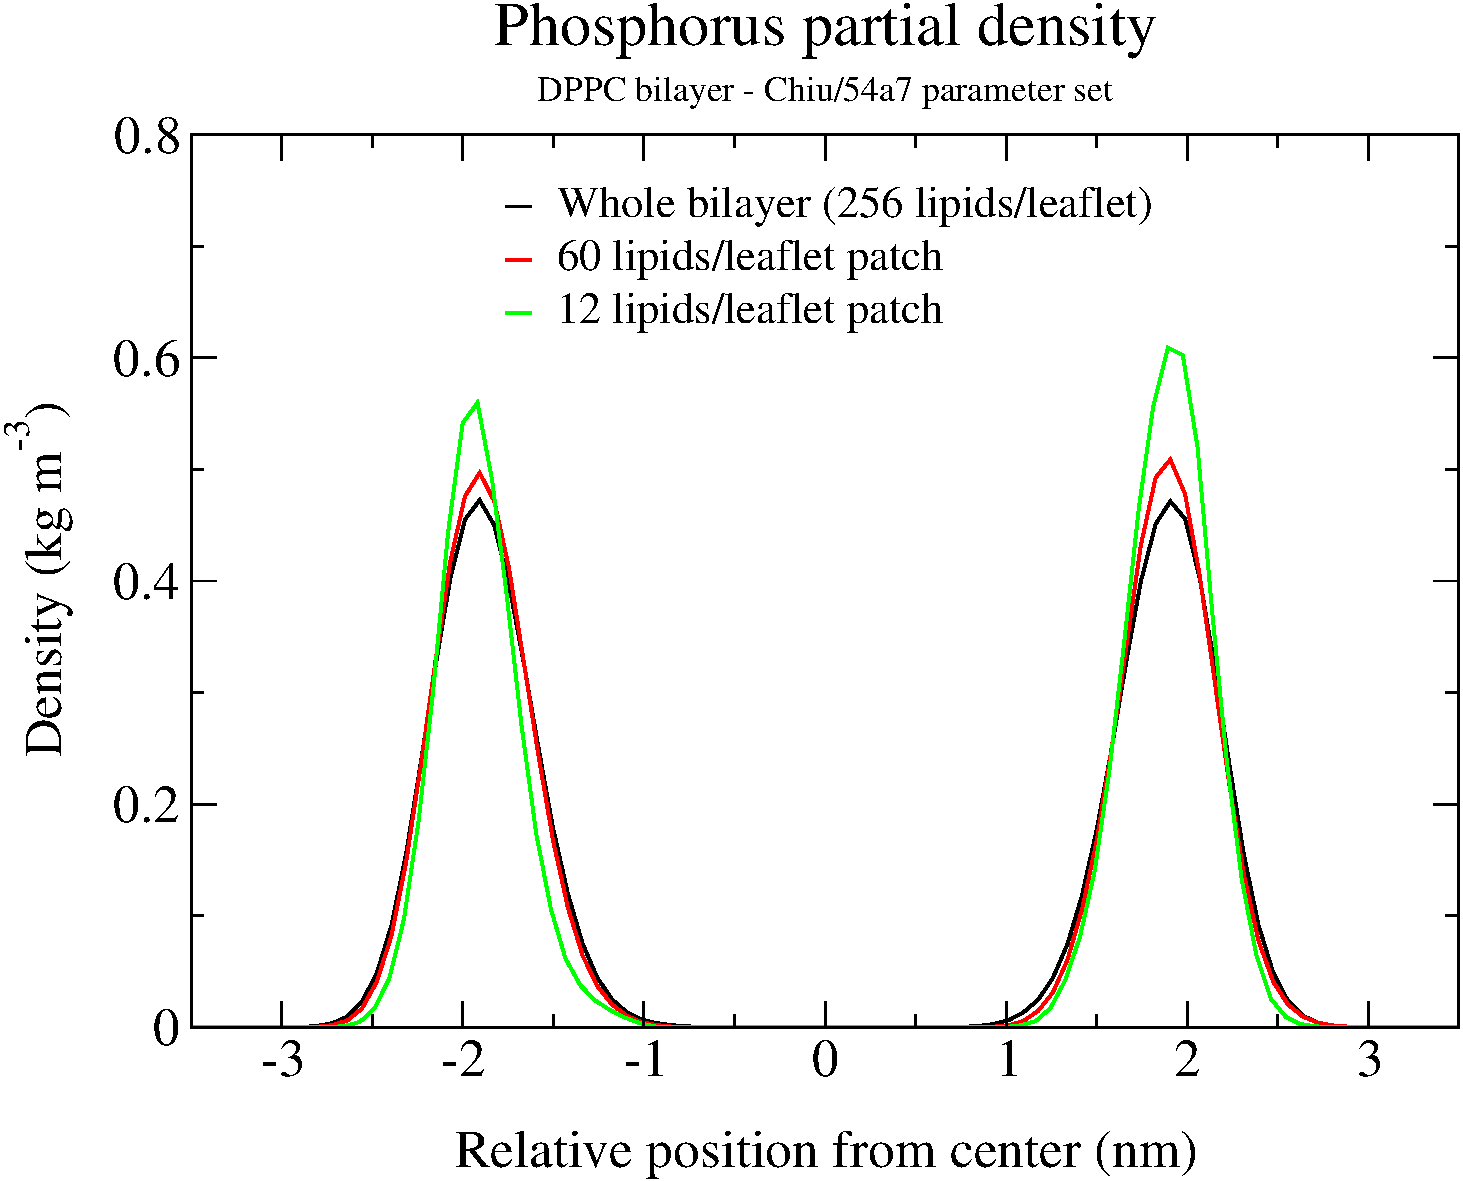
\includegraphics[width=0.55\linewidth, align=c]{4lip_par/pics/compare_density} \label{fig:density_patch}}
\subbottom[]{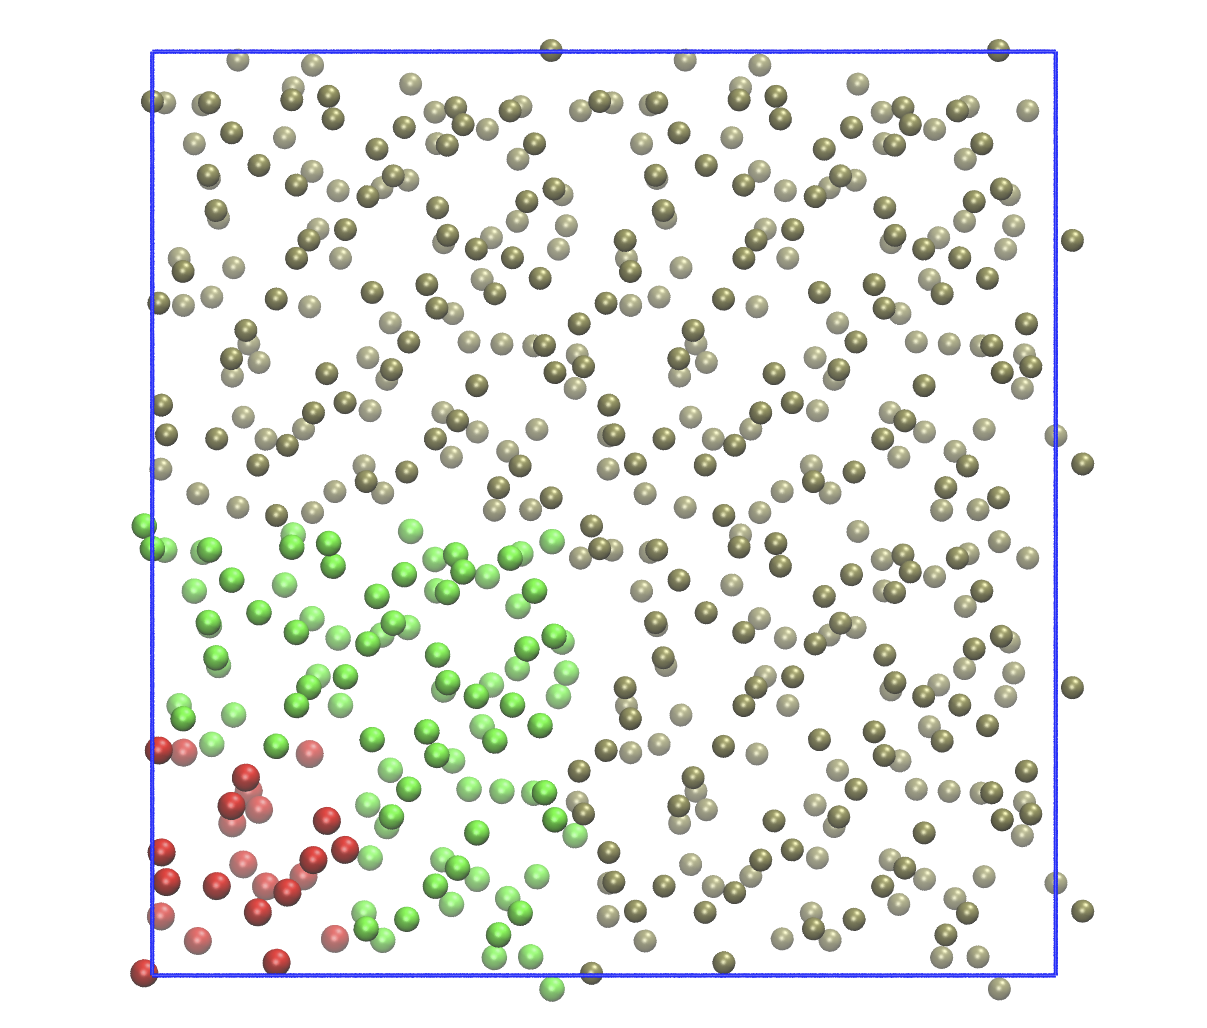
\includegraphics[width=0.35\linewidth, align=c]{4lip_par/pics/patches.png} \label{fig:patch}}
%
\caption[Control computation on bilayer electron density calculation]{(a) Electron density of the phosphorus atom computed on the full membrane, a medium and a small patch. (b) van der Waals representation of the phosphorus atoms of the DPPC lipid bilayer (initial configuration) used for simulations. The simulation box is highlighted in blue. The green plus red regions constitute the medium patch mentioned in the analysis; the red one constitute the small patch.}
\label{fig:density_check}
\end{figure}

\nocite{Abraham2015,Aurenhammer1991,Berendsen1984,Berendsen1995,Berglund2015,Borle1983, Borle1985,Botan2015,Bransden2003,Braun2011,BULDT1978,Castelletto2016,CelineAnezo2003, Chan2006,Chan2007,Chandrasekhar2003,Chandrasekhar2004,Chandrasekhar_vanGunst2001, Chandrasekhar_vanGunst2002,Chiu1995,Chiu2009,Chowdhary2013,Clarke2001,Cocucci2017, Cooper2000,Davis1981,deVries2004,Dickson2014,Ding2015,Doktorova2017,Douliez1995, Douliez1998,doux2012,Einstein1956,Entova2018,Essmann1995,gromacs_man,gromos43a1, Gurtovenko2007flip,Gurtovenko2009,HariLeontiadou2006,Hart2012,Hess1997,Hodder2001, Huang1982,Huang2017,Hwang1998,Jean-Louis2006,Jia2011,Johner2016,Kandasamy2004,
Khalid2015,Klauda2010,Kucerka2011,Kucerka2015,Kukol2009,Lairion2002,Leontiadou2004,
Leontiadou2007,Lewis1987,Lindblom2009,Lipkin2017,Lopes2017,Ma2017,Mabrey1976,Maier2015,
Malkia2004,Margreitter2017,Marinov1996,Marrink2001aggr,Marrink2003,Marrink2005,
McIntosh1986,Miyamoto1992,Mulliken1955,Nagle2000,Nagle2017,Nagle2019,Nguyen2005,
Oostenbrink2004,openStruct,Pan2012,Petrache2000,Petrov2013,Pickar1978,Piggot2011,
Piggot2012,Piggot2017,Pino-Angeles2016,Pluhackova2016,Poger2016,PogerOrig,PogerValid,
Rand1988,Reif2012,Reif2013,Reisser2017,Risselada2008,Schamberger2002,Schibli1999,
Schmid2011,Scott2017,Semchyschyn2004,Sengupta2008,Sharpe2010,Shi2003,Skjevik2015,
Sohlenkamp2016,Starke-Peterkovic2009,Strom2002,Sun1994,Tieleman1998,Tieleman2006flip,
Tironi1995,Ulrich1990,Ulrich1994,Uppulury2015,VanLehn2014a,VanLehn2014b,Venable2017,
Vermeer2007,Vernier2006,Vivcharuk2008,Vogele2018,Wang1994,Wang2006,Wang2012,
Warshaviak2011,Zhang2001,Zhao2000}


\appendix
\renewcommand{\appendixname}{}

\setcounter{chapter}{-1}
\chapter{Appendices} \label{appendix}
\renewcommand{\thechapter}{A}

%%%%%%%%%%%%%%%%%%%%%%%%%%%%%%%%%%%%%%%%%%%%%%%%%%%%
%%%%%%%%%%%%%%%%%%%%%%%%%%%%%%%%%%%%%%%%%%%%%%%%%%%%

\section{Supplementary material}
\label{sec:SI}
Supplementary material can be found at \url{https://github.com/imarzuoli/????} and includes Supplementary videos of:
\begin{itemize}
\item atomistic simulation of the buckyball bilayer - 100 ns (\url{SI_M1_GROMOS_buckyball.mp4});
\item SIRAH and Polar MARTINI simulations of the buckyball bilayer and monolayer - 1 $\mu$s (\url{SI_M2_SIRAH_buckyball_BIandMONO.mp4} and *\url{SI_M3_PolarMARTINI_buckyball_BIandMONO.mp4});
\item atomistic simulation of poration of a model bacterial model membrane under the combined action of the pentagonal capzip subunit and an external electric field of 130 mV/nm - 60 ns (\url{SI_M4_GROMOS_capzip_bacterial_E130.mp4});
\item standard MARTINI simulation of a buckyball bilayer approaching a bacterial and mammalian model membrane - 10 $\mu$s (\url{SI_M5_stdMARTINI_capzip_bacterial.mp4} and \url{SI_M6_stdMARTINI_capzip_mammalian.mp4});
\item Polar MARTINI simulation of a buckyball bilayer porating a model bacterial membrane under the effect of a 40 mV/nm external electric field - 200 ns (*\url{SI_M7_PolarMARTINI_capzip_bacterial_E40_poration.mp4}).
\end{itemize}


\section{Software developed}
\label{sec:Appendix_software}

The simulations and analysis of capzip systems prompted the development of tools to facilitate the set up of simulations, or their analysis.
%
The scripts and packages developed, to be used in conjunction with the standard analysis tools provided by the GROMACS and MDAnalysis softwares, can be found at \url{https://github.com/imarzuoli/MDtools} and include:
\begin{itemize}
\item python functions to perform the analysis of contacts as in Section \ref{sec:results_cap} (\url{contacts_analysis.py}); functions to perform the hydration analysis as in Section 3.4 of Chapter \ref{chapter:lip_par} (\url{an_min_hist.py});
%\emph{delete_water.py}: a script to delete water molecules in a given slice of space (perpendicular to either x, y or z)

\item a python module to manipulate multi-branched peptide topology files in the GROMACS format for GROMOS simulations (\url{MD_mutate_and_manipulate.py}).

\end{itemize}


\backmatter
\bibliographystyle{naturemag}
\bibliography{thesis_ref}
%\bibliographystyle{plain}


\end{document}
